\documentclass[12pt, a4paper]{article}
\usepackage{scrextend}
\usepackage{titlesec}
\usepackage{graphicx}
\usepackage{amsmath}
\usepackage{amssymb}
\usepackage{amsfonts} % for the real number symbol
\usepackage{geometry}
\usepackage[unicode]{hyperref}
\usepackage{titlesec}
\usepackage{titletoc}
\usepackage[sorting=nyt]{biblatex}
\usepackage{xurl}
\usepackage{enumitem}
\usepackage{indentfirst}
\usepackage{multirow}
\usepackage{tocloft}
\numberwithin{equation}{section} % number equations by section
\renewcommand{\figurename}{Att.}
\renewcommand{\contentsname}{Saturs}
\renewcommand{\labelenumi}{\arabic{enumi})} % lists with 1)
\renewcommand{\cftsecfont}{\scshape\large}
\renewcommand{\cftsecaftersnum}{.}
\renewcommand{\cftsecleader}{\cftdotfill{\cftdotsep}}
\renewcommand{\cftsecpagefont}{\normalfont}
\setlist{nosep}
\parindent=1cm
\linespread{1.213} % equivalent to 1.5 in word, experimentally.
\addbibresource{refs.bib}

\geometry{
    a4paper,
    lmargin=30mm,
    rmargin=20mm,
    tmargin=20mm,
    bmargin=20mm
}




\titleformat{\section}
    {\centering\normalfont\large\bfseries}{\thesection . }{0.2em}{\MakeUppercase}
\titleformat{\subsection}
    {\centering\normalfont\large\bfseries}{\thesubsection . }{0.2em}{}
\titleformat{\subsubsection}
    {\normalfont\normalsize\bfseries\itshape}{\thesubsubsection . }{0.2em}{}
\titlespacing*{\subsubsection}{0pt}{6pt}{0pt}

\begin{document}
\begin{titlepage}
    \begin{center}
        \vspace*{3cm}
        
        LATVIJAS UNIVERSITĀTE

        DATORIKAS FAKULTĀTE

        \vspace*{4cm}

        \large\textbf{ATDARINOŠĀS MAŠĪNMĀCĪŠANĀS PIELIETOJUMS ROBOTIKĀ}
        
        \vspace{2cm}
        \normalsize{MAĢISTRA KURSA DARBS}
         
             
    \end{center}
    \vspace{3cm}
    \begin{addmargin}[18em]{0em}
    Autors: \textbf{Pēteris Račinskis}
    \end{addmargin}

    \begin{addmargin}[18em]{0em}
    \hspace{1cm} Stud. apl. Nr. pr20015
    \end{addmargin}

    \begin{addmargin}[18em]{0em}
    Darba vadītājs: Dr. sc. comp. Modris Greitāns
    \end{addmargin}
         
    \vfill
    \begin{center}
    RĪGA 2022
    \end{center}
 \end{titlepage}
\newpage

\section*{Anotācija}
\thispagestyle{empty}

\newpage
\phantomsection
\section*{Abstract}
\thispagestyle{empty}


\newpage
\phantomsection
\section*{Autoreferāts}
\thispagestyle{empty}
\newpage

\newpage

\addtocontents{toc}{\protect\thispagestyle{empty}}
\tableofcontents
\thispagestyle{empty}
\newpage
\setcounter{page}{7}

\phantomsection
\section*{Ievads} % * nepieliks numuru pie nosaukuma
\addcontentsline{toc}{section}{Ievads}


Mašīnmācīšanās šobrīd tiek plaši uzskatīta par vienu no aktuālākajām datorzinātņu pētniecības nozarēm \cite{no_shit}. Pēdējās desmitgades laikā šī pētniecības lauciņa popularitāte ir daudzkārt pieaugusi, pateicoties galvenokārt diviem faktoriem: ļoti vispārīgiem neironu tīklu modeļiem un skaitļošanas resursu veiktspējai, kas beidzot ļāvusi šos, teorētiski jau pagājušajā gadsimtā \cite{mcculloch1943logical, linnainmaa1970representation, fukushima1988neocognitron} iedomātos, mākslīgā intelekta uzbūves elementus realizēt praksē. Starp uzdevumiem, kurus izdevies realizēt, aizstājot mēģinājumus rast analītiskus risinājumus ar pietiekami jaudīgiem neironu tīklu modeļiem, ir semantiskas nozīmes meklēšana attēlos \cite{krizhevsky2012imagenet}, tekstu korpusu analīze un ģenerēšana ar "izpratni" par to saturu \cite{vaswani2017attention} un visspējīgāko spēlētāju pārspēšana nepilnīgas informācijas spēlēs ar neap-tverami milzīgiem iespējamo stāvokļu permutāciju skaitiem \cite{silver2016mastering}.

Nav arī īpaši grūti atrast vēsturisko saikni starp mākslīgo intelektu un robotiku. Tautas iztēlē termins ``robots'' drīzāk droši vien iezīmēs zinātniskās fantastikas radītos personāžus -- mehāniskas būtnes, kas spēj patstāvīgi darboties neierobežotā vidē un risināt sarežģītus uzdevumus -- nevis pieticīgākus, reāli pastāvošus un ražotnēs rodamus industriālos robotus. Šī pati zinātniskā fantastika radījusi arī nesaraujamu saiti starp robotiem un mākslīgo intelektu \cite{asimov2004robot}. Neformālas diskusijas par mākslīgo intelektu bieži vien plūstoši pāriet diskusijās par ar šādu intelektu aprīkotiem robotiem, un, neizbēgami, dažnedažādiem šo intelektuālo sistēmu radītiem draudiem mūsu sabiedrībai. Protams, zinātne ne vienmēr seko populārzinātniskās iedomas lidojumam, taču šāda saikne ir visnotaļ pamatota -- spēja mācīties no paraugiem vai patstāvīgi, pielāgoties savai apkārtnei ir ārkārtīgi noderīga. Daudzi uzdevumi, kuru risināšanai varētu pielietot robotus, ir sarežģīti nevis to fizikālajā izpildē, bet tieši vadības uzdevuma formulēšanā un realizācijā -- lai to ilustrētu pietiek vien aplūkot kādu nejauši izvēlētu sarakstu ar robotikā aktuālām problēmām \cite{popsci}.

Atdarinošā mašīnmācīšanās (\textit{imitation learning}) ir viens no paņēmieniem, ar kuriem tiek mēģināts risināt šādas sarežģītas vadības problēmas. Lai gan pamatu pamatos nevar apgalvot, ka tā ir tikai robotikai piemērota metožu saime, lielākā daļa izpētes virzīta tieši šajā virzienā \cite{attia2018global}. Problēmas tiek formulētas kā fizikālu (vai nosacīti fizikālu -- virtuālās vidēs simulētu) procesu kontroles uzdevumi, un risinājumi tiek rasti no pēc iespējas mazāka skaita veiksmīgas darbības piemēru \cite{attia2018global}. Mašīnmācīšanās nozarē bioloģiskas analo-ģijas un iedvesma nav nekāds retums, un savā ziņā šāda mācīšanās  atspoguļo vienu no izplatītiem paņēmieniem, kā cilvēki vai sabiedriski dzīvnieki nodod prasmes viens otram - demonstrējot. Nevar nepieminēt, ka izpēte šajā jomā bieži aizņemas pieejas un iespaidojas no rezultātiem, kas gūti ar stimulēto mašīnmācīšanos (\textit{reinforcement learning}) - savā ziņā vispārīgu, pašmācībai un treniņam analoģisku paņēmienu. Arī abu metožu apvienojums ir ideja, kas pavīd visai regulāri -- cerībā, ka, atdarinot ekspertus, var ātrāk nonākt pie derīgām stratēģijām, kas var kalpot kā sākumpunkts dziļākai pašmācībai \cite{hester2018deep}. Visbeidzot, pavisam nesen sasniegti ļoti pārliecinoši rezultāti ar teksta un cita veida virkņu regresijai paredzētiem modeļiem arī atdarināšanas jomā \cite{reed2022generalist}. Tas liecina, ka varbūt tieši laikrindu modeļi ir atslēga veiksmīgai apmācībai ar paraugdemonstrācijām.

\phantomsection
\subsection*{Darba mērķis un struktūra} % * nepieliks numuru pie nosaukuma
\addcontentsline{toc}{subsection}{Darba mērķis un struktūra}

Maģistra darba tēma izvēlēta ar Elektronikas un datorzinātņu institūta personāla palīdzību, meklējot šobrīd aktuālu pētniecības virzienu. Izvērtējot dažādus pieejamos variantus, izvēlēts pētniecības virziens -- atdarinošā mašīnmācīšanās -- un konkrēts motivējošais uzdevums -- atkritumu šķirošanas līnijas robots, kas izmanto mešanas kustības. Darba izstrāde attiecīgi notikusi institūta Robotikas un mašīnuztveres laboratorijā. Tur paralēli noris cita, radniecīga pētnieciska darbība -- gan atkritumu šķirošanas procesu automatizācijā, gan stimulētās mācīšanās metodēs. 

Šī darba mērķis ir noskaidrot, vai atdarinošās mašīnmācīšanās metodes ir piemērotas motivējošās problēmas risināšanai, izvērtēt dažādu paņēmienu un aktuālāko rezultātu izmantošanas iespējas un izstrādāt prototipu procesam, kura gaitā tiek iegūtas demonstrācijas un apmācīti modeļi, kas izpilda doto uzdevumu. Attiecīgi, maģistra darba pamatdaļa sastāv no četrām nodaļām:
\begin{enumerate}
    \item vispārīga nepieciešamo teorētisko pamatu izklāsta, kur īsi apskatīti parametrisku modeļu, lēmuma procesu, robotikas matemātiskie formālismi;
    \item atdarinošās mašīnmācīšanās pārskata, kur apkopota nozares zinātniskā literatūra, izdalīti galvenie pētniecības virzieni un aprakstīti to sasniegumi;
    \item praktiskās realizācijas atskaites, kur aprakstīti darba gaitā izstrādātie rīki;
    \item rezultātu analīzes, kur salīdzināti dažādi apmācītie modeļi.
\end{enumerate}


\phantomsection
\subsection*{Terminoloģijas tulkojumi} % * nepieliks numuru pie nosaukuma
\addcontentsline{toc}{subsection}{Terminoloģijas tulkojumi}

Viena no īpatnībām, ar ko ir nācies saskarties, strādājot tieši ar mašīnmācīšanās nozari, ir viennozīmīgas terminoloģijas trūkums latviešu valodā. Pati zinātnes nozare, lai arī nebūt ne tik jauna kopumā, piedzīvojusi milzīgas izmaiņas un nepieredzētu uzplaukumu pēdējās desmitgades laikā. Protams, datorzinātnes laukā pirmā un galvenā saziņas valoda ir angļu. Attiecīgi novērojami divējādi un saistīti fenomeni - publikācijas un terminoloģija, kas radītas senāk, veidojušas dziļi specifisku nišu, kas nav iedvesmojusi daudz mēģinājumu tulkot to uz citām valodām, savukārt uzplaukuma laikos vēl ir ļoti daudz materiāla, ko vienkārši neviens nav paguvis iztulkot.

Patvaļīgi izvēloties tulkojumu, pastāv risks mulsināt lasītāju un sadrumstalot jau tā nelielo literatūras kopu dažādu atslēgas vārdu izvēles rezultātā. Kur vien iespējams, ieteicams izmantot oficiālā terminu datubāzē pieejamus tulkojumus, taču ne vienmēr tādi ir pieejami. Tāpēc šeit izveidots saraksts ar potenciāli mulsinoši tulkoto terminoloģiju tās oriģinālajā formulējumā angļu valodā, izvēlētajiem tulkojumiem un īsiem pamatojumiem.  

\begin{enumerate}
    \item \textit{policy} -- \textbf{stratēģija}. Apraksta funkciju, kas novērojumus attēlo lēmumu telpā. Šis tulkojums varētu būt strīdīgs. Angļu valodā pastāv divi termini, \textit{policy} un \textit{politics}, kas parasti latviski tiek tulkoti vienādi -- politika -- par spīti radikāli atšķirīgām nozīmēm. Termins \textit{strategy} tiek lietots kā sinonīms pirmajam abās valodās, un arī piemērojams tieši šādām lēmumu pieņemšanas funkcijām, piemēram, spēļu teorijā. Kad stratēģija tiek izmantota kāda procesa vadībā, to mēdz saukt par \textbf{aģentu}.
    \item \textit{reinforcement learning} -- \textbf{stimulētā mašīnmācīšanās}. Meklējumi tiešsaistē atklāj \cite{enc_stim}, ka šis tulkojums jau ir apstiprināts standartā, taču varētu būt nezināms lasī-tājiem, kas ar to sastopas pirmo reizi -- pat ja zināms metodes angliskais nosaukums.
    \item \textit{imitation learning} -- \textbf{atdarinošā mašīnmācīšanās}. Paša autora piedāvāts tulkojums, izmantojot iepriekšējo kā piemēru, jo nav izdevies atrast alternatīvas. Latvis-kais vārds "atdarināt" izvēlēts pār internacionālismu ``imitēt'', jo to vieglāk izlocīt formā, kas neizklausās lauzīta un neveikla. Taču procesā zūd spēja viegli atrast sākotnējo vārdu svešvalodā, kas ļoti svarīga zinātniskajā vidē, kurā latviski pie-ejamo resursu ir maz.
    \item \textit{reward function} -- \textbf{atalgojuma funkcija}. Oficiālā terminu datubāzē tulkojuma šim terminam nav. Tuvākie tulkojumi lietojumam, ar kādu šis termins parasti sastopams tekstos angļu valodā, būtu ``lietderība'' vai ``atdeve'', taču ``atalgojums'' labi ietver sevī faktu, ka šo funkciju paredzēts maksimizēt.
    \item \textit{generative adversarial network} -- \textbf{ģeneratīvie pretinieku tīkli}. Šim terminam arī pastāv vairāki konkurējoši tulkojumi, un terminu datubāzē skaidru atbildi nevar rast. Taču ir atrodams jau 2019. gadā sagatavotais kolēģes Lianas Blumbergas kursa darba plakāts, kur šis tulkojums ir lietots \cite{GAN}, tāpēc tas pats tiks lietots arī šeit.
\end{enumerate}

\phantomsection
\subsection*{Apzīmējumi un saīsinājumi}
\addcontentsline{toc}{subsection}{Apzīmējumi un saīsinājumi}

Tekstā var bez paskaidrojuma tikt izmantoti šādi saīsinājumi:

\begin{enumerate}
    \item EDI -- Elektronikas un datorzinātņu institūts
    \item GAN -- ģeneratīvais pretinieku tīkls (\textit{Generative Adversarial Network})
    \item IRL -- inversā stimulētā mašīnmācīšanās (\textit{Inverse Reinforcement Learning})
    \item LIDAR -- attāluma lāzermērīšana
    \item MDP -- Markova lēmumu process (\textit{Markov Decision Process})
    \item RL -- stimulētā mašīnmācīšanās (\textit{Reinforcement Learning})
    \item RNN -- rekurentais neironu tīkls (\textit{Recurrent Neural Network})
    \item VR -- virtuālā realitāte
\end{enumerate}

Biežāk izmantoti matemātiskie apzīmējumi:

\begin{enumerate}
    \item $\pi, \pi_{\theta}, \pi^*$ -- stratēģija, stratēģija ar parametriem $\theta$, instruktora stratēģija
    \item $s$ -- sistēmas stāvoklis vai tiešais novērojums
    \item $s_t, s'$ -- $s$ laika solī $t$, nākamais $s$
    \item $a, a_t$ -- darbība, darbība laika solī $t$
    \item $o_t$ -- netiešais novērojums
    \item trajektorija -- laikrinda ar elementiem $s_t$, $o_t$, $(s_t, a_t)$ vai $(o_t, a_t)$, ja nav norādīts
    \item $R(s), R(s,a)$ -- atalgojuma funkcija
    \item $\theta, \phi, \psi$ -- modeļu parametru vektori
    \item $\mathbb{E}$ -- matemātiskā cerība
    \item $\boldsymbol{x}, x_i$ -- vektors, tā elements
    \item $\mathcal{L}(y, \pi_{\theta}(x))$ -- mērķa funkcija optimizācijā
\end{enumerate}


\phantomsection
\subsection*{Motivējošais uzdevums} % * nepieliks numuru pie nosaukuma
\addcontentsline{toc}{subsection}{Motivējošais uzdevums}

Nevar apgalvot, ka atdarinošā mašīnmācīšanās kā tēma šim kursa darbam un ma-ģistra darbam kopumā tikusi izvēlēta tīri inženiertehniskā procesa rezultātā -- sākot ar problēmas definīciju un nonākot pie tai piemērotākā risinājuma, pārbaudot un atsijājot visas iespējamās pieejas, priekšlaicīgi neieguldot pārāk daudz pūļu un resursu kādas konkrētas metodes pielietošanā. Daļēji orientē vēlme -- gan no EDI, gan autora puses -- izzināt jaunas kompetences un likt pamatu tālākiem pētījumiem. Tomēr vienu šobrīd aktuālu praktisku problēmu, kas šķiet piemērota tieši atdarinošās mašīnmācīšanās meto-dēm, var izteikt kā motivējošu uzdevumu. 

Situāciju var aprakstīt sekojoši. Atkritumu šķirošanas līnijas ir cilvēkam nedrau-dzīga un nepatīkama darba vide. Šobrīd tiek aktīvi meklēti veidi, kā palielināt to automatizācijas pakāpi -- gan izmaksu samazināšanas, gan darba drošības nolūkos \cite{trashbot}. Konkrēti aplūkojot plastmasas iepakojumu šķirošanu, jau izstrādātas metodes to klasifikācijai un satveršanai \cite{trashbot}. 

Viens no virzieniem, kurā varētu pilnveidot šo un citādu robustu, neregulāras formas objektu \textit{pick-and-place} uzdevumu risinājumus, ir metienu iestrādāšana trajektorijās. Ja pārvietojamais objekts ir noturīgs pret trieciena slodzēm vai tā stāvoklis nav svarīgs, turklāt tā masa salīdzinot ar robota pašmasu ir neliela, potenciāli iespējams pārvietot objektu tālāk par robota maksimālā izstiepuma distanci. Turklāt paveras iespējas tieši šķirošanas uzdevumos, jo iespējams telpā brīvāk izvietot tvertnes, uz kurām objekti jānogādā -- metiens var nogādāt objektu tālāk, nekā maksimāli izstiepies robots. 

Protams, iespējams manuāli programmēt katru metienu vai veidot programmatūru, kas, balstoties uz fizikas likumiem, saplāno atbilstošu robota trajektoriju. Taču, mēģinot manuāli programmēt katru metienu, rodas virkne problēmu -- dažādi trajektoriju sākum-punkti, dažādi galamērķi un to iespējamā mainība, objektu neregularitāte, u.c. Savukārt parametrizējamas programmatūras izstrāde ir dārgs un laikietilpīgs process, ko katram uzdevumam atkārtot būtu nepraktiski. Tā vietā pastāv cerība, ka var izstrādāt procesu, kura gaitā tiek apmācīts modelis no demonstrācijām. Šī darba ietvaros mērķis ir realizēt prototipu tādam procesam mešanas uzdevumā un gūt atziņas, kas noderēs šī un cita uzdevumu praktiskā automatizācijā ar atdarinošām metodēm.

%
%
%
%
%
%
%
%
%
%
% CHAPTER 2
% CHAPTER 2
% CHAPTER 2
% CHAPTER 2
% CHAPTER 2
% CHAPTER 2
% CHAPTER 2
% CHAPTER 2
% CHAPTER 2
% CHAPTER 2
% CHAPTER 2
% CHAPTER 2
% CHAPTER 2
%
%
%
%
%
%
%
%
%

\newpage
\section{Vispārīgi teorētiskie pamati}

Pētot zinātnisko literatūru viens no lielākajiem šķēršļiem lasītājam ``no malas'' ir katrā nozarē pieņemtais tehnisko priekšzināšanu kopums, ko autori sagaida no auditorijas. Tas, protams, ir loģiski, jo publikācija, kas apraksta jaunākos atklājumus kādā dziļi specifiskā lauciņā, nevar veltīt visu sev atvēlēto drukas apjomu elementāras un vispārzināmas terminoloģijas skaidrojumiem. Tāpat, tālāk literatūras analīzē iztirzājot šos rakstus vai aprakstot pašu veiktu praktisku darbību, noderīgi ir ieviest tiem kopīgus apzīmējumus un definēt visus vienuviet. Tāpēc šajā nodaļā tiek īsi aprakstīti jēdzieni, kas jāizprot, lai varētu orientēties šajā darbā patstāvīgi izmantotajā terminoloģijā.

\subsection{Parametriski modeļi, šabloni}

Viens no visplašāk izmantotajiem formālismiem datizraces un mašīnmācīšanās lau-kos ir parametriskais modelis. Pamatā tam ir ideja, ka nezināmu funkciju, kuras rezultātus vēlamies paredzēt, var aproksimēt ar citu funkciju jeb modeli:

\begin{equation} 
    M(x) \approx f(x)
\end{equation}

Protams, šādu modeļu varētu būt bezgalīgi daudz, un tie visi var atšķirties pēc tā, cik labi spēj paredzēt nezināmās funkcijas vērtības. Tāpēc modeļu meklēšanai parasti izmanto šablonus - funkcijas, kuru argumentā papildus ievades datiem ir brīvi maināmi un kopīgi (tātad "apmācāmi") parametri $\theta$:

\begin{equation} 
    \text{Meklē } \theta:M(x \vert \theta) = M_{\theta}(x)  \approx f(x)
\end{equation}

Iegūtā šablona funkcijas un apmācīto parametru kombinācija $\lbrace M, \theta \rbrace$ tad veido kon-krētu modeli. Labs šablons ir tāds, kas spēj pielāgoties ļoti daudzām dažādām funkcijām:

\begin{equation} 
    \forall f \forall x \exists \theta:M_{\theta}(x)\approx f(x)
\end{equation}

Atkarībā no uzdevuma specifikas, izplatīti modeļi mēdz būt regresori, kas aproksimē funkcijas ar $k$-dimensionālām reālām (vai citādi skaitliskām) vērtībām,

\begin{equation} 
    f:x \rightarrow \mathbb{R}^k
\end{equation}
\begin{equation} 
    M: x \times \theta \rightarrow \mathbb{R}^k
\end{equation}

un klasifikatori, kas paredz ievades datu punkta piederību kādai diskrētai klasei

\begin{equation} 
    f:x \rightarrow C = \lbrace c_1, c_2, ..., c_m \rbrace
\end{equation}
\begin{equation} 
     M: x \times \theta \rightarrow C
\end{equation}

Bieži vien noderīgi ir ne tikai spēt attēlot datu punktu kā diskrētu klasi, bet iegūt varbūtību sadalījumu, kas apraksta tā iespējamību piederēt jebkurai no klasēm:

\begin{equation} 
    M: x \times \theta \times c_i \rightarrow [0; 1]
\end{equation}
\begin{equation} 
    M_{\theta}(x, c_i) = P_i
\end{equation}
\begin{equation} 
    \sum_{i=1}^m P_i = 1
\end{equation}

Lai varētu novērtēt, cik labi modelis aproksimē nezināmo funkciju, un vadīt parame-tru apmācības procesu, tiek izmantotas mērķa funkcijas (\textit{loss functions}) \cite{notation}:

\begin{equation} 
    \ell: M_{\theta}(x) \times f(x) \rightarrow \mathbb{R}
\end{equation}

Strādājot ar reāliem datiem, datu punkti veido datu kopu, kas parasti tiek uzskatīta par gadījuma izlasi no punktus ģenerējošā varbūtību sadalījuma. Praktiskiem apmācības uzdevumiem datu kopa parasti jāiegūst formā, kas satur gan sagaidāmos ievades datus, gan pareizu rezultātu:

\begin{equation} 
    s \sim \mathcal{D} \Leftrightarrow s \text{ ir no varbūtību sadalījuma } \mathcal{D}
\end{equation}
\begin{equation} 
    y_i = f(x_i)
\end{equation}
\begin{equation} 
    s_i = (x_i, y_i)
\end{equation}
\begin{equation} 
    S = \lbrace s_1, s_2, ..., s_n \vert s_i \sim \mathcal{D}\rbrace
\end{equation}

Datu kopai var aprēķināt empīrisku mērķa funkcijas novērtējumu,

\begin{equation} 
    L_S(\theta) = \frac{1}{n}\sum_{i=1}^n\ell(M_{\theta}(x_i), y_i)
\end{equation}

bet apmācības process parasti kādā veidā tiecas minimizēt šīs vērtības matemātisko cerību ģenerējošam sadalījumam (nevis tikai pašai datu kopai - ja modelis ļoti cieši pielāgots konkrētai datu izlasei bet zaudē precizitāti sadalījumam kopumā, to sauc par pārpielāgošanos -- \textit{overfitting})

\begin{equation} 
    L_{\mathcal{D}}(\theta) = \mathbb{E}_{\mathcal{D}} [\ell(M_{\theta}(x_i), y_i)]
\end{equation}
\begin{equation} 
    \text{Apmāca } M_{\theta} \text{ uz } \mathcal{D} \rightarrow \text{Minimizē } L_{\mathcal{D}}(\theta)
\end{equation}

Ja modelis ir stratēģija (\textit{policy}), stimulētās vai atdarinošās mašīnmācīšanās literatūrā to ļoti bieži izsaka kā $\pi_{\theta}(x)$. Mazliet mulsinošs ir tieši ar imitējošām metodēm saistītos rakstos lietotais apzīmējums $\pi^*$, ar ko apzīmē t.s. ``ekspertu stratēģijas'' -- kas pašas ir nezināmās funkcijas, ko cenšamies aproksimēt pēc to ģenerēto punktu kopām. 

\subsubsection{Neironu tīkli}

Neironu tīkli ir izplatīta modeļu šablonu saime, ko var izmantot dažādas formas funkciju aproksimēšanai -- tie var būt gan klasifikatori, gan regresori. Neironu tīklu kopīgais elements ir t.s. perceptrons, kas izteikts jau pašos pirmsākumos \cite{mcculloch1943logical}. Perceptrons funkcija, kas piemēro nelineāru aktivācijas funkciju $\sigma$ argumentu vektora $ \boldsymbol{x}$ elementu savstarpējai lineārai kombinācijai, t.i,


\begin{equation} 
    f_{perceptron}( \boldsymbol{x}) = \sigma( \boldsymbol{w} \cdot  \boldsymbol{x}+b)
\end{equation}
, kur $ \boldsymbol{w}$ ir t.s. svaru vektors, bet $b$ --  nobīde. Perceptrona parametri tātad ir brīvie mainīgie $ \boldsymbol{w}$ un $b$. Neironu tīkls parasti sastāv no slāņiem -- perceptronu $f_i$ kopām, kas visi apstrādā to pašu argumentu vektoru, bet katrs ar saviem parametriem $w_i,b_i$. Tad slāni algebriski izsaka formā

\begin{equation} 
    W = \begin{bmatrix}
        w_1^T \\
        w_2^T \\
        ... \\
        w_k^T
    \end{bmatrix}; 
     \boldsymbol{b} =  \begin{bmatrix}
        b_1 \\
        b_2 \\
        ... \\
        b_k
    \end{bmatrix}; 
\end{equation}
\begin{equation} 
    f_{layer}( \boldsymbol{x}) = \sigma(W \boldsymbol{x}+ \boldsymbol{b})
\end{equation}

Ja slānis tīklā ir pēdējais un tā vērtības ir modeļa izvadē, to sauc par izvades (\textit{output}) slāni. Ievades datu vektoru sauc par ievades (\textit{input}) slāni. Pārējos slāņus sauc par slēptajiem (\textit{hidden layers}). Saka, ka slāņi savā starpā pilnīgi savienoti (\textit{fully connected}), ja katram viena slāņa perceptronam argumentā parādās visi iepriekšējā slāņa izvades elementi. Svarīga neironu tīkla īpašība -- ja tā aktivācijas funkcijas ir diferencējamas, tad arī tīkls kopumā ir diferencējams pēc katra tā parametra, pat ar perceptroniem daudzos slāņos. Līdz ar to var izmantot atpakaļizplatīšanas algoritmu, kas atrod mērķa funkcijas parciālos atvasinājumus pēc modeļa parametriem un izmanto kādu gradientu optimizācijas metodi apmācībai.

Pastāv dažādas šo tīklu arhitektūras. Vienkāršākās sastāv no viena vai vairākiem slāņiem (neskaitot ievades slāni), taču ir plaši izplatīti arī, piemēram, konvolūciju neironu tīkli \cite{krizhevsky2012imagenet}, ko izmanto attēlu apstrādē, tai skaitā šajā atskaitē aplūkotajos pētījumos, kur nepieciešams gūt informāciju no video datiem. Galvenā atšķirība konvolūcijā tīklā ir kodolu (\textit{kernel}) izmantošana - konvolūciju slāņi vienā līmenī piemēro identiskas perceptrona funkcijas nelieliem iepriekšējā slāņa (matricas vai tenzora formā) reģioniem. Tas palīdz identificēt dažādas lokālas struktūras, piemēram, attēlā. 

\subsubsection{Laikrindu modelēšana, autoregresori, rekurentie neironu tīkli}

Ja modelējamā parādība vai datu kopa izsakāma formā

\begin{equation} 
    (x_1, x_2, ...)
\end{equation}
, kur starp punktiem pastāv izteikta secības sakarība -- piemēram, tie ir novērojumi laikā vai simboli teksta korpusā -- šādam fenomenam var piemērot t.s. laikrindu datu kopu analīzes metodes \cite{time_series}. Šī darba ietvaros plaši tiek izmantots autoregresora jēdziens \cite{autoregressor}. Principā ar šo terminu var apzīmēt jebkuru laikrindu regresijas metodi, kas balstīta uz pieņēmumu, ka nākotnes vērtības var modelēt kā funkciju no pagātnes vērtībām vai kādas to apakškopas, t.i.

\begin{equation} 
    x_t = \pi_{\theta}(x_{t-1}, x_{t-2}, ..., x_1)
\end{equation}

turklāt šo procesu var atkārtot ar paša modeļa ģenerētiem rezultātiem

\begin{equation} 
    x_{t+m} = \pi_{\theta}(x_{t+m-1}, x_{t+m-2}, ..., x_1)
\end{equation}
, kur $x_{t} =  \pi_{\theta}(x_{t-1}, x_{t-2}, ..., x_1)$, $x_{t+1} =  \pi_{\theta}(x_{t}, x_{t-1}, ..., x_1)$ u.t.t. Autoregresoru mode-ļus šādi var izmantot laikrindu ģenerēšanā, izmantojot zināmu sākuma stāvokli vai sākuma stāvokļu virkni. Principā ir iespējams jebkuru modeli ar pietiekami lielas dimensijas datu izvadu izmantot kā autoregresoru-ģeneratoru -- ja tas ir formā 

\begin{equation} 
    \pi_{\theta}: \mathbb{R}^n \rightarrow \mathbb{R}^n
\end{equation}
, tad šī darba ietvaros tiek sacīts, ka ``modelis lietots autoregresijā'', ja iegūta sekojošās formas datu virkne

\begin{equation} 
    (s_1, \pi_{\theta}(s_1), \pi_{\theta}(\pi_{\theta}(s_1)), ... )
\end{equation}

Laikrindu modelēšanas uzdevumos tradicionāli plaši izmantoti rekurentie neironu tīkli \cite{rnn}. Īsumā, tos varētu definēt kā 

\begin{equation} 
    y_t, h_t = \pi_{\theta}(x_t, h_{t-1})
\end{equation}
, kur $y_t$ ir modeļa izpildes (nosacīti -- laika) solī iegūtais izvads, $x_t$ ir tajā pašā solī izmantotais ievaddatu vektors bet $h_t$ -- modeļa iekšējā stāvokļa vektors jeb tie elementi no modeļa izvaddatiem, kas nākamajā izpildes solī tiek izmantoti modeļa ievadā. Tātad pēc augstāk dotās autoregresijas modeļa definīcijas, rekurentais tīkls vienmēr vismaz daļēji strādā šādā režīmā -- izmantojot kādu funkciju no iepriekšējo laika soļu vērtībām pat tad, ja tas strādā t.s. \textit{``sequence-to-sequence''} režīmā -- kur jau pieejama katram solim atbilstoša ievaddatu vērtība. Protams, tāpat kā jebkura cita veida modeli, arī rekurento neironu tīklu var darbināt ``tīrā'' autoregresijā. Tad to aprakstošais vienādojums ir vienkārši

\begin{equation} 
    y_t, h_t = \pi_{\theta}(y_{t-1}, h_{t-1})
\end{equation}

Šādu modeli iespējams apmācīt ar novērojumu virknēm $(x_t,y_t)$, bet pēc tam izmantot, lai ģenerētu jaunas virknes, par ievadiem ņemot jau paša modeļa paredzējumus. Viena problēma, ar ko saskaras rekurentie neironu tīkli praksē, ir t.s. izgaistošo gradientu problēma. Piemērojot atpakaļizplatīšanas algoritmu rekurentam neironu tīklam, nepieciešams daudzas reizes virzīties caur visiem tā slāņiem. Līdz ar to nelineāro aktivācijas funkciju rezultātā mērķa funkcijas gradienti var sasniegt nulli vai neierobežoti pieaugt, algoritmam virzoties tālāk no laika soļa, kurā piemērota mērķa funkcija. Tāpēc vienkāršas rekurento tīklu arhitektūras cieš no ``īsas atmiņas''. 

Divas populāras arhitektūras, kas piedāvātas ar mērķi apkarot šo fenomenu, ir \textit{``Long Short-Term Memory''} (LSTM) \cite{hochreiter1997long} un \textit{``Gated Recurrent Unit''} (GRU) \cite{cho2014properties}, kas abas ievieš strukturētus un apmācāmus mehānismus, kas ļauj modelim ``izvēlēties'' -- ``atcerēties'' vai ``aizmirst'' slēptā stāvokļa vektorā kodētu informāciju. Daudzos pētījumos to sasniegtie rezultāti ir visnotaļ līdzīgi un pārspēj vienkāršāku arhitektūru modeļus \cite{chung2014empirical}, taču šķiet, ka pie nelielām datu kopām un garām apstrādājamām virknēm GRU sasniedz labākus rezultātus \cite{yang2020lstm}.

\subsection{Markova lēmumu procesi}

Pastāv dažādi formālismi procesu definēšanai vadības sistēmu izstrādes mērķiem, lai ar tiem varētu veikt matemātiskas operācijas. Izplatīti atdarinošās un stimulētās mašīnmācīšanās literatūrā ir Markova lēmumu procesi (MDP -- \textit{Markov decision processes}). Šis formālisms ir piemērojams  situācijām, kurās, lai paredzētu procesa atribūtu vērtības pēc laika soļa $t$, netiek izmantota nekāda informācija par to vērtībām pagātnē -- laika soļos $t' < t$. Dažādi autori, kas darbojas dažādos izpētes virzienos, mēdz piedāvāt atšķirīgus tā formulējumus, taču parasti tie ir ekvivalenti sekojošam \cite{attia2018global}

\begin{equation} 
    MDP = (S,A,R,T, \gamma)
\end{equation}
, kur $S$ -- sistēmas iespējamo stāvokļu $s$ kopa; $A$ -- kontrolētajam procesam (``aģen-tam'') pieejamo darbību $a$ kopa; $R: S \times A \rightarrow \mathbb{R}$ vai $R: S \rightarrow \mathbb{R}$--- atalgojuma (\textit{reward}) funkcija, kas ļauj kārtot sasniegtos stāvokļus pēc to lietderības; $T: S \times A \rightarrow S$ vai $P(s' \in S)$ -- pārejas (\textit{transition}) funkcija, kas nosaka nākamo stāvokli $s'$ vai tam atbilstošu varbūtību sadalījumu, ja pie iepriekšējā stāvokļa $s$ izvēlēta darbība $a$; $\gamma$ -- koeficients nākotnes atalgojumu vērtību samazināšanai. MDP ir \textit{galīgs} ja $S,A$ ir galīgas kopas. Ja $s' = T(s,a)$ ir determinēts, MDP ir \textit{determinēts}. Ja $s'$ ir gadījuma lielums, kas pieder sadalījumam $P(s')=T(s,a)$, MDP ir \textit{stohastisks}.

Atdarinošās mašīnmācīšanās metodēm ne vienmēr ir nepieciešams definēt atalgojuma funkciju un attiecīgi arī $\gamma$, taču tie ir nepieciešami metodēm, kas lieto stimulēto mašīn-mācīšanos. Tā kā parasti spriests tiek par stratēģijām $\pi_{\theta}$, kas izvēlas nākamo darbību $a$ atkarībā no sistēmas stāvokļa $s$, tad bieži vien faktiskā pārejas funkcija ir formā $P(s') = T(s, \pi_{\theta}(s), s')$, t.i., pārejas funkcija apraksta ``vides'' (\textit{environment}) reakciju uz aģenta (modeļa, stratēģijas) darbību. Pie sākotnējo stāvokļu kopas $S_0$ un stratēģijas $\pi$ var spriest par stratēģijas inducēto stāvokļu sadalījumu $s_t \sim P(S \vert S_0, \pi)$ -- tas nosaka, kādas trajektorijas vispār ir iespējamas pie šādiem nosacījumiem. 

Faktiski gandrīz nekad nav pieejams vides momentānā stāvokļa pilns raksturojums. Tā vietā zināma ir kāda to aprakstošu atribūtu apakškopa -- novērojums $o_t = g(s_t)$. Gadījumos, kad šie novērojumi veido vadības algoritma vajadzībām pietiekami precīzu un tieši pielāgojamu stāvokļa aprakstu, nekādi papildu formālismi nav nepieciešami -- tos var saukt par \textit{tiešiem novērojumiem} un uztvert kā ekvivalentus stāvoklim $s_t$. Ja nepieciešami papildu soļi, lai no novērojuma iegūtu vadības algoritmam derīgu stāvokļa raksturojumu, tos sauc par \textit{netiešiem novērojumiem}.

Trajektoriju caur sistēmas stāvokļu (konfigurāciju) telpu, kādai process seko ar laika soļiem $t = \lbrace 1, 2, ..., T \rbrace$, var izteikt kā laikrindu formā, kas sastāv no \textit{state-action} pāriem -- $((s_1, a_1), (s_2, a_2), ..., (s_T, a_T))$. Ja šī laikrinda tiek izmantota kā paraugs treniņa procesā, to var saukt par demonstrāciju. Stāvokļus tajā, protams, iespējams aizstāt ar novērojumiem situācijās, kad tiek izmantota nepilnīga informācija. Ne vienmēr vēlams vai iespējams modelēt sistēmu ar MDP. Ir iespējami gadījumi, kad pārejas funkcija vai stratēģija ir atkarīga no laika soļa, t.i, $T(s,a \vert t), \pi(s,a \vert t)$. Var būt arī tā, ka ar novērojumiem nepietiek lēmuma pieņemšanai un nepieciešams ņemt vērā iepriekšējo stāvokļu un darbību virkni, lai pareizi spriestu par slēptiem stāvokļa atribūtiem. 

\subsection{Stimulētā mašīnmācīšanās}

Stimulētā mašīnmācīšanās ir pati par sevi ļoti aktuāla izpētes nozare, un nereti nodarbojas ar to pašu vai līdzīgu uzdevumu risināšanu kā atdarinošā. Pastāv ne tikai kombinēti paņēmieni \cite{gupta2019relay, brown2019extrapolating}, bet arī atdarināšanas metodes, kas tiešā veidā izmanto stimu-lēto mācīšanos, lai atdarinātu trajektoriju demonstrācijas \cite{englert2018learning}. Tāpēc nav nekāds pārsteigums, ka šis termins visnotaļ bieži parādās ar atdarinošo mašīnmācīšanos saistītos pētījumos, citreiz bez nekādiem papildus paskaidrojumiem.

Stimulētās mašīnmācīšanās teorētiskie pamati ir galīgi MDP un Belmana vienādo-jums \cite{sutton2018reinforcement}. Pieņem, ka katram stāvoklim ir kāds atalgojums $R(s_t)$, bet uzdevums -- maksimizēt šo atalgojumu summu visā trajektorijas garumā $\sum_{t=1}^T R(s_t)$. Tad var izteikt arī varbūtību sadalījumu atalgojumam katram stāvokļa un darbības pārim

\begin{equation}
    p(s', r \vert s_t, a_t) = P[s_{t+1}=s', r=R(s')]
\end{equation}

Nākotnē sagaidāmās atalgojuma vērtības, ņemot vērā dilšanas koeficientu $\gamma$,  var izteikt kā

\begin{equation}
    G_t = \sum_{k=0}^{T-t} \gamma^k R(s_{t+k+1})
\end{equation}

Jebkura stratēģija katram stāvoklim nosaka darbību vai darbību sadalījumu $p(a \vert s) = \pi(a,s)$. Var izmantot rekursīvu sakarību, lai katram stāvoklim piekārtotu sagaidāmo atalgojumu jeb vērtību $v_{\pi}(s)$, kas atkarīga no izmantotās stratēģijas -- Belmana vienādojumu.

\begin{equation}
    v_{\pi}(s) = \mathbb{E}_{\pi}[G_t \vert s_t = s] = \sum_{a}\pi(a,s)\sum_{s', r}p(s', r \vert s_t, a_t)[r + \gamma v_{\pi}(s')]
\end{equation}

Atrisināt mācīšanās uzdevumu tādā gadījumā nozīmē atrast stratēģiju, kas maksimizē atalgojumu. Pastāv dažādas metodes, kā to darīt. Kā ilustratīvu piemēru var minēt Q-mācīšanās algoritmu. Tā strādā samērā vienkārši -- tiek izveidots tenzors $Q$ ar elementu, kas atbilst katrai iespējamai $(s,a)$ vērtībai, tam tiek piešķirta kāda sākotnējā vērtība (piemēram, 0). 

Apmācība notiek, izvēloties

\begin{equation}
    a_t = \operatorname*{argmax}_a Q(s_t = s, a)
\end{equation}
un sasniedzot trajektorijas beigas -- vai nu pēc noteikta soļu skaita $T$, vai arī kāda pārtraukšanas nosacījuma. Tad iegūtajai trajektorijai $(s_1, a_1), (s_2, a_2), ..., (s_T, a_T)$ no bei-gām aprēķinot $G_1, G_2, ... G_T$ atbilstoši katram solim var koriģēt vērtības tenzorā, kur $Q^i$ apzīmē tenzora vērtības i-tajā treniņa solī

\begin{equation}
    Q^{i+1}(s_t,a_t)=f(Q^{i}(s_t, a_t), G_t)
\end{equation}

Kaut gan šai metodei ir teorētiskas konverģences garantijas pēc pietiekama iterāciju skaita, ļoti strauji pieaug tās modeļa -- tenzora $Q$ -- parametru skaits, pieaugot iespējamo stāvokļu un darbību skaitam -- nepieciešams atsevišķi optimizēt katru iespējamo kombināciju, iespējams, ļoti daudzās iterācijās. Tāpēc praksē parasti tiek lietoti modeļi, kas aproksimē $v_{\pi}(s)$, piemēram, aģenta-kritiķa (\textit{actor-critic}) neironu tīkli, kas reizē iemācās paredzēt gan sagaidāmo vērtību, gan labāko darbību katram stāvoklim ar potenciāli daudz kompaktāku modeli.

Lai uzdevumu varētu risināt, nepieciešams spēt izteikt kādu analītisku funkciju, kas apraksta pašreizējā stāvokļa lietderību -- izšķir labus rezultātus no sliktiem, vai starp-stāvokļiem. Robotikā var būt sarežģīti šādu funkciju izdomāt, turklāt tā var būt ļoti retināta stāvokļu-darbību telpā, t.i., tikai ļoti nelielam skaitam (vai ar ļoti nelielu varbū-tību) sasniegto stāvokļu atalgojuma funkcija $R(s_t)$ pieņem nenulles vērtību. Tieši šādu trūkumu mēģina risināt metodes, kas kombinē ekspertu demonstrāciju aproksi-mēšanu ar adaptīvu pielāgošanos \cite{nair2018overcoming}


\subsection{Ieskats industriālo rbotu darbībā}

Pirms iespējams padziļināti analizēt ar robotu kontroli saistītu zinātnisko literatūru vai patstāvīgi izstrādāt programmatūru to vadībai, nepieciešams iepazīties ar matemā-tiskajiem formālismiem, kas izmantoti šajā nozarē. Kā jebkurā citā briedumu sasniegušā inženierzinātņu laukā, pastāv virkne vairāk vai mazāk standartizētu paņēmienu, kā izpaust un risināt dažādas problēmas. Svarīgi izprast ģeometriskās un algebriskās konvencijas robotu stāvokļa aprakstam un kā tās tiek izmantotas praktisku uzdevumu izpildē.

\subsubsection{Kinemātika}

\begin{figure}[t!]
    \centering
    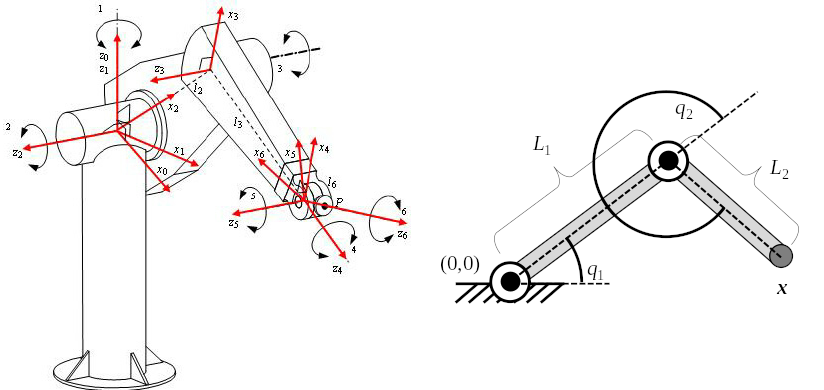
\includegraphics[width=16cm,page=1]{../img/6dof-kinematics.png}
    \caption{Pa kreisi -- tipiska 6-brīvības pakāpju industriālā robota shematisks attēls ar kinemātiskās ķēdes elementiem -- sešiem rotācijas pāriem jeb locītavām, kam katrai ir viena brīvības pakāpe \cite{harib2012parallel}. Pa labi -- apzīmējumi kinemātiskajā kēdē ar rotācijas pāriem un fiksētām nobīdēm \cite{kinematics_illinois}.}
\end{figure}

Robotu mehāniskie izpildījumi var būt ļoti dažādi, taču kopīga ir matemātisko modeļu saime, kas tiek izmantoti, lai attēlotu to izpildmehānismu tiešā veidā nomērāmos stāvokļus -- locītavu leņķus, bīdes pāru lineāros pārvietojumus -- telpiskajā (Dekarta) koordinātu telpā un otrādi. Tos dēvē par kinemātiskajām ķēdēm \cite{kinematics_illinois}. Kinemātiskā ķēde sastāv no savienojumu virknes, kas katrs ietver kinemātisko pāri un nobīdi. Katrs kinemātiskais pāris pieļauj kādu mainīgu cietķermeņa ģeometrisko pārveidojumu -- rotāciju un pārvietojumu -- kombināciju. Nobīde definē saiti starp diviem kinemātiskiem pāriem. Piemēram, ja divas rotācijas asis ir savienotas ar robota rokas segmentu, to attālums veido fiksētu telpisku pārveidojumu. Katram kinemātiskā pāra veidam ir t.s. brīvības pakāpju skaits, kas nosaka to, cik dimensiju vektors ir nepieciešams, lai viennozīmīgi aprakstītu šī pāra konfigurāciju.

Atkarībā no mehānisma uzbūves kinemātiskās ķēdes var būt atvērtas (ar vienu fiksētu punktu) vai slēgtas (ar diviem); virknē (katrs nākamais kinemātiskais pāris sa-vienots ar iepriekšējā pārveidotu koordinātu sistēmu) vai paralēlas (vairāki pāri savienoti ar vienu elementu un to stāvokļi ir savstarpēji neatkarīgi). Par kinemātiskās ķēdes konfigurāciju var saukt vektoru, kas apraksta visu kinemātisko pāru individuālās konfigurācijas -- rotācijas pāru jeb locītavu gadījumā (pieņemot, ka rotācija nav ierobežota) tie var būt leņķi


\begin{equation}
    \boldsymbol{\alpha} \in \mathcal{C}
\end{equation}
\begin{equation}
    \boldsymbol{\alpha} = (\alpha_1, ..., \alpha_n)
\end{equation}
, kur $n$ -- locītavu skaits, $\mathcal{C}$ -- robota locītavu konfigurāciju telpa. Tā kā darba ietvaros strādāts ar 6-asu industriālajiem manipulatoriem, ilustratīvam piemēram ir vērts izmantot tieši šādu robotu. Kinemātikas kontekstā pamatā tiek strādāts ar diviem uzdevumiem -- tiešo un inverso. Robota izpildmehānisms ir piestiprināts pie kinemātiskās ķēdes pēdējā elementa, un parasti nepieciešams pārveidot pozīcijas no šīs pārvietojamās koordinātu sistēmas uz robota pamatnes -- apkārtējās vides -- fiksēto. Tiešās kinemātikas uzdevums ir iegūt summāro pārvietojumu un rotāciju, ko piemērojot kādam vektoram efektora koordinātu sistēmā, var iegūt atbilstošu pārvietojuma vektoru un orientācijas reprezentāciju (sk. zemāk) globālajā koordinātu sistēmā. 

Viens no veidiem, kā definēt pārveidojumu katrā locītavā un savienojumā, ir ar pārveidojuma matricām formā

\begin{equation}
    T_{l_i}(q_i) =
    \begin{bmatrix}
        \multicolumn{3}{c}{\multirow{3}{*}{$R(\boldsymbol{a_i},\alpha_i)$}} & \multirow{3}{*}{$L_i$} \\
        \multicolumn{3}{c}{} & \multirow{3}{*}{} \\
        \multicolumn{3}{c}{} & \multirow{3}{*}{} \\
        0 & 0 & 0 & 1
    \end{bmatrix}
\end{equation}
, kur $\alpha_i$ -- locītavas leņķis (mainīgais parametrs), $\boldsymbol{a_i}$ -- rotācijas ass vienības vektors savienojuma koordinātu sistēmā (ap to tiek piemērota rotācija), $L_i$ -- pārvietojums uz nākamo atskaites punktu (3-dimensionāls vektors). $R(\boldsymbol{a_i},\alpha_i)$ ir $3 \times 3$ telpiskā rotācijas matrica, kas atbilst rotācijai ap doto asi pa doto leņķi. Tā kā šie ir lineāri pārveidojumi, tos var kombinēt

\begin{equation}
    T_{n}(\boldsymbol{\alpha}) = T_{l_n}(\alpha_n)T_{l_{n-1}}(\alpha_{n-1})...T_{l_{1}}(\alpha_{1})
\end{equation}
un piemērot pārvietojuma vektoram gala efektora koordinātu sistēmā ar matricu reizināšanu

\begin{equation}
    \boldsymbol{x}_{world} = T_{n}(\boldsymbol{\alpha})\boldsymbol{x}_{ee}
\end{equation}

Summāro rotāciju attiecīgi apzīmē kombinētās pārveidojuma matricas rotācijas \newline komponente augšējā kreisajā stūrī, ko iespējams izteikt Eilera leņķos vai citādi. Viens populārs veids, kā apzīmēt rotācijas 3-dimensiju telpā, ir izmantojot kvaternionus \cite{quaternions_illinois}. Tos var uztvert kā komplekso skaitļu 4-dimen-sionālu ekvivalentu. Šī darba ietvaros padziļināti aprakstīt to algebriskās īpašības nav nepieciešams, pietiek tikai minēt, ka, lai izteiktu telpisku rotāciju, tiek izmantota t.s. versora forma

\begin{equation}
    q = w + x\boldsymbol{i} + y\boldsymbol{j} + x\boldsymbol{k}
\end{equation}
\begin{equation}
    \Vert q \Vert = \sqrt{w^2 + x^2 + y^2 + z^2} = 1
\end{equation}
, kur $w$ ir rotācijas skalārā komponente bet $x,y,z$ veidotais 3-dimensiju vektors ir paralēls atbilstošai rotācijas asij. Svarīgi ievērot, ka kaut gan kvaternions vispārīgā gadījumā ir četrdimensionāls objekts, konstantās normas nosacījums visus versorus novieto uz 3-dimensionālas hipersfēras 4-dimensiju telpā, kas nozīmē, ka telpiskām rotācijām tik un tā ir tikai 3 brīvības pakāpes -- tāpat, kā izsakot tās ar leņķiem. Kvaternioniem ir reizinājuma operācija, kam ir vienības vērtība un inversās vērtības

\begin{equation}
    qq^{-1} \equiv 1 +  0\boldsymbol{i} + 0\boldsymbol{j} + 0\boldsymbol{k}
\end{equation}

Rotāciju vektoram 3-dimensiju telpā piemēro, to papildinot ar 0 un piemērojot rotācijas operatoru.

\begin{equation}
    L_q(\boldsymbol{v} \in \mathbb{R}^3) \equiv q(0,\boldsymbol{v})q^{-1}
\end{equation}

Šādām rotācijas operācijām iespējama kompozīcija

\begin{equation}
    L_q \circ L_p (\boldsymbol{v}) = L_{qp}(\boldsymbol{v}) = (qp)(0,\boldsymbol{v})(qp)^{-1}
\end{equation}
, kas ļauj kinemātisko ķēdes konfigurācijai atbilstošo koordinātu sistēmas pārvei-dojumu aprakstīt kā rotētu nobīžu vektoru summu

\begin{equation}
    \boldsymbol{x}_{ee} = L_{q_1}(\boldsymbol{L}_1) + L_{q_2q_1}(\boldsymbol{L}_2) + ... + L_{q_n...q_1}(\boldsymbol{L}_{ee})
\end{equation}

Robota vadības programmatūras kontekstā bieži var nākties strādāt ar t.s. robota efektora pozu, kas sastāv no divām komponentēm -- efektora koordinātu sistēmas sākumpunkta nobīdes un summārās rotācijas

\begin{equation}
    \boldsymbol{x}_{position} = \boldsymbol{x}_{world}
\end{equation}
\begin{equation}
    \boldsymbol{q}_{orientation} = \prod_{i=1}^n q_i
\end{equation}

Ja tiešās kinemātikas uzdevumā nepieciešams no zināmas robota locītavu konfi-gurācijas iegūt telpisko pozīciju, tad inversā kinemātika nodarbojas ar atbilstošu locītavu leņķu piemeklēšanu konkrētai telpiskai pozīcijai \cite{inverse_kinematics_illinois}. Formāli, tipiskais inversās kine-mātikas uzdevums ir atrast $f^{-1}$ pie konkrētas orientācijas un pozīcijas (kopā -- pozas)

\begin{equation}
    f(\boldsymbol{\alpha}) \equiv \boldsymbol{x}_{desired} = 
    \begin{bmatrix}
        \boldsymbol{x}_{position} \\
        \boldsymbol{x}_{orientation} 
    \end{bmatrix}
\end{equation}
, kur $\boldsymbol{x}_{position}, \boldsymbol{x}_{orientation}$ ir pozīcijas un orientācijas ierobežojumi, kas atbilst kon-krētam pārvietojumam un orientācijai, izteikti 3-dimensionāli. Protams, iespējams izmantot arī cita veida ierobežojumus, un to skaits var būt dažāds. Atkarībā no dotā lineāri neatkarīgu ierobežojumu skaita $m$ un robota brīvības pakāpju skaita $n$, iespējamas sekojošās situācijas:

\begin{enumerate}
    \item $n > m$ -- problēma ir nepietiekami ierobežota. Ja atrisinājums pastāv (nav ārpus robota sasniedzamās darba zonas) un nav singulārs, tad atrisinājumu ir bezgalīgi daudz;
    \item $n = m$ -- problēma ir precīzi ierobežota  (tipiski 6-asu robotam 3-dimensiju telpā). Ja atrisinājums pastāv, tad to ir galīgā skaitā;
    \item $n < m$ -- problēma ir pārlieku ierobežota. Risinājums pastāv tikai punktu apakš-kopai ar samazinātu dimensionalitāti.
\end{enumerate}

Vienkāršākais veids, kā varētu aprakstīt singulārus risinājumus jeb singularitātes robotikas kontekstā, varētu būt sekojošs: tie ir punkti pozu telpā $x_{singularity}$, kuriem pēc tiešās kinemātikas piekārtotās locītavu konfigurācijas telpa $\lbrace \alpha \mid f(\alpha) = x_{singularity} \rbrace$ ir ar citu dimensionalitāti, nekā jebkurā tā topoloģisko kaimiņu kopā. Piemēram, precīzi ierobežotās problēmas gadījumā tas varētu būtu punkts, kam iespējama tikai viena atbilstoša robota konfigurācija, bet jebkurā tā kaimiņu kopā pastāv punkti ar lielāku, galīgu iespējamu konfigurāciju skaitu. Viena šādu pozīciju saime ir visas maksimāli iztaisnota robota sasniegtās pozas.

Singularitāšu pastāvēšana, vairāku vai bezgalīgi daudzu konfigurāciju pastāvēšana (gandrīz) katrai sasniedzamai pozai un nelineārās sakarības starp locītavu leņķi un efektora atrašanās vietu telpā nozīmē to, ka izmantot vienkāršus lineārus operatorus inversās kinemātikas uzdevuma risināšanai nav iespējams. Tā vietā iespējams vai nu sastādīt nelineāras vienādojumu sistēmas, kas atbilst robota ģeometrijai, vai rēķināt rezultātu ar skaitliskām metodēm. 

\subsubsection{Trajektoriju plānošana}

Ar tiešo un inverso kinemātiku vien nepietiek, lai būtu iespējams realizēt robota vadību. Pat ja zināms robota sākuma un beigu stāvoklis pozu vai konfigurāciju telpā, jebkura kustība starp tiem sastāda līknes -- gan konfigurācijā, gan pozā. Parasti abās telpās pastāv arī ierobežojumi, kas jāievēro -- robots nedrīkst sadurties ar objektiem apkārtējā vidē (absolūtās vērtības pozu telpā), tā locītavu ātrumi vai paātrinājumi (parciālie atvasinājumi konfigurāciju telpā) nedrīkst pārsniegt ierobežojumus, u.t.t. Robotikas kontekstā kustības plānošanas problēmu var izteikt kā \cite{motion_planning_illinois}

\begin{equation}
    y(s): [0,1] \rightarrow \mathcal{C}
\end{equation}
, kas piekārto katru vērtību nepārtrauktajā intervālā $[0,1]$ atbilstošai robota konfigurācijai, ar nosacījumu, ka $y(s)$ nav pārtraukuma punktu. $y(0), y(1)$ apzīmē robota sākuma un beigu stāvokļus, pārējās $s$ vērtības -- jebkuru trajektorijas punktu starp tiem.

Telpiskās pozīcijas un locītavu konfigurāciju -- kinemātiskie -- ierobežojumi nosaka atļauto apgabalu $\mathcal{F} \subseteq \mathcal{C}$, un attiecīgi

\begin{equation}
    \forall s,y(s) \in \mathcal{F}
\end{equation}

Savukārt ierobežojumus, kas attiecināmi uz $y(s)$ atvasinājumiem, sauc par dina-miskajiem. Svarīgi piebilst, ka ne vienmēr iespējams izpildīt nepārtrauktu kustību pozu telpā -- var gadīties, ka, lai nonāktu no viena punkta nākamajā, nepieciešams tāds kustības segments konfigurāciju telpā, kura $f(y(s))$ nepieder telpiskajai trajektorijai. Šādu parā-dību sauc par ``lēcienu'', un no tās ir svarīgi izvairīties, ja uzdevuma ietvaros ir svarīga pareiza kustības telpiskā ģeometrija, kā tas ir ar metieniem.


%
%
%
%
%
%
%
%
%
%
% CHAPTER 3
% CHAPTER 3
% CHAPTER 3
% CHAPTER 3
% CHAPTER 3
% CHAPTER 3
% CHAPTER 3
% CHAPTER 3
% CHAPTER 3
% CHAPTER 3
% CHAPTER 3
% CHAPTER 3
% CHAPTER 3
%
%
%
%
%
%
%
%
%

\newpage
\section{Atdarinošā mašīnmācīšanās}

Šīs nodaļas mērķis ir pārskatīt ar nozares pētniecību saistīto zinātnisko literatūru; aprakstīt galvenos sasniegtos rezultātus, gūtās atziņas katrā no tematiskajiem apakš-virzieniem. Protams, ne visus pētījumus iespējams vienkārši klasificēt pēc to piederības šeit izvēlētajām kategorijām, un daudzi varbūt tajā vispār neiederas -- taču cenšoties gūt personisku izpratni par kādu tēmu, lai motivētu tālākus pētījumus, ir svarīgi nostatīt iepriekšējus rezultātus to kontekstā. Saprast, kāpēc tieši šobrīd aktuālie pētniecības virzieni ir tādi, kādus tos varam redzēt kādā akadēmisko publikāciju datubāzē vai neseno pētījumu pārskatā.

Salīdzinot ar citām aktuālām mašīnmācīšanās pētniecības nozarēm -- piemēram, jau minēto stimulēto mācīšanos -- tieši par atdarināšanu veiktās pētniecības apjoms ir relatīvi neliels. Taču tik un tā pieejams liels skaits publikāciju, kas apraksta pētījumus ļoti dažādos virzienos. Turklāt robotika ir viens no izplatītākajiem pielietojuma mērķiem šādām metodēm, konkurējot ar datorspēļu aģentiem. Lai radītu priekšstatu par nozares pašreizējo stāvokli un tematisku dalījumu, izšķirti trīs virzieni, kas labi apraksta lielu daļu no pētījumiem par iespējām robotus apmācīt ar piemēriem:

\begin{enumerate}
    \item trajektoriju kopēšana -- mērķis ir panākt robustu, precīzu atdarināšanu ar nelielām treniņa datu kopām, ja pieejama visa nepieciešamā informācija par sistēmas stāvokli;
    \item novērojumu iegūšana, interpretācija, papildināšana -- ne vienmēr ir pieejami dati formā, ko var tiešā veidā izmantot imitējamu trajektoriju iegūšanā. Daudzi pētījumi nodarbojas tieši ar apmācībai derīgu novērojumu iegūšanu -- netiešu (piemēram, video) novērojumu pārveidošanu, labākām cilvēka-robota saskarnes metodēm, trajektorijām ar nezināmām darbībām, u.c.;
    \item atdarināšana un adaptācija, vispārināšana -- atdarinošās mācīšanās pielietojums, lai uzlabotu stimulēto, un otrādi; vispārīgu prasmju iegūšana no demonstrācijām, tūlītēja atdarināšana. Mēģinājumi panākt, ka modelis neaprobežojas tikai ar piemē-ros esošo un spēj pielāgoties. Stimulētās mācīšanās uzsākšana ļoti retinātās atalgojumu telpās.
\end{enumerate}

\subsection{Labi definētu trajektoriju kopēšana}

Pirmā, varētu teikt galvenā, taču ne vienmēr vienkāršākā problēma, ir atrast veidu, kā pieejamās ekspertu zināšanas -- robotikas kontekstā tās parasti būs pareizas trajektorijas dažādu pārvietojumu un smalku manipulācijas uzdevumu risināšanai -- tiešā veidā atdarināt. Šo procesu mēdz saukt arī par programmēšanu ar demonstrācijām (PBD -- \textit{programming by demonstration}) \cite{muench1994robot,billard2008handbook}. Idealizētā vidē ar determinētām stāvokļu pārejām un pilnīgu informāciju par tās pašreizējo konfigurāciju šis uzdevums varētu būt pat triviāls, taču praksē saskaramies ar problēmām:

\begin{enumerate}
    \item darbs notiek ar novērojumiem, nevis stāvokļiem. Pat ja pieejami, piemēram, trajektoriju ieraksti, bieži vien trūkst svarīgas informācijas (varētu būt zināma trajektorijas kinemātika, bet ne tās dinamika -- paātrinājumi, spēki);
    \item atšķirības vidē: izpildelementos -- varbūt robots ir nedaudz citāds; apkārtnē -- varbūt manipulējamo objektu masas, forma vai izvietojums ir nedaudz atšķirīgi no demonstrācijās esošajiem;
    \item ja trajektoriju ģenerējis eksperts, kam, iespējams bijusi pieejama informācija, kuras aģentam nav -- piemēram, manipulāciju veicis cilvēks ar redzi, bet robotam pieejami tikai kontakta sensori.
\end{enumerate}

Problēmas faktiski nozīmē to, ka reālā sistēmā stāvokļu pārejas nav determinētas attiecībā pret novērojumiem un darbībām. Lai labāk saprastu šos trūkumus, vispirms noderīgi ir aplūkot ``naivākos'' veidus, kā varētu imitēt piemērus. Šajā apakšnodaļā aprakstīti pētījumi, kuros uzsvars ir uz pietiekami detalizētu demonstrāciju atdarināšanas procesiem.

\subsubsection{Vienkāršas metodes}

Pirmais, ko varētu darīt, ir tiešā veidā ierakstīt trajektoriju un to atkārtot. Šī nebūt nav jauna ideja -- gandrīz visiem mūsdienu industriāliem robotiem ir pieejamas t.s. \textit{lead-through} un \textit{teach-in} programmēšanas metodes, kas ļauj fiziski un ar tālvadības ierīces palīdzību vadīt robota kustību un to ierakstīt pēcākai atdarināšanai \cite{teach_pendant}, turklāt tās parādījušās jau pašos industriālās robotikas pirmsākumos 1970os gados \cite{abb2016special}.

Tā kā trajektorijai jābūt ierakstītai tieši ar robotu, lai tā būtu atkārtojama bez papildus datizraces uzdevumu risināšanas, var paredzēt, ka dabiski radīsies zināma tendence dominēt viegli realizējamiem, bet ne garantēti optimāliem ceļiem telpā -- vieglāk ierakstīt dažus pagrieziena punktus un ļaut programmatūrai interpolēt nekā fiziski vadīt robotu visā kustības ceļā. Pie tam var parādīties neparedzēti trūkumi, pārejot no lēnas, nenoslogotas izpildes programmēšanas procesā uz ātru un noslogotu ekspluatācijā, kas apgrūtina procesu. Faktiski sākotnējais ieraksts bieži vien kalpo par starta punktu, bet, lai nonāktu pie lietojamas programmas, nepieciešams iegūto kodu koriģēt un iteratīvi pielāgot. Lai arī principā tiek izmantota demonstrācija trajektorijas iegūšanai, procesa veikšanai tik un tā nepieciešams personāls ar robotu programmēšanas prasmēm. Jau sen atzīts \cite{muench1994robot,billard2008handbook}, ka, lai tik tiešām robotus varētu apmācīt tikai ar piemēriem, nepieciešamas metodes, kas ir robustākas pret nobīdēm no paraugu ģenerējošā procesa apstākļiem un vispārināmākas, tāpēc uzsākti pētījumi ar mašīnmācīšanās metodēm.

Kad jāspēj atdarināt kas vairāk nekā viena, nemainīga trajektorija, nepieciešams atdarināt nevis pašu trajektoriju, bet gan procesu, kas tādas ģenerē -- ``eksperta'' jeb ``instruktora'' stratēģiju. Viena no vienkāršākajām metodēm, kas bieži tiek lietots kā piemērs, taču praksē reti kad ir pielietojuma, ir uzvedības klonēšana (\textit{behavioural cloning}). Vispārīgi to definēt ir samērā vienkārši \cite{attia2018global}. Ja dots MDP un kāda eksperta stratēģija $\pi^*$, kas šo MDP optimāli risina, mērķis ir atrast maksimāli tuvu modeli $\pi_{\theta}$, kur

\begin{equation}
    \pi_{\theta}(s) \approx \pi^*(s)
\end{equation}

Parasti, protams, ir pieejama datu kopa ar eksperta izietajām stāvokļu-darbību laikrindām, turklāt jāstrādā ir ar novērojumiem, nevis stāvokļiem. Lai veidotu vispārīgu izpratni par atdarinošo mašīnmācīšanos, noderīgi ir detalizētāk aplūkot kādu vienkāršu tās piemēru. Uzvedības klonēšana sistēmā, kur netiek veikta intensīva treniņa datu pārstrāde vai vadības algoritma argumentu pārveidošana, ļoti labi kalpo šādiem mērķiem, tāpēc var aplūkot 1989. gadā Kārnegija-Melona Universitātē veikto pētījumu ``\textit{Autonomous Land Vehicle in a Neural Network}'' (ALVINN) \cite{pomerleau1989alvinn}. Tā mērķis bija izstrādāt pašbraucošu automašīnu, kas spēj sekot ceļa kontūram.

Automašīna tikusi aprīkota ar videokameru un LIDAR sensoriem, kas devuši divus skatus uz to pašu telpas reģionu automobiļa priekšā. Par apmācāmo modeli izvēlēts neironu tīkls. Protams, 1989. gads vēl bija laiks, kad datoru veiktspēja bija stipri ierobežota, tāpēc neironu tīkls ir klasiskas uzbūves -- tam ir viens slēptais slānis ar 29 perceptroniem, kam seko 45 izvades elementi. Video izmantots krāsainā attēla zilais kanāls, jo tajā ceļa virsma visvairāk kontrastē ar apkārtējo vidi. Gan video, gan LIDAR radītie attēli tīkla ievadē veido vienkāršu vektoru bez nekādiem telpiskiem kodējumiem, visi slāņi savstarpēji pilnībā savienoti.

\begin{figure}[t!]
    \centering
    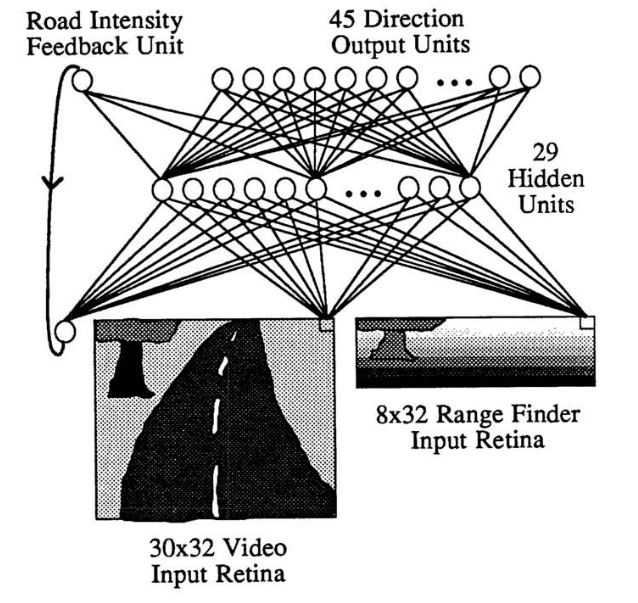
\includegraphics[height=6.8cm,page=1]{../img/alvinn_architecture.png}
    \caption{ALVINN modeļa uzbūve \cite{pomerleau1989alvinn}}
\end{figure}

Modeļa izvades slānis apzīmē vēlamo stūrēšanas virzienu 45 diskrētos soļos. Treniņa datu kopā faktisko virziena komandu atspoguļo neprecizēta veida ``zvana'' funkcija ar modu pie pareizā virziena. Ieviests viens papildus perceptrons, kas (teorētiski) novērtē ceļa gaišumu, salīdzinot ar apkārtējo vidi, un tiek pievienots nākamās iterācijas ievades vektoram. Konstatēts, ka ievākt treniņa datus fizikālā vidē -- braucot ar automašīnu pa ceļiem un ierakstot vadītāja veiktās korekcijas -- nav praktiski, jo nepieciešama ļoti liela treniņa datu kopa. Tāpēc dati ģenerēti sintētiski -- tā kā gan video, gan attāluma datu izšķirtspēja ir gaužām neliela, pat ar 1989. gadā pieejamām datorgrafikas iespējām šādi gūtus attēlus ir grūti atšķirt no īstiem. Simulatorā iegūtie attēli un vadības komandas izmantoti klasifikatora apmācībā.

Iegūtais rezultāts -- modelis, kas bijis pietiekami labs, lai spētu vadīt ar kameru un attāluma sensoru aprīkotu automobili pa 400m garu slēgta ceļa posmu saulainos dienas apstākļos, ar ātrumu 0,5m/s. Kā galvenais uzvedības klonēšanas trūkums parasti tiek minēta nespēja atgūties no faktiskā stāvokļa sadalījumu nobīdes \cite{attia2018global} (\textit{distribution shift}). Ja reālais modelis $\pi_{\theta}(s)$ nevar pilnīgi precīzi atdarināt eksperta $\pi^*(s)$ darbības vai MDP pārejas funkcija ir stohastiska, tātad treniņa datu kopa neietver visas iespējamās trajektorijas ar atbilstošajām $\pi^*(s)$ vērtībām, $\pi_{\theta}$ inducētais stāvokļu sadalījums diverģē no $\pi^*$ inducētā. Lai iegūtu precīzāku un robustāku eksperta stratēģijas atdarinājumu, piedāvāti dažādi -- sarežģītāki -- apmācības paņēmieni.

\subsubsection{Statistiskas korekcijas}

Viens no virzieniem, kurā veikti mēģinājumi uzlabot trajektoriju kopēšanas lietderību, ir strukturēt treniņa datu ieguvi un apmācības algoritmu veidā, kas maksimāli tuvina $\pi^*$ un $\pi_{\theta}$ inducētos stāvokļu sadalījumus. Bieži vien tas nozīmē, ka vienkārši ievākt datus un veikt apmācību uz tiem vairs nav iespējams -- nepieciešama aktīva instruktora iesaiste. Piedāvātie risinājumi ir dažādi, un metodes var kļūt visnotaļ sarežģītas \cite{attia2018global}, tāpēc, lai ilustrētu pieejas būtību kopumā, izvēlēts viens, vairāk teorētisks piemērs.

DAgger -- \textit{dataset aggregation} -- ir 2011. gadā publicētajā rakstā ``\textit{A Reduction of Imitation Learning and Structured Prediction
to No-Regret Online Learning}'' \cite{ross2011no}, piedāvāts algoritms. Tas pierāda teorētiskas garantijas $\pi^*$ un $\pi_{\theta}$ inducēto sadalījumu konverģencei, kombinējot instruktāžu ar apmācāmā modeļa ģenerētām stratēģijām. Lai gan raksts nav tieši saistīts ar robotiku, izmantotais MDP kontroles formālisms ir vispārīgs.

Algoritma darbību var vienkāršoti aprakstīt sekojoši: pieņem, ka ir pieejami ne tikai eksperta ģenerēti trajektoriju dati, bet ir iespējams pašam ekspertam uzdot vaicājumus par katrā stāvoklī optimālu darbību -- kas, ja instruktāžu nodrošina cilvēks un laika soļu pārejas ir biežas, reti kad būs praktiski iespējams. Tādā gadījumā iteratīvi atkārto šādus soļus:

\begin{enumerate}
    \item ar kādu varbūtību $\alpha$ izvēlas, vai i-tā trajektorija tiks ģenerēta ar $\pi^*$ vai $\pi_{\theta}$;
    \item iegūtās laikrindas stāvokļa elementiem $s_t$ atrod atbilstošo $a^*_t=\pi^*(s_t)$ 
    \item kopējai datu kopai $D$ pievieno $D_i=\lbrace (s_1, a^*_1),... \rbrace$
    \item apmāca modeli $\pi_{\theta}$ uz papildinātās datu kopas
\end{enumerate}

Kā jau minēts, liela daļa raksta satura veltīta tieši algoritma teorētisko īpašību pierādīšanai, taču beigās arī veikti daži eksperimenti -- divi ar personāžu vadību dator-spēļu vidē, viens ar rokraksta zīmju atpazīšanu teksta virknēs. Lai gan visos gadījumos DAgger pārspēj uzvedības klonēšanas (vienkāršas $\pi^*$ aproksimēšanas no treniņa datu kopas) rezultātus, tā lietderību stipri ierobežo instruktora interaktivitātes prasības -- praksē reti kad ir iespējams kaut kas analoģisks datorspēļu aģentu treniņam izmantotajam simulatoram, kas ar dziļu pārlasi atrod labas stratēģijas jebkuram stāvoklim.

\subsubsection{Inversā stimulētā mācīšanās}

Cits veids, kā atdarināt instruktora dotas trajektorijas, ir pieņemt, ka tā stratēģija optimizē kādu slēptu atalgojuma funkciju $R^*(s)$ un mēģināt to atjaunot no pieejamās informācijas. Šādā veidā ar stimulētās mašīnmācīšanās metodēm var iegūt meklēto rezultā-tu. Kā jau parasti, iespējami dažādi veidi, kā formalizēt uzdevumu un tehniski to realizēt. 2004. izdotais ``\textit{Apprenticeship learning via inverse reinforcement learning}'' \cite{abbeel2004apprenticeship} no Džordžijas Tehnoloģiju institūta, viens no citētākajiem rakstiem par šo tēmu (lai arī ne pirmais), piedāvā iteratīvu algoritmu nezināmas atalgojuma funkcijas atjaunošanai un izmantošanai. Galvenā atkāpe no tipiska MDP formālisma ir pieņēmums, ka nezināmā atalgojuma funkcija $R^*$ ir formā

\begin{equation}
    R^*(s) = w^* \cdot \phi(s)
\end{equation}
, kur $w^*$ -- svaru vektors, bet $\phi: S \rightarrow [0,1]^k$ -- zināmu atribūtu izpausme noteiktos stāvokļos. $\phi$ nozīme ir tāda, ka ir iespējams noteikt, kādu sakarību lineāra kombinācija varētu būt īstā atalgojuma funkcija. Kā piemērs tiek piedāvāts autovadītāja uzdevums -- viens no atribūtiem varētu būt 1, ja mašīna atrodas uz ceļa, bet 0 citādi, u.t.t. $m$ treniņa kopas trajektorijām aprēķina vidējo faktoru vērtību summu, izteiktu kā

\begin{equation}
    \mu^* = \frac{1}{m}\sum_{i=1}^m\sum_{t=1}^T \gamma^t \phi(s^i_t)
\end{equation}

Tad tiek iteratīvi atkārtota procedūra, kur atrod kādu svaru vektoru $w^{i}$ un attiecīgi empīrisku atalgojuma funkciju $R^{i}(s) = {w^{i}}^T\phi(s)$, ko izmanto, lai apmācītu jaunu stratēģiju $\pi^i$. Tad šai stratēģijai atrod vidējo vērtību $\mu^i$ analoģiski (2.3), un visas iepriekšējās $\mu^{j \leq i}$ tiek izmantotas, lai atrastu nākamo svaru vektoru $w^{i+1}$. Process turpinās, līdz ir konverģējis līdz noteiktam kļūdas hiperparametram. Tādējādi beigās iegūta stratēģija, kas maksimizē līdzīgu atribūtu $\phi(s)$ kombināciju nezināmajai instruktora stratēģijai, un robusti seko demonstrācijām.

Rezultāti parāda, ka šī metode pārspēj dažādas vienkāršas, statistiskas $\pi^*$ aproksi-mācijas metodes (uzvedības klonēšanu). Kopā risināti divi dažādi uzdevumi. Viens ir ``\textit{gridworld}'' -- spēle, kurā aģents pārvietojas pa režģa formas vidi un dažos lauciņos ir pieejams atalgojums. Taču pārejas process ir stohastisks, tāpēc metodes, kas atdarina tikai telpiskos pārvietojumus un nemēģina atjaunot slēpto atalgojuma funkciju darbojas sliktāk. Otrs ir divdimensionāla spēle, kurā aģents vada automobili. Šeit tika pārbaudīts, vai var iemācīt aģentam atšķirīgus ``braukšanas stilus'' tikai ar demonstrācijām, kas arī izdevies.

\subsubsection{Ģeneratīvie pretinieku tīkli}

Iedvesmojoties no inversās stimulētās mācīšanās, attīstītas arī citas metodes, kas tiešā vai netiešā veidā nodarbojas ar instruktora stratēģijas aproksimēšanu. Bieži kā trūkums IRL metodēm tiek minēta nepieciešamība katrai iteratīvi iegūtajai stratēģija no jauna veikt stimulēto apmācības procesu, lai būtu iespējams iegūt šīs metodes ģenerētas trajektorijas un līdz ar to varētu novērtēt to sasniegto stāvokļu atribūtu sadalījumus. Meklējot veidus, kā tiešā veidā optimizēt stratēģiju, lai tā sasniegtu tādus pašus novērtē-jumus kā demonstrācijas pie plašām iespējamo atalgojuma funkciju klasēm, izlaižot pašu šo atalgojuma funkciju meklēšanu, 2016. gadā publicēts ``\textit{Generative Adversarial Imitation Learning}'' \cite{ho2016generative}. Tas piedāvā risināt trajektoriju atdarināšanas uzdevumu ar pretinieku tīklu metodi, un ir bijis samērā ietekmīgs uz tālākiem pētījumiem nozarē, jo šobrīd tā jau ir visai populāra metode, un vēl salīdzinoši nesen tika uzskatīta par labāko tieši trajektoriju kopēšanas uzdevumā \cite{torabi2018generative}.

\begin{figure}[t!]
    \centering
    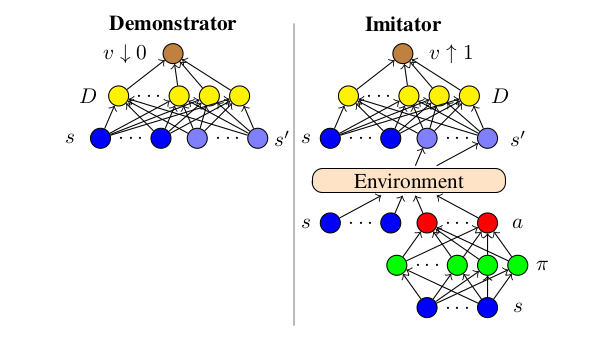
\includegraphics[height=7cm,page=1]{../img/GAN.png}
    \caption{GAN uzbūves piemērs. Augšējais tīkls -- diskriminators -- cenšas atšķirt eksperta demonstrācijas no ģeneratora radītām trajektorijām \cite{torabi2018generative}}
\end{figure}

Ģeneratīvie pretinieku tīkli -- GAN, \textit{generative adversarial networks} -- tiek apmācīti ar metodi, kas ļauj izmantot adaptīvu mērķa funkciju. Tā vietā, lai optimizētu visu modeli vienam mērķim, tiek izdalīti divi elementi -- ģenerators un diskriminators -- ar pretējiem uzdevumiem. Diskriminators ir klasifikators, kas apmācīts atšķirt demonstrāciju kopas trajektorijas vai to elementus no visām pārējām. Ģenerators no sistēmas stāvokļiem vai novērojumiem ģenerē darbības tā, lai diskriminators nebūtu spējīgs atšķirt tās no parauga. Formāli pierādījumi šī modeļa konverģencei ir pārāk apjomīgi, lai tos apskatītu šajā darbā. Tomēr no augstāk minētā pētījuma un citiem tā iedvesmotajiem rakstiem, kas aprakstīti zemāk, var secināt, ka pēc sekmīgas abu modeļu apmācības būs iegūta stratēģija, kas tuvu aproksimē ievades datu sadalījumu.

\subsubsection{Uzdevumu simboliska dekompozīcija}

Vēl viena metode atdarināšanas spēju uzlabošanai ir telpisku kustības trajektoriju pārvēršana simbolisku, diskrētu darbību virknē. Pamatideja ir tāda, ka vieglāk iemācīties robusti izpildīt primitīvas kustības un tad šādu primitīvo kustību secību kāda uzdevuma izpildē, nekā no neliela demonstrācija skaita iemācīties katru uzdevumu pilnībā no jauna. Šī arī nebūt nav jauna ideja -- izteikta jau 1980os un 1990os gados \cite{muench1994robot}. Jau 2002. gadā veikti pētījumi par algoritmiem, kas ļauj aproksimēt trajektorijas elementus ar autonomu nelineāru diferenciālvienādojumu sistēmām \cite{ijspeert2002movement} un iemācīt pietiekami sarežģītas kustības -- piemēram, tenisa bumbas sišanu -- ar samērā nedaudziem piemēriem (ap 20). Ap to pašu laiku piedāvātas arī pieejas šādu primitīvu kustību kombinēšanai \cite{schaal2003computational}, kur mašīnmācīšanās lietojums attiecināts ne tikai uz atsevišķajiem trajektorijas primitīviem, bet arī uz katrai demonstrācijai atbilstošas to secības meklēšanu.

Robotikas literatūrā pirms 2010. gada \cite{billard2008handbook} plaši rakstīts par šādiem paņēmieniem, taču pēdējos gados aizvien biežāk tiek izmantotas metodes, kuru pamatā ir vispārīgāki neironu tīklu modeļi. Jebkurā gadījumā, aktīva pētniecība nozarē vēl joprojām notiek, it sevišķi pielietojumiem, kur robots tiek mācīts ar kinestētiskām metodēm. Piemēram, ``\textit{A Framework of Hybrid Force/Motion Skills Learning for Robots}'' \cite{wang2020framework}, kas publicēts 2020. gadā, šāda pieeja tiek veiksmīgi izmantota uzdevumiem, kur svarīga ne tikai telpiskā trajektorija, bet arī uz apkārtējo vidi izdarīto spēku profils (galda virsmas tīrīšanā).

\subsection{Novērojumu iegūšana, interpretācija, papildināšana}

Pat ja demonstrācijas ir iespējams ļoti precīzi atdarināt, praksē paveras jauna prob-lēma -- ne vienmēr iespējams tiešā veidā iegūt pietiekami labus paraugus no instruktoriem. Ja novērojums $o_t$ ir netiešs -- iegūts formā, kas neatbilst robota vadības algoritmam nepieciešamajam sistēmas konfigurācijas aprakstam -- to nepieciešams pārveidot. Turklāt, darbojoties ar netiešiem novērojumiem, bieži vien tiešā veidā iespējams atjaunot tikai stāvokļu $s_t$ laikrindu -- darbības $a_t$ paliek nezināmas.

Strādājot apstākļos, kur vienkārši analītiski modeļi ar labu precizitāti var paredzēt stāvokļa atribūtus un sakarības starp tiem, šī atšķirība var nebūt īpaši svarīga. Piemēram, darbojoties ar robotu, kas nav sevišķi smagi noslogots un kura kontroles sistēma spēj bez lielām novirzēm atdarināt no tās prasīto kinemātiku, var ar augstu precizitāti darboties ar novērojumiem, kuros zināmi tikai šie kinemātiskie atribūti. Tas varbūt pat ir vienkāršāk, nekā izmantot smalkāku konfigurācijas aprakstu, kur pieejami arī visi dinamikas atribūti. 

Taču daudziem potenciāli ļoti noderīgiem lietojumiem galvenais šķērslis apmācībai var būt tieši derīgu treniņa datu kopu iegūšana no nepilnīgiem novērojumiem. Problēmas var sagādāt demonstrāciju ģenerēšana ar citādas ģeometrijas instruktoru (piemēram, cil-vēku), citu objektu sarežģītu un iepriekš nezināmu konfigurāciju modelēšana (manipulē-jamo objektu novietojums, orientācija, u.t.t.), trajektoriju automātiska iegūšana no datu kopām, kas nav tiešā veidā paredzētas šim mērķim (video ieraksti). Tāpat jāpārvar zināmi izaicinājumi, lai datus varētu ģenerēt ar netiešām metodēm -- piemēram, attālinātu vadību vai virtuālās realitātes simulācijām.

\subsubsection{Nezināmas darbības}

Pētījumos, kuru galvenā būtība ir dažādu veidu pārveidojumi ar kinemātiskiem vai dinamiskiem trajektoriju datiem, varētu teikt, ka uzsvars ir uz kinestētiskajiem mācīšanās aspektiem. Iepriekšējā apakšnodaļā aplūkoto eksperimentu veicēji pārsvarā pieņēmuši, ka pieejami pareizi formatēti dati, kuros novērojuma atribūti ir cieši saistīti ar robota vadībai svarīgiem sistēmas atribūtiem un zināmas katrā trajektorijas solī veiktās darbības. Savukārt šajā tiek apskatīti gadījumi, kad dati ir kādā ziņā nepietiekami vai pārveidoti.

Pirmais sarežģījums, ko varētu ieviest, ir darbību trūkums demonstrācijās. Ar to jāsastopas ļoti daudzos uzdevumos -- no nemarķētiem datiem var vienkārši iegūt, piemēram, robota gala efektora pozīciju un rotāciju, taču nekas nav zināms par tā locītavu leņķiskajiem paātrinājumiem. Lai varētu izmantot jau zināmos atdarinošās mācīšanās algoritmus, rodas nepieciešamība uzminēt attiecīgās darbības, kas noved pie pārejas no viena stāvokļa uz nākamo.

``\textit{Behavioral Cloning from Observation}'' \cite{torabi2018behavioral} (2018) ir viena šāda metode. Tās mērķis ir realizēt jau aprakstīto uzvedības klonēšanas algoritmu laikrindu datiem, kuros pieejami tikai novērojumi. Lai to panāktu, tiek ieviests papildus modelis, tikai šoreiz nevis stratēģijas, bet gan paša robota (vai cita aģenta) dinamikas aproksimēšanai.

Nedaudz vienkāršojot, algoritma soļi ir sekojoši:

\begin{enumerate}
    \item doto trajektoriju kopu pārveido formā $\mathcal{T}_{dem}=\lbrace (s_t, s_{t+1}) \rbrace$, kas ir pārejas starp stāvokļiem;
    \item stratēģija $\pi_{\theta}$ un sistēmas dinamikas modelis $M_{\phi}(a \vert s,s')=P(a \vert s, s')$ tiek nejauši inicializēti;
    \item ģenerē trajektorijas ar $\pi_{\theta}$, pievieno trajektorijas elementus kopai $\mathcal{T}=\lbrace (s_t, a_t, s_{t+1}) \rbrace$;
    \item apmāca $M_{\phi}(a \vert s, s')$ uz $\mathcal{T}$;
    \item trenē $\pi_{\theta}$ uz $\lbrace (s_t, \operatorname*{argmax}\limits_a M_{\phi}(a \vert s, s'), s')\vert (s, s') \in \mathcal{T}_{dem} \rbrace$
    \item atkārto soļus 3-5 līdz sasniegti pieņemami rezultāti
\end{enumerate}

Redzams, ka pakāpeniski tiek iegūts sistēmas slēptās dinamikas modelis, kas pareizi paredz pārejas funkcijas darbības parametru, un, tāpat kā parastajā gadījumā, tiek apmācīta atbilstoša stratēģija. Interesanti arī, ka šajā situācijā potenciāli nedaudz lielāks uzsvars ir tieši uz nākamo novērojumu laikrindā, nevis izvēlēto darbību -- pie $s$, $\pi_{\theta}$ iemācās paredzēt \textit{s' sasniegšanai labāko darbību}, nevis vienkārši atkārtot pašu darbību bez konteksta, tātad savā ziņā sistēmas dinamika un vēlamais rezultāts tiek ņemti vērā. Rezultātos autori salīdzina šo metodi ar citām, kas izmanto arī darbību datus no demonstrācijām, un konstatē, ka šis algoritms pat strādā labāk nekā tās, ja tiek vērtēts pēc nepieciešamo demonstrācijas trajektoriju vai simulācijas iterāciju skaita.

Iepriekšējā apakšnodaļā 2. attēls ir no ``\textit{Generative Adversarial Imitation from Observation}'' \cite{torabi2018behavioral} (2018), kas turpina darboties tajā pašā virzienā, tikai šoreiz ar GAN modeļa palīdzību. Tā vietā, lai modelētu sistēmas dinamiku, diskriminators klasificē trajektoriju laikrindās sastopamās stāvokļu pārejas $(s, s')$ pēc tā, vai tās būtu sastopamas demonstrācijā, bet ģenerators (kas reizē ir arī stratēģija $\pi_{\theta}$) tiek trenēts, lai tā izvēlēto darbību rezultātā iegūtās stāvokļu pārejas $s=T(s,a)$ nebūtu atšķiramas no piemēriem.

\subsubsection{Dinamikas novērojumu iegūšana, izmantošana, vispārināšana} 

Cita veida problēma, kas arī prasa korekciju ieviešanu, ir atdarināšana sistēmām ar mainīgu dinamiku. Robotiem izmantojot ``\textit{lead-through}'' programmēšanas metodi, kustības tiek programmētas bez slodzes un, iespējams, neievērojot ātrumu -- zināma tikai daļēja sistēmas kinemātika. Ja var paredzēt, ka pēc tam ekspluatācijā atšķirsies robotu slogojošie spēki un griezes momenti, tad var meklēt veidus, kā šīs novirzes treniņa datu ieguves procesā kompensēt. ``\textit{Online Movement Adaptation based on Previous Sensor Experiences}'' \cite{pastor2011online} (2011) paredz jau iepriekš aprakstīto simboliskās dekompozīcijas modeļu papildināšanu ar korekcijām reālā laikā, izmantojot atgriezenisko saiti ar gan paša robota iekšējiem devējiem, gan ārējiem sensoriem. 

Pētījumos, kas nodarbojas ar simbolisko dekompozīciju, bieži vien tiek aprakstīti visai sarežģīti un tieši robotu dinamikai specifiski matemātiskie modeļi. Taču vienkāršoti procesu var aprakstīt sekojoši: kustības raksturojošie diferenciālvienādojumu modeļi tiek iegūti, robotu manuāli vai citādi pārvietojot. Tad kustība tiek veikta ar pareizu kinemā-tiku (ātrumiem, paātrinājumiem), bet bez papildu slodzes. Tiek ierakstīti sensoru novēro-jumi un veidoti kustībai atbilstoši modeļi, kas paredz šos raksturlielumus trajektorijas gaitā. Autoru vārdiem -- robots iemācās, kā kustībai vajadzētu ``justies''. Tad reāli ekspluatācijā var sekot līdzi nobīdēm no normas un ar klasiskās kontroles teorijas metodēm veikt korekcijas.

Nodarbojoties ar ļoti sarežģītiem uzdevumiem (piemēram, salikšanas procesiem), mēģināt vadīt robotu cauri visiem iespējamajiem detaļu savstarpējiem stāvokļiem var būt neiespējami. Ja var iegūt demonstrācijas kādā citā, vieglāk realizējamā veidā un izstrādāt vispārīgu metodi, kā tos atdarināt neatkarīgi no robota uzbūves, rodas iespējas automatizēt arī šādus procesus. ``\textit{Contact Skill Imitation Learning for Robot-Independent Assembly Programming}'' \cite{scherzinger2019contact} (2019) realizē šādu procedūru, izmantojot divus būtiskus elementus:

\begin{enumerate}
    \item \textit{forward dynamics compliance control} -- robota vadības algoritmu, kurā tiek kontrolēti uz efektoru iedarbojošos spēku un griezes momentu vektori, nevis izpildelementu pozīcija \cite{scherzinger2017forward};
    \item rekurentos neironu tīklus laikrindas nākamā elementa paredzēšanai -- t.i., tīklus, kuru ievadē parādās iepriekšējā laika soļa izvades vektors no tā paša modeļa;
\end{enumerate}

Demonstrāciju iegūšanai cilvēks simulācijas vidē ar datorpeles palīdzību veic salikšanas procesu, izmantojot tikai vizuālo uztveri un intuitīvu izpratni par sadursmju dinamiku. Novērojumus veido manipulējamā objekta masas centrā reģistrēto griezes momentu un spēku vektori. Stratēģija -- rekurentais neironu tīkls -- $\pi_{\theta}$ tiek apmācīta paredzēt nākamo spēku/momentu vektoru laikrindā, un tas tiek izmantots robota kontrolei ar minēto vadības algoritmu.

\subsubsection{Demonstrācijas no cilvēka darbībām}

Ja nepieciešams ātri un lēti radīt treniņa datu kopas apmācības procesiem -- kā tas  būtu praktiski izmantojamai robotu programmēšanas sistēmai -- svarīgi radīt cilvēkam draudzīgu saskarni. Tā vietā lai programmētu robota trajektoriju ar tradicionālām meto-dēm, ir veikti mēģinājumi attīstīt paņēmienus, kas ļautu dabiski ierakstīt cilvēka izpildītas kustības un izteikt tās formā, ko var izmantot robota apmācībai. Viens no virzieniem, kurā veikta izpēte, ir tieša fiziskās kinemātikas ierakstīšana un pārveidošana. ``\textit{Imitation learning in industrial robots: a kinematics based trajectory generation framework}'' \cite{jha2017imitation} (2017) ir piemērs šādam pētījumam. Tiek izmantota \textit{Microsoft Kinect} -- savulaik populāra, videospēļu vadībai paredzēta kustību uztveres ierīce, kas spēj ierakstīt kāda objekta kustību aprakstošu punktu virkni telpā -- lai ierakstītu cilvēka kustības. Tad ar analītiskām metodēm tiek veikta trajektoriju interpolācija, grupēšana ar klasterizācijas algoritmu, un izpildē vēlamo trajektoriju ieguve ar tuvāko kaimiņu metodēm.

Lai mazinātu atšķirības starp cilvēkam un robotam pieejamām novērojumu un darbību telpām, var izmantot virtuālo realitāti -- gan simulācijās, gan robota tālvadībai. ``\textit{Deep imitation learning for complex manipulation tasks from virtual reality teleoperation}'' \cite{zhang2018deep} (2018) ir aprakstīta fiziska robota tālvadības sistēma, kas robota novēroto vidi pārveido sintētiskā telpā, kur cilvēks var ar manipulatoru palīdzību intuitīvi vadīt robota kustības. Šis uzdevums nav gluži triviāls, jo jāpārvar atšķirības starp, piemēram, robota kameras un cilvēka galvas kustību ātrumu, lai neradītu diskomfortu lietotājam. Tādējādi iegūta demonstrāciju datu kopa, kas sastāv no attēliem un telpiskiem dziļumiem, ko arī tālāk var izmantot konvolūciju neironu tīklā, lai realizētu uzvedības klonēšanu.

\subsubsection{Video demonstrācijas, perspektīvu pārbīde}

Ļoti plašas iespējas demonstrāciju iegūšanai radītu spēja tās iegūt no video datiem un izmantot šādas ``redzes'' sistēmas arī tiešā vadības uzdevuma risināšanai. Izrādās, ka daži no jau iepriekš aplūkotajiem algoritmiem ir pietiekami vispārīgi, lai tos varētu pielāgot šim uzdevumam. Piemēram, GAN no novērojumiem \cite{torabi2018generative} ir ļoti robusts attiecībā pret ievades datu formu un saturu, ja vien tajos ir iespējams pietiekami labi atšķirt demonstrāciju no citām trajektorijām. Tāpat kā gadījumā, kad strādā ar kinemātiku aprakstošiem stāvokļiem, GAN vienkārši tiek apmācīts diskriminēt/ģenerēt trajektoriju vizuālās reprezentācijas, ar samērā labiem rezultātiem.


Brīdī, kad vairs netiek izmantoti robota konfigurāciju aprakstoši novērojumi, rodas jauna problēma -- iegūtie novērojumi ir atkarīgi no izmantotās perspektīvas, kas vispārīgā gadījumā var arī nesakrist ar robota vadības algoritmu ievades datus ģenerējošo. ``\textit{Imitation from observation: Learning to imitate behaviors from raw video via context translation}'' \cite{liu2018imitation} (2018) risina šo atšķirīgo kontekstu sarežģījumu un iegūto modeli izmanto arī rezultātu uzlabošanai kopumā. Pieņemot, ka trajektorijai atbilstošie novērojumi tiek iegūti no dažādām perspektīvām telpā, vispirms tiek apmācīts enkodera-dekodera tipa neironu tīkls, kas iegūst novērojumu vektoriālas reprezentācijas, ko pēc tam iespējams dekodēt par tai pašai sistēmas konfigurācijai atbilstošu novērojumu no jebkuras perspektīvas. Tas ļauj ne tikai tiešā veidā ``tulkot'' novērojumus no vienas kameras uz citu, bet arī izmantot iegūtās kodētās reprezentācijas Eiklīda distanci no demonstrāciju trajektoriju soļiem atbilstošajām kā atalgojuma funkciju stimulētās mašīnmācīšanās algoritmam. Arī intuitīvi skaidrs, ka modelis, kas spēs atjaunot situācijas attēlu kādā perspektīvā, ja zināmi tikai no citas perspektīvas gūtie attēli, kaut kādā ziņā sevī ietver visus nozīmīgos konfigurācijas atribūtus.

\subsubsection{Datu sintēze, telpiski modeļi}

\begin{figure}[t!]
    \centering
    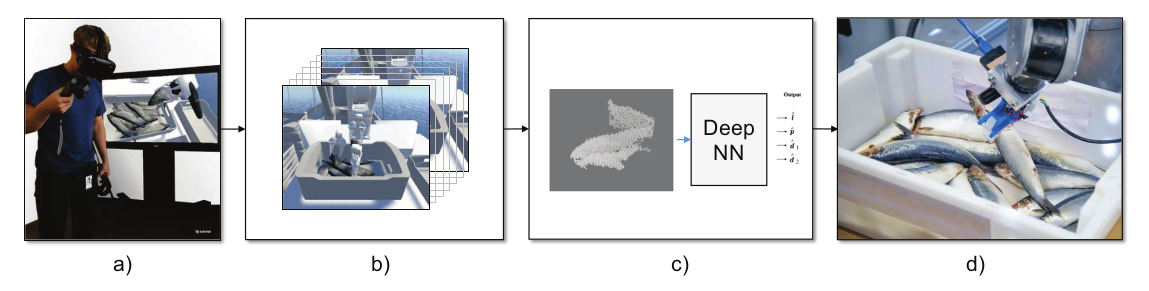
\includegraphics[width=16cm]{../img/fish.png}
    \caption{Zivs satveršanas modeļa apmācība: a) cilvēka radīto demonstrāciju iegūšana; b) datu kopas sintētiska pavairošana; c) telpiska konvolūciju neironu tīkla apmācība; d) veiksmīga zivs satveršana realitātē. \cite{dyrstad2018teaching}}
\end{figure}

Daudzi uzdevumi, kam tiek izmantoti roboti, sevī ietver manipulāciju ar citiem objektiem, kuru telpisko novietojumu un citus atribūtus ne vienmēr viegli iegūt, un nākas paļauties uz netiešiem novērojumiem, ko sagādā, piemēram, datorredzes sistēmas. Ja objekti ir paredzamā orientācijā un regulāras formas, no šīs problēmas parasti iespējams izvairīties, taču vēl joprojām daudzi pārvietošanas un pozicionēšanas procesi tiek veikti ar cilvēka roku darbu.

``\textit{Teaching a robot to grasp real fish by imitation learning from a human supervisor in virtual reality}'' \cite{dyrstad2018teaching} ir labs piemērs šāda tipa pētījumam, kura ietvaros izstrādāts modelis zivju satveršanas uzdevumam. Robotam ir jāspēj no kastes, kurā atrodas vairākas zivis, satvert un pārvietot vienu. Risinājuma pamatā ir trīs idejas:

\begin{enumerate}
    \item zivs pozīcijai un orientācijai piemērota satveršanas punkta un leņķa paredzēšana, izmantojot ar telpisko kameru gūtus punktu mākoņa datus. Tam pielieto konvolūciju neironu tīklu -- izmantojot vispārinātas metodes, kas sākumā izmantotas divdimensionāla attēlu klasifikācijai;
    \item demonstrāciju ievākšana virtuālās realitātes vidē, kas ļauj cilvēkam viegli un dabiski ģenerēt satvērienus;
    \item datu kopas sintētiska pavairošana.
\end{enumerate}

Novērojumi gūti, cilvēkam VR vidē brīvā veidā satverot zivis dažādos veidos. Lai viennozīmīgi aprakstītu katru iespējamo satvērumu, izmantoti trīs vektori -- pozīcija (punkta), garenās ass orientācija un rotācija ap to.  Pēc tam ģenerēts liels skaits zivju izvietojuma konfigurāciju. Lai sintētiskie dati būtu lietojami, nepieciešams nodrošināt, ka satvēruma matrica tiek koriģēta atbilstoši zivs izliekumam, novietojumam un orientācijai. Katrā sagatavotajā sistēmas konfigurācijā katrai zivij sākumā piešķirti visi iespējamie satvēruma vektori, no kuriem atsijāti visi, kas kolīziju dēļ nav sasniedzami. Šie dati tad izmantoti 3-dimensionālā konvolūciju neironu tīkla apmācībai -- simulatorā ģenerēti ainai atbilstoši telpiskie attēli, modelis apmācīts kā tipisks klasifikators.

\subsection{Atdarinošu modeļu vispārināšana un adaptācija}

Ja pieejamas demonstrācijas no eksperta, to atdarināšana tiešā veidā varbūt ir pirmais solis noderīgu stratēģiju iegūšanā, taču nebūt ne vienīgais, ko iespējams darīt. Līdz šim aplūkotas metodes, kas izrāda zināmu adaptācijas pakāpi, lai precīzāk un robustāk imitētu paraugus, taču vienmēr izdarīts pieņēmums, ka instruktors kādā ziņā optimāli izpildījis uzdevumu. Turklāt visos gadījumos, lai apmācītu sistēmu izpildīt jaunu uzdevumu, nepieciešams veikt intensīvu treniņu ar cilvēka starpniecību. 

Šajā apakšnodaļā aprakstīti pētījumi, kuros meklēti veidi, kā apvienot atdarināšanu ar adaptāciju, lai vispārinātu demonstrācijās ietverto informāciju, atvieglotu jaunu uzdevumu programmēšanas procesu vai pārspētu instruktoru sasniegto rezultātu kvalitātē. Lai gan iespējams atrast desmit gadus un vairāk senus pētījumus, kuros, piemēram, izmantotas sarežģītas un tieši robotikas mērķiem specifiskas simboliskās dekompozīcijas metodes \cite{pastor2011skill} -- uzsvars šeit tiek likts uz nesenākām un vispārīgākām metodēm, kas attīstītas jau pašreizējā neironu tīklu uzplaukuma periodā.

\subsubsection{Neoptimālu demonstrāciju uzlabošana}

Jau pati atdarinošās mācīšanās pamatnostādne -- apgūt stratēģiju problēmas risi-nāšanai, pēc iespējas tuvāk sekojot kādai demonstrāciju kopai -- sevī ietver pieņēmumu par demonstrācijas optimalitāti. Taču izrādās, ka iespējams pašu treniņa datu kopu izmantot, lai gūtu informāciju par to, ko instruktors patiesi vēlējies sasniegt, un attiecīgi optimizēt modeli šī slēptā mērķa sasniegšanai.

``\textit{Extrapolating beyond suboptimal demonstrations via inverse reinforcement learning from observations}'' \cite{brown2019extrapolating} (2019) izmanto jau iepriekš aprakstīto inversās stimulētās mācīšanās algoritmu saimi par pamatu jaunai metodei. Tā vietā, lai atrastu atalgojuma funkciju, kas pamato demonstrāciju kopas trajektorijas $\tau$, tiek meklēta tāda, kas skaidro to \textit{sakārtojumu}. Tāpēc nepieciešams datu kopu papildināt ar kārtojumu $\prec$, lai

\begin{equation}
    \tau_i \prec \tau_j \Rightarrow \sum_{s_t \in \tau_i}R(s) \leq \sum_{s_t \in \tau_j}R(s)
\end{equation}

Protams, kārtojums var arī nebūt ideāls -- trajektoriju vērtējums var būt subjektīvs vai trokšņains, ja nav zināma īstā atalgojuma funkcija, tāpēc jārēķinās ar kļūdainu pāru attiecību pastāvēšanas iespējamību ar kļūdas varbūtību $\epsilon$

\begin{equation}
    \exists \epsilon \geq 0 : \tau_i \prec \tau_j \Rightarrow P\left(\sum_{s_t \in \tau_i}R(s) \leq \sum_{s_t \in \tau_j}R(s)\right) = 1 - \epsilon
\end{equation}

Ja kārtojums ir pieejams, radoši nosauktais \textit{Trajectory-ranked Reward EXtrapolation} jeb T-REX algoritms darbojas divos soļos:

\begin{enumerate}
    \item izmantojot demonstrāciju datus, tiek apmācīta nezināmās atalgojuma funkcijas $R(s)$ aproksimācija $r_{\phi}(s)$ -- parametrisks modelis, konkrēti neironu tīkls;
    \item tāpat kā IRL gadījumā, rekonstruētā atalgojuma funkcija tiek izmantota, lai apmā-cītu stratēģiju $\pi_{\theta}$ ar stimulētās mašīnmācīšanās metodēm.
\end{enumerate}

Eksperimentāli pārbaudīts, ka piemēros, kur zināmas demonstrācijām atbilstošās īstās atalgojuma funkcijas un kļūdas varbūtība saglabājas zem 15\%, rekonstruētā atalgojuma funkcija $r_{\phi}$ daudzos gadījumos labi aproksimē īsto. Turklāt, ja izmantotās demonstrācijas nav optimālas, iegūtā stratēģija $\pi_{\theta}$ tās pārspēj.

\subsubsection{Demonstrācija -- sākumpunkts apmācību procesam}

Atšķirībā no IRL un augstāk aprakstītā T-REX, ir iespējams uz atdarinošās un stimulētās mācīšanās kombināciju skatīties arī no otras puses -- nevis izmantot stimulētās metodes, lai realizētu atdarināšanu, bet gan izmantot demonstrācijas, lai uzlabotu parasto stimulētās mašīnmācīšanās procesu ar zināmu atalgojuma funkciju.

``\textit{Deep Q-learning from demonstrations}'' \cite{hester2018deep} (2018) piedāvā vispārīgu metodi stimu-lētās mācīšanās procesa inicializācijai ar demonstrāciju datu kopas palīdzību. Šādu pieeju motivē viens no lielākajiem klupšanas akmeņiem RL algoritmu apmācībā -- ja atalgojuma funkcijas nenulles vērtības konfigurāciju telpā ir stipri retinātas, kā tas ļoti bieži ir arī dažādos robotikas uzdevumos, tad, praktiski apmācot stratēģiju izpildīt tai uzdoto uzdevumu, nepieciešams ļoti liels skaits treniņa soļu -- lai šo telpu apstaigātu, atrastu vēlamos rezultātus un optimizētu trajektoriju caur tai.

Q-mācīšanās gadījumā stratēģiju var uzdot formā $\pi_{\epsilon Q_{\theta}}$ ar $\epsilon, Q_{\theta}$ tā, ka

\begin{equation}
    T(s,a) = P(s'\mid s,a) \rightarrow Q_{\theta}(s,a) \approx \mathbb{E}[v(s')] 
\end{equation}
-- t.i, modelis $Q_{\theta}$ aproksimē matemātisko cerību atalgojumam attiecībā iespējamām darbībām (jeb nākamo stāvokļu vērtības) $v(s')$ -- un attiecīgi izvēlas vienu darbību pēc ``$\epsilon$-alkatīgas'' stratēģijas

\begin{equation}
    a = 
    \begin{cases}
        \operatorname*{argmax}_a Q(s,a) \text{ ar varbūtību } 1-\epsilon; \\
        \text{ nejauši izvēlēta no iespējām ar varbūtību } \epsilon
    \end{cases} 
\end{equation}

Demonstrācijas tad tiek izmantotas, lai apmācītu $Q_{\theta}$ vēl pirms notiek jebkāda modeļa mijiedarbība ar vidi, un attiecīgi tas jau uzreiz darbojas daudz kvalitatīvāk nekā nejauši inicializēts modelis. Rezultāti liecina, ka jau sākotnējās iterācijās šāds algoritms var darboties visai labi, kas paver iespējas to izmantot situācijās, kad nav iespējams veikt apmācību simulācijas vidē, bet ir pieejami demonstrāciju dati. Robotikas kontekstā tas nozīmē, ka, ja jāveic apmācība uz fiziska robota, modeļa sagatavošana ar atdarināšanu varētu būt visai noderīgs paņēmiens.


\subsubsection{Tūlītēja trajektoriju atdarināšana}

Līdz šim aplūkotās atdarinošās metodes darbojas ar pieņēmumu, ka mērķis ir no demonstrāciju datu kopas iegūt modeli, kas pēc apmācības spēj izpildīt vienu uzdevumu, un attiecīgi treniņa algoritms neparedz iespēju bez papildus iterācijām atdarināt iepriekš neredzētas demonstrācijas -- tipiski pieejams tikai pašreizējais sistēmas stāvoklis ievadē un vēlamā darbība izvadē.

Salīdzinot ar bioloģiskām sistēmām, uzreiz ir skaidrs, ka šādi procesi nekad nespēs izdarīt cilvēkam šķietami pašsaprotamo -- novērot darbību un uzreiz to atkārtot bez liela skaita treniņa iterāciju. Lai būtu iespējams sasniegt šādu rezultātu, ir nepieciešams nevis modelis, kas ar paraugiem ticis optimizēts vienas stratēģijas atdarināšanai, bet gan tāds, kas vispārina pašu atdarināšanas procesu -- ievadē sistēmas pašreizējais stāvoklis tiek apvienots ar demonstrāciju, lai iegūtu vēlamo darbību. 

``\textit{One-Shot Imitation Learning}'' \cite{duan2017one} (2017) šādu rezultātu sasniedz, apmācot sarež-ģītas uzbūves modeli, kas apmācīts no vienas demonstrācijas paredzēt citas vispārīgā veidā. Tā ievades vektors satur veselu treniņa kopas trajektoriju. Modelis tiek apmācīts uzreiz veselai līdzīgu uzdevumu kopai, nevis tikai vienam konkrētam.

Konkrēti, pētītā uzdevumu saime ir kubisku detaļu kraušana vienai uz otras ar robotu. Novērojumu ģenerēšanas un interpretēšanas problēmas gan tiek apietas, jo sis-tēmas stāvokli raksturojošie vektori satur gan robota iekšējo konfigurāciju, gan detaļu relatīvās pozīcijas attiecībā pret robota efektoru. Tad, izmantojot konvolūciju un uzmanības mehānismus, dažādu garumu trajektoriju laikrindas tiek reducētas uz vienu sistēmas stāvokļa vektoru, kas paredz piemērotāko darbību attiecībā pret doto demonstrāciju un momentāno sistēmas stāvokli.

\subsubsection{Nestrukturētas demonstrācijas, plānu veidošana no galamērķiem}

Droši vien lielākā atkāpe no ``klasiskā'' atdarinošā mašīnmācīšanās uzdevuma ir tajos pētījumos, kur tiek atmests pieņēmums, ka ir dotas diskrētas parauga trajektorijas ar zināmu uzdevumu. Tā vietā pat pārraudzītā trajektoriju marķēšanas stadija tiek automatizēta un atstāta apmācības algoritma pārziņā. Tā vietā var novērot, ka, ja mērķis ir iemācīties modeli, kas spēj vispārīgi atrast ceļu no vienas sistēmas konfigurācijas uz citu, pietiek atrast trajektorijas, kuras satur abas. ``\textit{Learning Latent Plans from Play}'' \cite{lynch2020learning} (2019) ierosina demonstrāciju strukturētas ievākšanas vietā izmantot cilvēka dabisko tendenci spēlēties ar dažādiem objektiem, lai virtuālās realitātes vidē ģenerētu demonstrāciju kopas. Sistēma šajā gadījumā ir virtuālā realitātē modelēta vide, bet pieejamie novērojumi -- robota iekšējā konfigurācija un simulēti attēli.

Lai no šādas nestrukturētas informācijas iegūtu praktiski izmantojamas stratēģijas, nepieciešams papildināt stratēģijas formālismu ar mērķa jēdzienu -- ne vairs vienkārši atrodot katram stāvoklim piekārtotu $\pi(s)$, bet gan parametrizētu pēc vēlamā beigu stā-vokļa (\textit{goal}) -- $\pi(s,s_{g})$. Ja pieejamas trajektoriju laikrindas formā $s_1, s_2, ..., s_n$, nav grūti pamanīt, ka jebkura apakšvirkne veido sākuma-gala stāvokļu pāri ar visām to starpā esošajām pārejām.

Tiek piedāvāti divi dažādi modeļu šabloni un apmācības algoritmi, kas spētu iegūt reālas stratēģijas no nestrukturētu datu kopas. Pirmais modelis $\pi_{\theta}(s,s_g)$ saņem ievadē pašreizējo un vēlamo stāvokli, un paredz nepieciešamo darbību. Kā šablons tiek izmantots rekurentais neironu tīkls, treniņa datus veido trajektorijas, un pēdējais trajektorijas stāvoklis kļūst par $s_g$. $\pi_{\theta}$ optimizē, lai katram $(s_t, a_t, s_g)$ būtu $\pi_{\theta}(s_t, s_g) \approx a_t$. Taču pastāv problēma -- var pastāvēt dažādas trajektorijas starp jebkuriem $s, s_g$, kas draud apgrūtināt apmācības procesu.

Otrs, sarežģītākais modelis apkaro šo parādību, modelējot plāna jēdzienu -- tiek pieņemts, ka katrai trajektorijai $\tau$ var piekārtot rīcības plānu, visiem iespējamiem rīcības plāniem pastāv vektoriālas reprezentācijas $z$, un vieglāk ir vispirms paredzēt atbilstošāko plānu, pēc tam -- piemeklēt tam viennozīmīgi piekārtotu trajektoriju. Modelis tad sastāv no trim daļām:

\begin{enumerate}
    \item plānu enkodera $q_{\phi}(z \vert \tau)$, kas izsaka trajektorijas ar matemātisko cerību un standartnovirzi vektoriem $\mu_{\phi}, \sigma_{\phi} = q_{\phi}(\tau)$;
    \item plānu selektora $q_{\psi}(z \vert s, s_g)$, kas analoģiski paredz $\mu_{\psi}, \sigma_{\psi} = q_{\psi}(s, s_g)$ un iegūst no sadalījuma konkrētu vektoru $z$ diferencējamā veidā (pieskaitot vidējām vērtībām gadījuma lieluma reizinājumu ar standartnovirzi);
    \item dekodera $\pi_{\theta}(z, s, s_g)$, kas rekonstruē nepieciešamo darbību no plāna reprezentācijas, galamērķa un sistēmas momentānā stāvokļa.
\end{enumerate}

Divi varbūtību sadalījumi $q$ nepieciešami, jo optimizācijas procesā tiek minimizēta Kulbaka-Leiblera diverģence starp tiem -- ļaujot visu trajektoriju aizstāt ar tikai diviem tās punktiem. Otrs mērķa funkcijas faktors ir kļūda darbībā $a_t$. Tā kā visi slāņi ir diferencējami, viss modelis kopā veido vienu neironu tīklu, ko kopā arī apmāca uz trajektoriju apakšvirknēm. Stratēģija ir $\pi_{\theta}(q_{\psi}(s, s_g), s, s_g)$.

Tātad, lai programmētu robotu izpildīt kādu konkrētu uzdevumu, vairs nav nepieciešamas ne papildus treniņa iterācijas, ne demonstrācijas -- pietiek norādīt vēlamo sistēmas gala stāvokli, un stratēģija to pati sasniegs. Secināts, ka šāda mācīšanās pārspēj klasisko uzvedības klonēšanas metodi 18 dažādiem uzdevumiem.

Interesants turpinājums šim pētījumam ir ``\textit{Language conditioned imitation learning over unstructured data}'' \cite{lynch2021language}, kur iegūtais veikta vēl viena uzdevuma inversija -- ja pastāv metode, kas spēj pati izdalīt uzdevumus un grupēt tos pēc būtības, tad apvienojot to ar sagatavotiem marķējumiem, var iegūt stratēģiju, kas vadāma ar šādiem marķējumiem. Konkrēti, ja daļai no trajektorijām tiek \textit{a posteriori} piekārtots dabiskā valodā izteikts mērķis, var apmācīt modeli, kas sasaista rīcības plānu reprezentācijas ar frāžu reprezen-tācijām -- ļaujot vadīt robotu ar jau iepriekš apmācītu valodas enkoderu ģenerētiem kodiem. Praktiski tas izpaužas tā, ka iespējams robotam dot pavisam dabiskas komandas, turklāt neatkarīgi no izvēlētajiem sinonīmiem un pat dažādās valodās.

Ar tīri atdarinošām metodēm iegūtas stratēģijas var nebūt optimālas, it sevišķi gadījumos, kad tiek prasīts sasniegt mērķi, kam nav sagatavota speciāla demonstrāciju datu kopa. ``\textit{Relay policy learning: Solving long-horizon tasks via imitation and reinforcement learning}'' \cite{gupta2019relay} (2019) piedāvā apvienot nestrukturētas demonstrāciju datu kopas un galamērķus kā uzdevuma specifikāciju ar zināmu atalgojuma funkciju. Tā varētu iegūt labas inicializācijas apmācības procesiem, kas citādi būtu nepraktiski vai teju neiespējami ar vienkāršām konfigurāciju telpas pārstaigāšanas metodēm to retināto atalgojuma vērtību dēļ.

\subsubsection{Ļoti lielu, vispārināmu laikrindu regresoru pielietošana}

Sekojot līdzi tikai literatūrai, kas uzsver tieši atdarinošās un stimulētās mašīn-mācīšanās nozarē pielietotās terminoloģijas lietojumu, būtu viegli palaist garām problemātikas ziņā tuvu radniecīgus rezultātus, kuru autori līdz tiem nonākuši no citu nozaru pētniecības. MDP formālisms tā klasiskajā formā izslēdz dažādus sarežģītāka izpildījuma autoregresorus, kaut gan tiem iespējams piemeklēt visnotaļ produktīvus pielietojumus arī atdarināšanas uzdevuma risināšanā.

Pavisam nesen radusies iespēja šo darbu papildināt ar pavisam jaunu, ļoti aktuālu publikāciju no \textit{DeepMind}. \textit{``A Generalist Agent''} ir 2022. gada 12. maijā pirmspublikācijā izplatīts raksts, kura pamatā ir viena laikrindu autoregresora pielietojums dažāda veida sekvenciālu datu atdarināšanai, tai skaitā -- atdarinošajam uzdevumam robotikā \cite{reed2022generalist}.

\begin{figure}[t!]
    \centering
    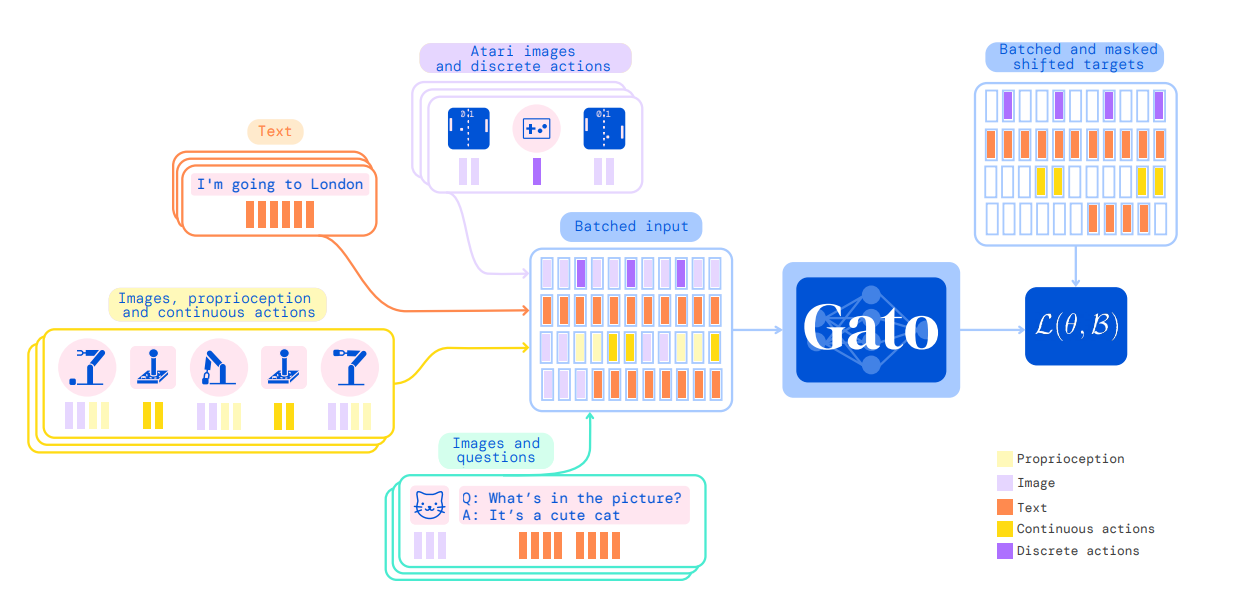
\includegraphics[width=16cm,page=1]{../img/gato.png}
    \caption{\textit{Gato} -- vispārināms atdarināšanas aģents, kas ar vienu un to pašu transformatora modeli spēj paredzēt radikāli dažādu sistēmu vektorizētu reprezentāciju laikrindas \cite{reed2022generalist}.}
\end{figure}

Izmantotais modelis ir t.s. transformers jeb pašuzmanības tīkls -- pirmo reizi pie-dāvāts šobrīd jau ļoti slavenajā 2017. gada rakstā \textit{``Attention is all you need''} kā risinājums teksta virkņu tulkošanas un autoregresijas uzdevumiem \cite{vaswani2017attention}. Tā ir modulāra neironu tīkla arhitektūra, kas sastāv no potenciāli daudziem līdzīgiem transformeru blokiem, kuram katram ir klasisku neironu tīklu un uzmanības mehānisma elementi. Šādus modeļus ar ļoti lieliem parametru skaitiem pēdējo gadu laikā veiksmīgi izmanto dažādu dabiskās valodas apstrādes uzdevumu risināšanā, kur tie pakāpeniski aizstāj vēl nesen populārās rekurentās tīklu arhitektūras \cite{radford2018improving}.

Konkrētajā pētījumā dažādu modalitāšu ievaddati tiek pārveidoti atbilstošos semantisko marķieru vektoros (\textit{``tokens''}), kas pēc tam tiek attēloti modeļa ievadā izmantotajā vektoru telpā ar apmācāmu iegulšanas modeli. Tiek nodalīti novērojumu marķieri un darbību marķieri. Modelis tiek darbināts kā autoregresors un paredz visus marķierus ievada virknē, taču mērķa funkcija tiek piemērota tikai ``darbībām'' -- teksta autoregresijas gadījumā tie būtu visi izvadītie marķieri, jo katrs atbilst apakšvārda iegultai formai, bet robotu vadības uzdevumā daļa no marķieriem atbilst novērojumam un daļa -- darbībai. Atkarībā no uzdevuma problemātikas, novērojuma un darbības reprezentācijai var atbilst dažādu garumu marķieru virknes. Par to rekonstrukciju izmantojamā formā atbild katram uzdevumam atsevišķa dekodera sekcija, kas ir inversā operācija iepriekš aprakstītajai marķieru kodēšanai un attēlošanai vektoru telpā. Robotu vadības kontekstā apmācībai izmantotas iepriekš sagatavotu stimulētās mācīšanās modeļu sagatavotas demonstrācijas, kas padara šo par klasisku atdarinošās mācīšanās uzdevumu. 

Rezultāti liecina, ka šāds modelis ļoti veiksmīgi apgūst ekspertu stratēģijas un sasniedz augstus novērtējumus, piemērojot to apmācībā izmantotās atalgojuma funkcijas -- kaut gan pats atdarinošais modelis apmācības procesā tās neizmanto. Tas vieš pārliecību, ka laikrindu paredzēšanas modeļi ir perspektīvs virziens tālākai atdarinošo metožu attīstībai.



%
%
%
%
%
%
%
%
%
%
% CHAPTER 5
% CHAPTER 5
% CHAPTER 5
% CHAPTER 5
% CHAPTER 5
% CHAPTER 5
% CHAPTER 5
% CHAPTER 5
% CHAPTER 5
% CHAPTER 5
% CHAPTER 5
% CHAPTER 5
% CHAPTER 5
%
%
%
%
%
%
%
%
%

\newpage
\section{Praktiskā realizācija}

Šī maģistra darba ietvaros aptuveni 4 mēneši pavadīti EDI robotikas un mašīn-uztveres laboratorijā, nodarbojoties ar motivējošā uzdevuma praktiska risinājuma mek-lēšanu un izstrādi. Rezultātā ar kustības uztveršanas metodēm ierakstītas demonstrāciju datu kopas, veikta to priekšapstrāde un pārveidošana neironu tīklu apmācībai derīgā formātā, apmācīti vairāku veidu modeļi pie dažādiem hiperparametriem, veikta to autoregresijas procesā ģenerēto trajektoriju ierakstīšana, vizualizācija un darbināšana uz robota -- gan simulācijas vidē, gan uz fiziskas aparatūras.


\subsection{Izmantotie rīki, aprīkojums un platformas}

Robotikā tiek integrētas tehnoloģijas no ļoti daudzām nozarēm, tāpēc lietoto rīku ietekme uz darbības virzienu ir ļoti jūtama. Tas, kurus no iepriekšējā nodaļā aprakstī-tajiem teorētiski iespējamajiem risinājumiem ir iespājams realizēt praksē, ir atkarīgs no pieejamā aprīkojuma un citiem resursiem, tāpēc svarīgi iezīmēt kontekstu, kādā attīstīta darba praktiskā daļa.

\subsubsection{ROS}

Viens no Robotikas un mašīnuztveres laboratorijā veiktās pētniecības stūrakmeņiem ir atvērtā koda \textit{``Robot Operating System''} (turpmāk -- ROS) platforma \cite{ros_org}. Par spīti nosaukumam, tā ir nevis operētājsistēma, bet gan programmatūras pakotņu kopums, kas paredzēts tiražējamai dažādu robotikas problēmu risināšanai. Šie rīki pieejami pamatā \textit{Linux} saimes operētājsistēmās, turklāt īpaši pielāgoti \textit{``Ubuntu LTS''} versijām. Līdzīgi kā \textit{Python} programmēšanas valodā, šobrīd platforma tiek izplatīta vecākajā ROS1 un jaunākajā, nesaderīgajā ROS2 versijā. Laboratorijā vēl joprojām tiek lietota platformas pirmā versija, tāpēc par to arī tālāk runāts.

Varētu teikt, ka ROS platformas pamatfunkcija ir starpprocesu komunikācijas mehā-nisma nodrošināšana, kam piedāvāti trīs dažādi paveidi \cite{ros_comm_patterns}:

\begin{enumerate}
    \item Tematu-abonentu modelis (\textit{``topics''}) -- paredzēts nepārtrauktu datu plūsmu organizēšanai. Nenoteikts skaits publicētāju, kas jebkurā brīdī var saziņas kanālā publicēt stingri noteikta formāta ziņojumu. Abonenti ir procesi, kas reģistrē atzvanīšanas funkcijas datu saņemšanai. Nav nekādas plūsmas kontroles, un ziņojumi var ``izkrist'' bez nekādām iespējamām korekcijām;
    \item Pakalpojumu modelis (\textit{``services''}) -- paredzēts momentāniem ārēju funkciju izsaukumiem, kurus nav iespējams pārtraukt. Klienta-servera modelis, kur klienta process uzsāk komunikāciju;
    \item Darbību modelis (\textit{``actions''}) -- paredzēts garāku darbību izpildei, kur nepieciešams sekot līdzi procesa stāvoklim. Arī realizēts kā klienta-servera saziņas process, taču šoreiz jau ar sarežģītāku galīgo automātu, kas nosaka savstarpējo komandu un informācijas apmaiņas modeli, un paredz iespēju ar ārēju izsaukumu pārtraukt (\textit{``preempt''}) uzsāktu darbību.
\end{enumerate}


\begin{figure}[t!]
    \centering
    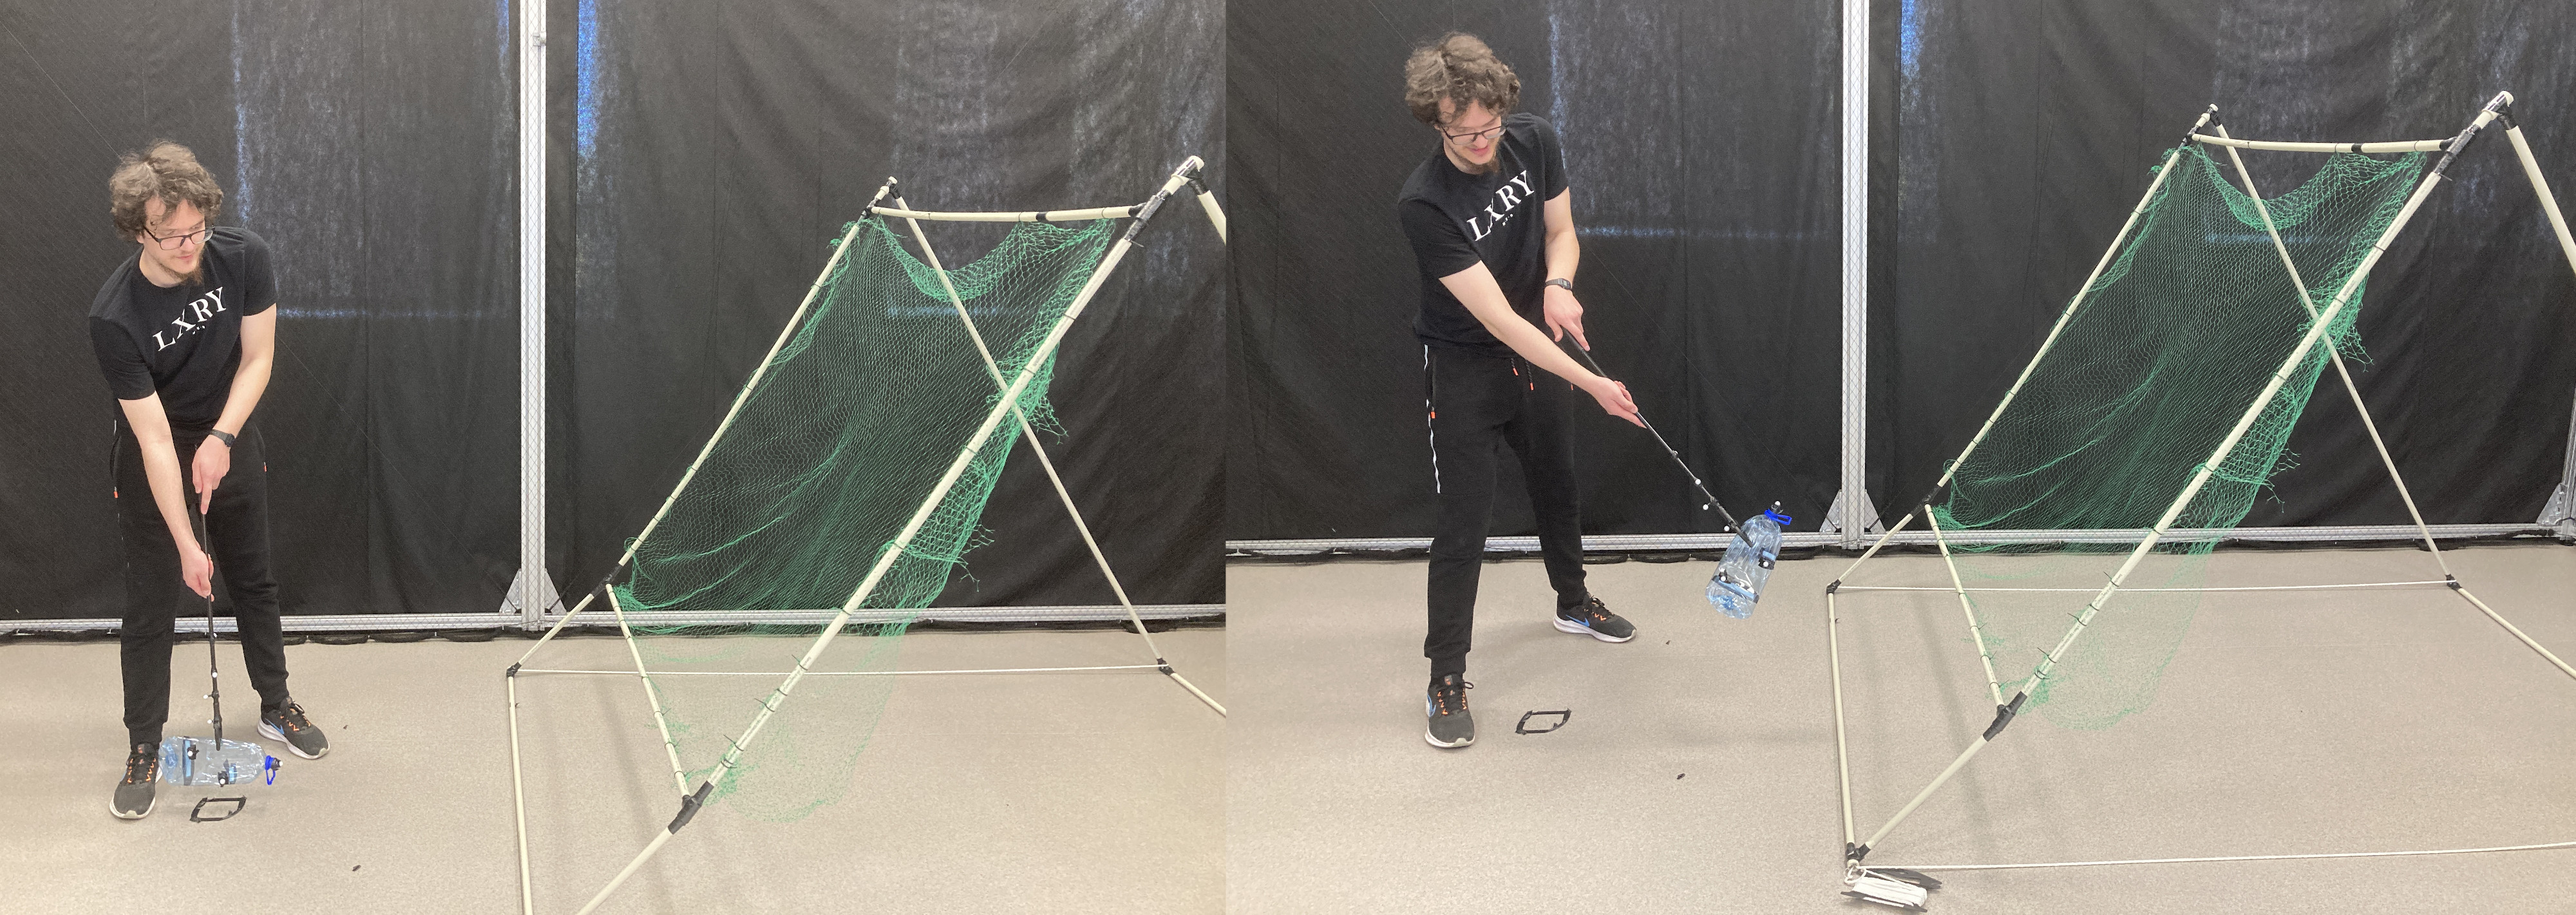
\includegraphics[width=16cm,page=1]{../img/throw_demo.jpg}
    \caption{Demonstrāciju ievākšana kustības uztveres sistēmā \textit{Optitrack}. Robota efektoru simulē atkritumu savākšanas instruments. Tīkls izgatavots, lai netiktu bojāti marķieri uz pudeles.}
\end{figure}

Papildus šai pamatinfrastrukūrai, ROS nodrošina arī pakotņu kompilācijas un instalācijas sistēmu, kā arī ļauj ar vides mainīgo un lietotņu palīdzību viegli apvienot dažādu ROS pakotņu izsaukumus lietotāja skriptos. Pakotnes tiek izstrādātas kā \textit{C++} un/vai \textit{Python} lietojumprogrammas. To izsaukumi tiek kontrolēti ar speciāliem XML formāta palaišanas failiem (\textit{``Launch Files''}), bieži vien vienlaicīgi izsaucot daudzas izpildāmās programmas ar dinamiski konfigurētiem parametriem \cite{roslaunch_file}. \textit{C++} programmatūras izstrādei pieejamas daudzas bibliotēkas, kam parasti ir arī automātiski ģenerētas \textit{Python} saskarnes.

Apjomīgākās lietojumprogrammas, kas izmantotas šī darba ietvaros, ir telpisku objektu vizualizācijas rīks \textit{rviz}, laikrindu datu kopu attēlotājs \textit{plotjuggler}. Bet saskarni ar robotiem nodrošina to ražotāju izstrādātie robotu dziņi un vairāki abstrakcijas slāņi virs tiem -- no kuriem nozīmīgākais ir \textit{MoveIt}, kas nodrošina darbību serveri saziņai ar robotu dziņiem. Jāpiemin, ka arī kustību uztveres sistēma \textit{Optitrack} piedāvā iespēju saņemt reālā laikā straumētos odometrijas datus ar ROS tematu -- tā tie arī ierakstīti.

\subsubsection{Optitrack -- aprīkojums un programmatūra}

Laboratorijā pieejams \textit{Optitrack} kustību uztveres aprīkojums, kas izmantots demonstrāciju trajektoriju ieguvei. Sistēma sastāv no 8 kamerām, kas nosaka īpašu, ļoti atstarojošu marķieru pozīciju telpā. Lai varētu izsekot kādu objektu, nepieciešams tam piestiprināt pietiekami daudzus šādus marķierus, lai jebkurā iespējamā orientācijā vairākas kameras spētu viennozīmīgi identificēt konkrēto ķermeni un triangulēt tā pozu. Kaut gan ROS kontekstā pieņemts jebkādi novērotas un rekonstruētas ķermeņa pozas datus apzīmēt ar terminu ``odometrija'', jāpiebilst, ka šis termins gan īstenībā ir attiecināms tikai uz braucošu iekārtu pozīcijas aprēķinu, integrējot to riteņu leņķiskos pārvietojumus \cite{odometry}.

Saskarni ar kustību uztveres aprīkojumu nodrošina ražotāja izplatītā \textit{Motive} programmatūras pakotne, kas gan pieejama tikai operētājsistēmā \textit{Windows}. Tāpēc nepie-ciešama atsevišķa darbstacija šim mērķim, un iegūtie dati tiek straumēti iekšējā tīklā. Lai šiem straumētiem datiem varētu piekļūt ar tematu metodi ROS vidē tiek izmantota ROS pakotne \textit{mocap\_optitrack}, kas publicē saņemtās datu paketes kā tematu ziņojumus. Ziņojumu ierakstīšanu realizē ar ROS lietotni \textit{rosbag}, kas visus tematā publicētos ziņo-jumus apkopo izvaddatu failā.

Demonstrāciju ievākšanas mērķiem izstrādāti vairāki fiziski darbarīki, kas redzami 7. attēlā. Pirmkārt nepieciešams reģistrēt pozīciju kādam ķermenim, kas kalpo kā robota efektora simulators. Lai ķermeni būtu iespējams izsekot, tam jābūt nemainīgas formas, un tā unikālais marķieru izvietojums jāreģistrē \textit{Motive} lietojumprogrammā (redzams 7. attēlā, pa labi). Turklāt attālumiem starp marķieriem būtu jābūt pietiekami lieliem, lai tie varētu kalpot objekta atpazīšanai. Tāpēc marķieru stiprināšana pie cilvēka rokas tika noraidīta kā potenciāls rīcības plāns. 

\begin{figure}[t!]
    \centering
    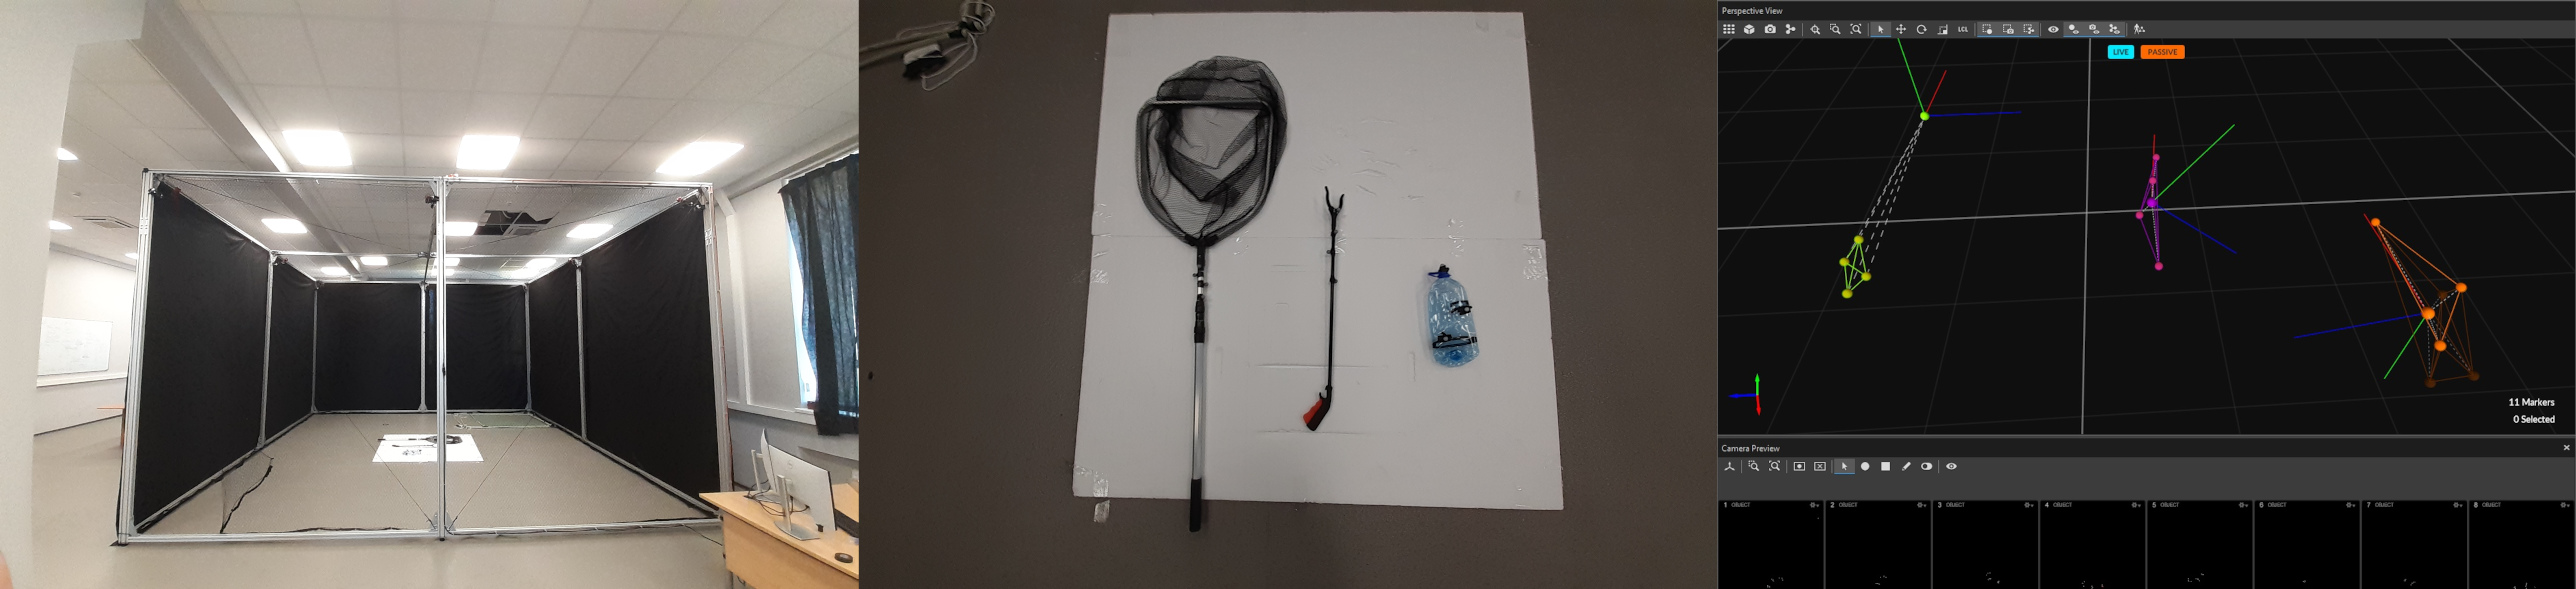
\includegraphics[width=16cm,page=1]{../img/mocap_equipment.jpg}
    \caption{No kreisās puses: \textit{Optitrack} aprīkojuma būris; ar marķieriem aprīkotie rīki -- pirmais tīkls (izmantots kā lidojuma beigu atskaites punkts), efektora simulators, pudele; cietu ķermeņu definīcijas \textit{Motive} programmatūras vidē.}
\end{figure}

Tā vietā tika atrasts instruments, kas tuvu aproksimē robota satvērējmehānisma darbību un aprīkots ar marķieriem. Tas pats darīts ar plastmasas pudeli. Lai varētu izdarīt metienus, nesalaužot marķierus, nepieciešams noķert pudeli. Sākumā izmantots neliels makšķerēšanas tīkls, taču zemās mešanas precizitātes dēļ ar to iespējamo metienu attālums ir visai neliels. Turklāt iespējamo trajektoriju dispersija ir neliela. Tā vietā izgatavots vēl viens, daudz lielāks tīkls pudeles ķeršanai. Mazais tīkls bijis aprīkots ar marķieriem, lai būtu iespējams noteikt pudeles pozīciju relatīvi tam datu priekšapstrādes procesos. Tāpēc to turpināts izmantot šiem mērķiem arī ar lielo tīklu, vienkārši novietojot to vēlamajā attālumā uz grīdas. Trajektoriju ierakstīšanas process ilustrēts 6. attēlā, kur redzama viena metiena izpilde.

\subsubsection{Programmēšanas valoda, bibliotēkas}

Datu priekšapstrādes, modeļu apmācības, robota vadības, veiktspējas novērtējuma mēru un trajektoriju vizualizāciju iegūšanai galvenokārt izmantota programmēšanas valoda \textit{Python}. Pamatā izmantotā tās versija ir 3.8+, kas savietojama ar jaunāko ROS1 platformas versiju (paredzētu \textit{Ubuntu LTS 20.04} operētājsistēmai). Taču robota vadības mērķiem daļa koda pārnesta uz \textit{Python 2.7}, jo to izmanto vecāka ROS1 versija, kas uzstādīta uz robotu kontrolei paredzētās darbstacijas.

Datu korpusi projekta ietvaros saglabāti \textit{.csv} -- \textit{``comma-separated values''} -- formāta failos, un to apstrādei lielākoties izmantota bibliotēka \textit{pandas} \cite{pandas_docs}. Tā sniedz iespēju viegli lasīt un rakstīt \textit{.csv} formāta failus, pārveidojot tos par \textit{DataFrame} objektiem atmiņā. \textit{DataFrame} ir abstrakcija, kas ļauj ar dažādu tipu informāciju saturošiem divu dimensiju datu korpusiem strādāt funkcionālā vai objektorientētā stilā, ievērojami atvieglojot koda izstrādes procesu. Ļoti reti nepieciešams programmētājam pašam domāt par iterācijas procesiem, jo pieejams plašs klāsts vektorizētu metožu datu kolonnu vai rindu apstrādei -- turklāt šīs darbības ir ļoti ātras, jo realizētas jau no bibliotēkas kompilētā mašīnkodā. 

Vispārīgām matemātiskām operācijām papildus izmantota \textit{numpy} \cite{numpy_docs} bibliotēka, kas paredzēta ļoti ātrai skaitlisku un algebrisku operāciju veikšanai ar daudzdimensio-nāliem datu masīviem situācijās, kad tas nav bijis iespējams tikai ar \textit{pandas} pieejamo rīku klāstu. Neironu tīklu modeļi izstrādāti ar \textit{tensorflow 2} \cite{tf_docs} bibliotēkas palīdzību. Izstrādāta īpaši mašīnmācīšanās lietojumiem, tā piedāvā kompilējamu skaitļošanas grafu un datu tenzoru infrastruktūru. Tieši ar neironu tīklu realizāciju saistītās darbības šajā bibliotēkā ir pieejamas caur augsta līmeņa abstrakcijām, taču vietām tik un tā nepieciešams rakstīt kodu ar šajos grafos izmantojamiem tenzoru objektiem, lai nodrošinātu ātrdarbīgu programmas izpildi.

\subsection{Uzdevuma risinājuma pieeja}

Tā kā darba mērķis ir pētīt atdarinošās mašīnmācīšanās metodes un to pielietošanas iespējas praktisku industriālajā robotikā sastopamu vadības problēmu risināšanā, jau no paša sākuma tiek krietni sašaurināts motivējošā uzdevuma potenciālo risinājumu klāsts. Iespējams metienus ģenerēt parametriski, izmantojot t.s. \textit{``model-based''} metodes -- kur tiktu speciāli izveidots fizikā un robota kinemātikā balstīts sistēmas modelis, un metieni ģenerēti balstoties uz mērķa koordinātēm. Taču šāda tradicionāla metode ir, pirmkārt, dārga, darbietilpīga un slikti vispārināma, kā jau apspriests darba teorētiskajā daļā, un, otrkārt, nepalīdzētu sasniegt darba pamatmērķi -- sniegt ieskatu atdarinošās mašīn-mācīšanās metodēs un to praktiska pielietojuma iespējās. Līdzīgi apsvērumi attiecināmi uz stimulēto mācīšanos, kaut gan tādā gadījumā vēl jāņem vērā fakts, ka tehniska realizācija būtu pat sarežģītāka un darbietilpīgāka, nekā zemāk aprakstītie paņēmieni.

Strādājot ar atdarinošām metodēm, pirmais lēmums, no kā atkarīgs viss tālākais process, ir demonstrāciju iegūšanas metodes izvēle. Atsaucoties uz teorētiskajā daļā pārskatīto literatūru, var izvirzīt vairākus priekšlikumus:

\begin{enumerate}
    \item fiziska vai simulēta robota iekšējo stāvokļu ierakstīšana -- demonstrācijas tiek iegū-tas, ar programmu-ekspertu vai (iespējams, simulētu) ārēju fizisku iedarbību vadot robotu pa trajektorijām un saglabājot locītavu pozīciju, ātrumu, paātrinājumu, slodžu datus;
    \item efektora konfigurāciju ierakstīšana simulācijas vidē -- izmantojot VR vai tradicionālu saskarni, izveidot simulācijas vidi, kurā iespējams precīzi reģistrēt vismaz efektora stāvokļa vektoru laikrindas;
    \item efektora konfigurācija iegūšana no ārējiem novērojumiem -- izmantojot kustību uz-tveršanu vai cita veida fizikālās vides novērojumus (piemēram, video), rekonstruēt gala efektora pozīcijas, orientācijas un satvērējmehānisma stāvokļa informāciju no netiešu novērojumu laikrindām.
\end{enumerate}

Vistiešākā pārnese no novērojumiem uz robota kontroles sistēmu, kas darbojas locītavu konfigurāciju telpā, būtu metodēm, kurās jau pašas demonstrācijas sastāv no punktiem šajā telpā. Taču no visām metodēm šādas ir visciešāk piesaistīta konkrētam fizikālam izpildījumam -- demonstrācijas ir atkarīgas no konkrētā robota kinemātikas, un nepieciešams izmantot vai nu pašu robotu, vai precīzu tā simulāciju jau treniņa datu kopas ieguvē. Tas prasa lielu sākotnējo laika un darba ieguldījumu šādas vides sagatavošanā, demonstrāciju iegūšanas process kļūst samērā sarežģīts un iegūstamie rezultāti ir slikti vispārināmi.

Ierakstot gala efektora konfigurācijas simulētā vidē nav jāuztraucas par datu krop-ļojumiem, kas neizbēgami jebkādos no fizikālām sistēmām iegūtos novērojumos. VR cilvēka-datora saskarni padara ļoti tiešu un vienkāršu, ļaujot realizēt gandrīz jebkādas darbības, ko instruktors spētu veikt realitātē. Taču, kaut gan ņemot vērā tikai gala efektoru, tiek ievērojami samazināta datu kopas sasaiste ar kādu konkrētu mehānisku izpildījumu, tik un tā nepieciešams sagatavot adekvātu virtuālu vidi katram uzdevumam.

Fizikālu novērojumu metodēm saikne starp iegūtajiem datiem un robota kontrollera izmantoto informāciju ir visnetiešākā, turklāt jāveic ievērojami pārveidojumi, pirms dati ir pietiekami regulāri, lai tos varētu praktiski izmantot modeļu apmācībā -- jārēķinās ar troksni, neregulāru laika parametrizāciju un nepietiekamu sistēmas konfigurācijas ap-rakstu (ne visus lielumus iespējams tiešā veidā novērot). Pastāv virkne dažādu uztveres metožu un jāmeklē kompromiss starp sistēmas izmaksām/pieejamību un iegūto datu kvalitāti. No aparatūras viedokļa vislētāk būtu izmantot video ierakstu, taču tad priekš-apstrādes procesam vai modelim jāveic ļoti sarežģīts uzdevums, izlobot no netiešiem novērojumiem robota kontrolei aktuālos parametrus. Var izmantot kustības uztveres tehnoloģiju un īpaši izgatavotus instrumentus, lai visnotaļ precīzi reģistrētu visus konfigurācijas aspektus -- pat papildinot tos ar slēptiem lielumiem kā paātrinājumiem un precīzu satvērējmehānismu vadības signālu stāvokli. Taču kustības uztveres sistēmas ir saistītas ar augstām izmaksām un ne vienmēr būs pieejamas praksē.

Novērtējot Robotikas un mašīnuztveres laboratorijas tehnisko nodrošinājumu un paredzamo lietojumu klāstu -- cilvēkam veicamu samērā lielu telpisko izmēru darbību (0,1-1m izmēru diapazona objektu satveršanas, pārvietošanas, metienu, u.c.) atdarināšanu -- izdarīta izvēle izmantot laboratorijā pieejamo, augstāk aprakstīto \textit{``Optitrack''} kustību uztveres aprīkojumu. Ar tā palīdzību iespējams ar samērā augstu precizitāti ierakstīt šāda tipa kustību kinemātiku, un pielāgoties dažādiem uzdevumiem iespējams ātri un vienkārši, piestiprinot marķierus manipulatoru atdarinošam instrumentam un citiem objektiem. Trūkums šādai metodei ir sarežgītāks priekšapstrādes process, nekā simulācijas vidē iegūti precīzi novērojumi vai jau ierakstītas robota konfigurāciju laikrindas. Attiecīgi demonstrāciju formāts ir jau pārveidoti novērojumi -- efektora odometrija Dekarta koordinātu telpā. To priekšapstrādes procesa gaitā nepieciešams papildināt ar satvērējmehānisma vadības signālu.

Pēc demonstrāciju formāta izvēles, iespējams izdarīt nākamo lēmumu -- izvēlēties modelim un robota kontrollerim pieejamo ievades datu formātu. Pastāv divas galvenās iespējas:

\begin{enumerate}
    \item modelis ģenerē trajektorijas Dekarta koordinātu telpā, kontrolleris veic plānošanu un pārveidošanu;
    \item modelis ģenerē trajektorijas jau locītavu konfigurāciju telpā, kontrollera uzdevums ir to izpilde;
\end{enumerate}

Realizējot otro, tiktu stipri atvieglots robota kontrollera uzdevums un nebūtu nepieciešams papildus plānošanas solis. Taču tad nepieciešams priekšapstrādes procesā datu kopu stingri sasaistīt ar konkrētu mehānisku realizāciju (īstā robota kinemātiku), faktiski pārnesot inversās kinemātikas un kustības plāna aprēķinu uz priekšapstrādes soli. Turklāt jārēķinās, ka modeļa uzdevums kļūst sarežģītāks -- liela daļa lietotāju interesējošo trajektorijas aspektu ir atkarīgi no sistēmas stāvokļa konfigurāciju telpā (piemēram, metiena virziens, attālums, mērķa koordinātes). Tāpēc papildus trajektorijas atdarināšanas uzdevumam tam arī jāspēj veikt attēlošanu starp locītavu konfigurācijas un Dekarta telpām, kas var būt visnotaļ netriviāli.  

Savukārt izvēloties modeli, kas veic regresiju tikai Dekarta telpā, pats modeļa arhi-tektūras un apmācības jautājums kļūst stipri vienkāršāks. Tam jāspēj tikai ģenerēt demonstrāciju kopai tuvu trajektoriju sadalījumu bez papildu pārveidojumiem, un rezul-tāts ir tikai netieši sasaistīts ar konkrētu mehānisku izpildījumu -- demonstrācijām jāņem vērā robota dinamikas un kinemātikas iespēju ierobežojumi, neprasot neiespējamas pozī-cijas, orientācijas, ātrumus vai paātrinājumus. Tomēr šis atvieglojums no mašīnmācīšanās viedokļa noved pie sarežģītāka klasiskā robota kontroles uzdevuma. Nepieciešams iegū-tajām telpisko konfigurāciju laikrindām piemeklēt atbilstošu inverso kinemātiku, turklāt bez lēcieniem un, ja metiena precizitātei ir nozīme, ar vismaz aptuveni pareizu laika parametrizāciju (telpas punktiem atbilstošo locītavu konfigurāciju sasniegšana tādā pašā vai tuvā laika momentā) -- kas ar ROS platformā pieejamo rīku klāstu nebūt nav vienkārši sasniedzams mērķis.

Izvērtējot darba pamatmērķi (tieši mašīnmācīšanās metožu pētīšanu), pieejamos resursus un laika ierobežojumus, tika izvēlēts modeli konstruēt Dekarta koordinātu telpā kā autoregresoru diskrētā laikā. T.i., katra ``darbība'' ir vienkārši paredzētais sistēmas stāvoklis nākamajā laika solī. Iespējami MDP formālismam atbilstoši


\begin{equation}
    s_{t+1} = \pi_{\theta}(s_t)
\end{equation}
vai neatbilstoši (laikrindu ekstrapolācijas)

\begin{equation}
    s_{t+1} = \pi_{\theta}(s_t, s_{t-1}, ..., s_{t-n})
\end{equation}
modeļi, un iepriekš nevar spriest, vai MDP stratēģija būs pietiekama konkrēta uzdevuma risināšanai. Tāpēc nolemts sākt ar vienkāršāko MDP atbilstošo stratēģiju klasi -- \textit{``behavioural cloning''} pieejā konstruētu klasisku vairāku slāņu neironu tīklu. Kā aprakstīts pie rezultātiem, jau ar šādu risinājumu motivējošajā uzdevumā sasniegti pozitīvi (bet ne izsmeļoši rezultāti). Metienu precizitātes uzlabojumu meklējumos vispirms papildus attīstīts rekurentais autoregresors -- MDP neatbilstošs un izpildes laika ziņā mazāk efektīvs laikrindu ekstrapolācijas modelis, kas pēc dažiem novērtējumiem sasniedz labākus rezultātus. Tālākas pētnieciskās darbības nolūkos -- meklējot veidus, kā ar MDP formā-lismam atbilstošu, pret trajektorijas garumu laikā un atmiņā konstantu stratēģiju sasniegt RNN pielīdzināmus rezultātus -- uzsākta arī GAN modeļa izstrāde.


Trajektoriju izpilde uz fiziskā robota nav tikusi prioritarizēta no pētnieciskā vie-dokļa, un praktiski ierobežojumi pieejamajā Dekarta telpā dotu maršrutu plānošanas programmatūras klāstā nozīmē, ka laikā precīzai izpildei būtu nepieciešams veikt lielu program-mēšanas darbu apjomu, kam nav zinātniskās novitātes. Taču, lai provizoriski novērtētu iegūto trajektoriju atbilstību robota kinemātiskajiem ierobežojumiem, veikta arī izpildes programmatūras prototipa izstrāde -- laika paramatrizāciju šobrīd iespējams rekonstruēt tikai aptuveni, bet sasniegtās pozīcijas un orientācijas var rekonstruēt precīzi. Rezultāts ir pietiekami labs, lai varētu izpildīt metienu paraugdemonstrācijas un pār-liecināties par to, ka demonstrāciju iegūšanas un modeļu apmācības metodes ir adekvātas motivējošā uzdevuma realizācijai ilgtermiņā, un modeļu veiktspējas novērtēšanas met-rikām ir sasaiste ar ģenerēto trajektoriju telpisko izpildījumu.

\subsection{Datu priekšapstrāde}

Pareizas tīkla un ierakstīšanas programmatūras iestatīšanas gadījumā \textit{``Optitrack''} rīka iegūtie novērojumi pieejami \textit{``ROS''} vidē, izmantojot tematu (\textit{``topic''}) saskarni. Taču, lai no tiem iegūtu demonstrācijas un veiktu modeļu apmācību, nepieciešams veikt virkni priekšapstrādes operāciju. Darba izstrādes gaitā izveidota daļēji automatizēta datu kopu sagatavošanu sistēma, kas balstīta ar \textit{``make''} sistēmas palīdzību secīgi izsauktos \textit{``Python''} skriptos. Tie visi pieejami maģistra darba \textit{``github''} repozitorijā, \textit{``trajectory\_extract''} direktorijā \cite{md_repo}. Datu korpusi saglabāti atsevišķā repozitorijā \cite{md_data_repo}.

\subsubsection{Ierakstu veikšana, sākuma datu kopas ieguve}

Lai saglabātu \textit{``ROS''} tematā publicētos ziņojumus noteiktā laika periodā, var izmantot \textit{``rosbag''} lietotni ar \textit{``record''} komandu. Argumentos iespējams norādīt, tieši kurus tematu saturu nepieciešams ierakstīt -- ietaupot vietu uzglabāšanas atmiņā. Šajā gadījumā nepieciešamā informācija pieejama augstāk aprakstīto instrumentu -- efektora simulatora (\textit{``TrashPickup''}), ar marķieriem aprīkotās pudeles (\textit{``Bottle''}) un brīvā kritiena trajektorijas beigu indikatora (\textit{``CatchNet''}) -- odometrijas datos.  Lietotnes izvadā tiek iegūts strukturēts fails \textit{``.bag''} formātā, kā nolasīšanai nepieciešams izmantot bibliotēku \textit{C++} vai \textit{Python} vidē.

Tāpēc pirmais priekšapstrādes procesa solis ir šī specifiskā formāta datu pārvei-došana vispārīgi izmantojamā \textit{.csv} -- \textit{``comma separated values''} -- datu korpusā. To paveic skripts \textit{``extract.py''}, kas aizņem visilgāko laiku visā priekšapstrādes procesā, jo izmantotā \textit{``bagpy''} bibliotēka nav sevišķi labi optimizēta ātrdarbības ziņā. Taču šo soli jāveic tikai vienu reizi pēc katra fizisko metienu ierakstīšanas etapa, kas tiek darīts reti, tāpēc veiktspējai nav īpaši lielas nozīmes. Datu korpusa iegūšanas procesā no visa ieraksta tiek atlasītas tikai tālākām operācijām svarīgas kolonnas.

\subsubsection{Laika ass reparametrizācija}

Pirmā problēma, ar ko nākas saskarties, strādājot ar kustību uztveres procesā iegū-tiem kinemātikas datiem, ir neregulārā laika parametrizācija. Jau iepriekš minēts, ka modeli paredzēts izstrādāt kā autoregresoru ar diskrētu laika soli. Ja nepieciešams, lai iegūtā trajektorija spētu atspoguļot ne tikai pozīciju un orientāciju, bet arī to atvasinājums laikā, tam jāatbilst konstantam laika intervālam. Taču no \textit{``Optitrack''} iegūtajos datos pastāv divas nevēlamas parādības:

\begin{enumerate}
    \item katrā novērojuma ietverta tikai vienā odometrijas tematā pieejamā informācija -- t.i., katrā laika momentā zināma tikai viena no triju izsekoto ķermeņu konfigurācijām, pārējās nav zināmas;
    \item intervāli starp novērojumiem ir nejauši, un faktiski sastāv no īsām (dažu mili-sekunžu) garām virknēm, kurās saņemti novērojumi par vienu no ķermeņiem -- veidojot neregulāra garuma apakšvirknes ar informāciju tikai par vienu no ķermeņiem;
\end{enumerate}

Abu rezultātā, saņemot datu virknes ilustratīvi pieņem sekojošo formu


\begin{equation}
    s^a_{t1}, s^a_{t2}, ..., s^b_{tm-1}, s^b_{tm}
\end{equation}
, kur $s^a, s^b$ -- dažādus ķermeņu aprakstošie konfigurāciju vektori, $t_k$ -- nejauši laika momenti, kur $k < j \Rightarrow t_k < t_j$. Lai datus varētu izmantot tālāk, nepieciešams laikrindu pārveidot formā

\begin{equation}
    (s^a_{t'1}, s^b_{t'1}, s^c_{t'1}), ..., (s^a_{t'p}, s^a_{t'p}, s^c_{t'p}), ...
\end{equation}
, kur $t'_k = \frac{n}{f}: n \in \mathbb{N}$ un $f$ -- diskrētā laika soļu frekvence, un katrā laika solī pieejama informācija par visiem ķermeņiem. Attiecīgo pārveidojumu veic skripts \textit{``regularize.py''}. Vispirms datu kopa tiek ielasīta atmiņā no \textit{.csv} faila, izmantojot \textit{``pandas''} datu korpusu apstrādes bibliotēku. Tiek atrasti tuvākie sākuma un beigu laiki

\begin{equation}
    t'_1 = min(\lbrace t'_k \mid t'_k > t_1 \rbrace)
\end{equation}
\begin{equation}
    t'_p = min(\lbrace t'_k \mid t'_p > t_m \rbrace)
\end{equation}
, kas pieder diskrēto laika soļu rindai un, izmantojot \textit{``numpy.arange()''} funkciju, tiek ģenerēta diskrēto laika soļu virkne $t'_1, t'_2, ..., t'_p$. Datu korpuss tiek papildināts ar tukšām rindām šajos laika intervālos (kolīzijas novērstas netiek; dublikāti pēc laika tiek atmesti -- kolīzijas varbūtība ir ārkārtīgi zema, strādājot ar peldošā komata skaitļiem). Pēc tam visas tukšās vērtības datu korpusā tiek aizpildītas ar pēdējo zināmo -- pēc t.s. \textit{``forward fill''} interpolācijas metodes. Šādi, protams, dati tiek nedaudz kropļoti, taču pie pietiekami augstām novērojumu frekvencēm rezultējošās nobīdes ir nelielas un grūti manāmas. Visbeidzot, tikai tās korpusa rindas, kuru laika solis pieder pie $t'_k$ virknes, tiek saglabātas. Iegūtais datu korpuss tātad atbilst diskrētam laika solim un tajā nav tukšu vērtību.

\subsubsection{Atsevišķu demonstrāciju atdalīšana}

Tā kā procesa mērķis ir apmācīt modeli, kas spēj izpildīt konkrētu uzdevumu, nevis vienkārši atdarināt visas kustības, kas ierakstītas metienu veikšanas procesā (tai skaitā atgriešanos sākuma pozīcijā, nejaušu pārvietošanos, u.t.t), nepieciešams visu ierakstu sadalīt konkrētās demonstrācijās, kas katra satur vienu metienu. Vispārīgā gadījumā šis ir netriviāls uzdevums, tāpēc demonstrāciju ievākšana apzināti veikta tā, lai būtu iespējams atrast katra metiena sākumu. Kustību uztveres telpā uz grīdas izvietots marķējums sākuma pozīcijai. Katrs metiens sākts, vispirms novietojot efektora simulatoru virs marķējuma un noturot vismaz sekundi. Visā pārējā laikā pievērsta īpaša uzmanība, lai efektora simulators netiktu novietots šajās koordinātēs. Tādējādi iespējams ar vienkāršu slīdošā loga operāciju atrast vismaz vienu punktu neilgi pirms katra metiena

\begin{multline}
    t_{start} \in [t'_{k}]^p_1: t < t_{start} \land \vert t - t_{start} \vert < \Delta t_{max} \Rightarrow \\ \Rightarrow x_t \in (x_{0} - \delta x, x_{0} + \delta x ), y_t \in  (y_{0} - \delta y, y_{0} + \delta y )
\end{multline}
, kur sākuma koordinātes $x_0, y_0$ un pieļaujamie nobīdes intervālu rādiusi $\delta x, \delta y$ tiek atrasti, cilvēkam pārbaudot ierakstīto datu kopu, atrodot marķētā sākuma punkta koordinātes ieraksta koordinātu sistēmā un nosakot, cik lielas nobīdes ļaus precīzi identificēt visu (vai vismaz daudzu) trajektoriju sākuma punktus. Ievērojot pietiekami ilgu intervālu starp metieniem -- garāku par $\frac{steps}{f}$ ar empīriski izvēlētu soļu skaitu $steps$ --  katra demonstrācija tad ir 

\begin{equation}
    t_{j} \in [t'_{k}]^{start+steps}_{start}
\end{equation}

Sekmīgai demonstrāciju iegūšanai ir nepieciešams, katru reizi mainot sākuma mar-ķiera novietojumu telpā vai demonstrāciju iegūšanas stilu (īsākus, garākus laika intervālus pirms/pēc metiena), nomainīt arī sākuma koordinātes $x_0, y_0$, sākuma pozīciju intervālu rādiusus $\delta x, \delta y$ un soļu skaitu $steps$. Katra demonstrācija tiek saglabāta atsevišķā \textit{.csv} failā.

\subsubsection{Trajektoriju gludināšana}

Ar laika ass reparametrizāciju nepietiek, lai novērstu visas neregularitātes iegūtajos datos. Odometrijas dati saņemti sadrumstaloti, turklā laika izkliede starp \textit{``ROS''} vidē saņemtajiem punktiem ir lielāka, nekā reālajiem novērojumiem -- novērojama pakāpieniem vai zāģim līdzīgu kontūru esamība ierakstos. T.i., fiktīvas augstas frekvences nesinusoidālu svārstību komponentes. 

Izvērtējot ierakstīto trajektoriju kvalitatīvos aspektus (salīdzinot līganus metienus video ierakstā un to raustītās reprezentācijas trajektoriju datos), nospriests, ka tās nesastāda fiziskajā trajektorijā novērojamu parādību bet gan ieraksta procesā pievienotu datu kropļojumu. Tāpēc pirms modeļa apmācības tās nepieciešams novērst. To paveic skripts \textit{``smoothing.py''}, kurā piemērotsslīdošās vidējās vērtības aprēķins pēc sekojošā vienādojuma

\begin{equation}
     \boldsymbol{x}'_{t} = \frac{1}{2m+1} \sum_{i=t-m}^{t+m}  x_i
\end{equation}
, kur $ \boldsymbol{x}$ -- novērojuma vektors ar tām vērtībām, kam tiek piemērota gludināšana.

\subsubsection{Kritisko punktu noteikšana}

Šādi ir iegūtas gludinātas, nošķirtas kinemātiku trajektorijas. Taču katrā no tām metiens var sākties pēc dažāda garuma stacionāra perioda, trajektorija satur arī nejaušas kustības pēc metiena beigām, kas traucētu apmācīt modeli, un nav nekādas informācijas par satvērējmehānisma stāvokli (ierakstītas tikai efektora, pudeles un gala stāvokļa marķiera odometrijas; sk. sadaļu par kustības uztveres aprīkojumu). Turklāt, lai būtu iespējams parametrizēt metienus pēc mērķa koordinātēm, nepieciešams katru demonstrāciju papildināt ar paredzamo pudeles maršruta krustpunktu ar grīdu. 

Kritisko punktu meklēšanu veic skripts \textit{``threshold.py''}. Pirmais un vienkāršākais uzdevums ir atrast brīvā kritiena beigu nosacījumu. Brīvā kritiena posms ir nepieciešams nākamajā apakšnodaļā aprakstītā regresijas un mērķa koordinātu noteikšanas soļa izpildei. Lai neņemtu vērā pudeles piezemēšanos tīklā, zem tā novietots beigu pozīcijas marķieris (vecais satveršanas tīkls, \textit{``Optitrack''} kontekstā -- ķermenis \textit{``CatchNet''}). Lidojuma ballistiskā fāze uzskatāma par pabeigtu, kad pudeles $x$ koordināte vismaz vienu reizi sasniegusi šo marķieri:

\begin{equation}
    f_{passed} (t) = \begin{cases}
        0 \text{ ja } \forall u < t, x_{Bottle}(u) \geq x_{CatchNet}(u) \\
        1 \text{ citādi }
    \end{cases}
\end{equation}

Pārējo punktu meklēšanai nepieciešams iegūt pozīciju atvasinājuma aproksimāciju. Diskrētai virknei, protams, atvasinājumi nepastāv. Taču nepārtrauktajai telpiskajai trajektorijai, no kuras iegūti diskrētie novērojumi, atvasinājumi pastāv. Vienkāršākais veids, kā tos atrast, būtu izmantot novērojumu starpības:

\begin{equation}
    x'(t) \approx \frac{x(t'_{k+1}) - x(t'_{k})}{\Delta t'} = f \cdot \left (x(t'_{k+1}) - x(t'_{k}) \right )
\end{equation}

Ja atvasinājumu absolūtās vērtības konkrētās mērvienībās nav svarīgas, konstanti $f$ -- novērojumu frekvenci, šajā gadījumā $100$ Hz -- nav nepieciešams ņemt vērā. Empīriski novērots, ka pēc šādas metodes aproksimējot atvasinājumu, katrā solī pieaug svārstību amplitūda. Var aprēķinātajam ``atvasinājumam'' izmantot to pašu ``slīdošās vidējās vērtības metodi'', kas aprakstīta pie gludināšanas. Taču praksē izrādās, ka pietiekami labi strādā sekojošais, stipri vienkāršotais novērtējums, kas apvieno diferences un gludināšanas soļus:

\begin{equation}
    x'_t \propto \overline{x'_t} = \sum_{i=t}^{t+m}  x_i - \sum_{i=t-m}^{t}  x_i
\end{equation}

Piemērojot šo soli divreiz, iespējams atrast arī pozīcijas otrā atvasinājumam -- paātrinājumam -- proporcionālu vērtību. Lai noteiktu, vai pudele ir brīvajā kritienā, tiek piemērota tāda pati sliekšņa funkcija ar histerēzi -- t.i., visas vērtības pēc pirmās, kas ir 1, arī ir 1 -- pudeles un efektora simulatora savstarpējās distances atvasinājuma aproksimatoram


\begin{equation}
    f_{freefall} (t) = \begin{cases}
        0 \text{ ja } \forall u < t,  \overline{ \left [ \lVert  \boldsymbol{r}_{Bottle}(u) -  \boldsymbol{r}_{TrashPickup}(u)  \rVert \right ] '_u} < \overline{v}_{freefall} \\
        1 \text{ citādi }
    \end{cases}
\end{equation}
, kur $ \boldsymbol{r}_{Bottle}$ apzīmē pudeles novietojuma vektoru, u.t.t. Lai noteiktu, vai ir sākta satvērēj-mehānisma atlaišana, tas pats tiek darīts ar šī attāluma otrā atvasinājuma aproksimatoru:

\begin{equation}
    f_{release} (t) = \begin{cases}
        0 \text{ ja } \forall u < t, \overline{ \left [ \lVert  \boldsymbol{r}_{Bottle}(u) -  \boldsymbol{r}_{TrashPickup}(u)  \rVert \right ] ''_u} < \overline{a}_{release} \\
        1 \text{ citādi }
    \end{cases}
\end{equation}

Visbeidzot, lai atrastu paša metiena sākuma momentu (ko šajā gadījumā pieņem par ātras kustības sākumu), slieksnis tiek piemērots efektora simulatora pozīcijas atvasinājuma novērtējumam (ievērojot, ka iepriekš ``atvasināta'' tiek distances vektora nor-ma, bet šoreiz tiek meklēta norma vektora ``atvasinājumam''):

\begin{equation}
    f_{moving} (t) = \begin{cases}
        0 \text{ ja } \forall u < t,  \lVert \overline{\left [  \boldsymbol{r}_{TrashPickup}(u) \right ]'_u} \rVert  < \overline{v}_{moving} \\
        1 \text{ citādi }
    \end{cases}
\end{equation}

Sliekšņa konstantes $\overline{v}_{freefall}, \overline{a}_{release}, \overline{v}_{moving}$ tiek piemeklētas empīriski. Pieredze liecina, ka process ir diezgan robusts pret šīm vērtībām. Detalizētas informācijas ie-vākšana par šo konstanšu izvēles ietekmi uz metienu precizitāti ir viens no potenciāliem virzieniem tālākai pētnieciskai darbībai, taču jau pēc vizuālas laikrindu grafiku novēr-tēšanas izvēlēti skaitļi novērtēti kā pietiekami precīzi, lai būtu iespējams realizēt pudeles metiena paraugdemonstrāciju ar fizisku robotu. Satvērējmehānisma gadījumā pastāv iespēja iegūt precīzākus datus, papildinot demonstrāciju ierakstīšanas aprīkojumu ar kādu sensoru, kas var nomērīt šīs vērtības tiešā veidā.

\subsubsection{Brīvā kritiena ekstrapolācija, mērķa koordinātu noteikšana}

Demonstrāciju ievākšanas procesā, ja vien netiek ļoti cieši kontrolēti metiena para-metri (piemēram, visu laiku metot nelielā mērķī) tīri dabiski rodas ievērojama dispersija pudeles telpiskajās trajektorijās. To varētu pilnībā ignorēt un apmācīt modeli bez papildu brīvības pakāpēm vienkārši atdarināt kādu paraugu no kopas, taču no pētnieciskā viedokļa interesantāk ir jau uzreiz paredzēt iespēju parametrizēt metienus pēc mērķa koordinātēm. Tā kā realizētais kustības uztveres process neparedz demonstrāciju ierakstīšanu ar zināmu galamērķi, šīs koordinātes nav zināmas -- tās ir nepieciešams noteikt.

Lai to darītu, izveidots skripts \textit{``regression.py''}, kas veic ekstrapolāciju pudeles trajektorijas brīvā kritiena fāzei un nosaka aptuveno punktu telpā, kur tā šķērsotu grīdas plakni. Par atskaites punktu pieņemta beigu pozīcijas marķiera z-koordināte $z_{ref}$. Vis-pirms tiek atrasta demonstrācijas brīvā kritiena fāze pēc nosacījuma


\begin{equation}
    \mathcal{D}_{fi} = \lbrace s \in \mathcal{D}_i \mid f_{freefall}(t(s)) \land \lnot f_{passed}(t(s)) \rbrace
\end{equation}
, kur $\mathcal{D}_i$ -- demonstrācijas novērojumu kopa, $\mathcal{D}_{fi}$ -- tās apakškopa, kuras novērojumos pudeles konfigurācijas sastāda ballistisku trajektoriju. Jāņem vērā, ka šādi iegūtā trajektorija tikai aptuveni atbilst īstajai, jo faktiskais pudeles smaguma centrs var atšķirties no kustību uztveres procesā izmantotās cietā ķermeņa definīcijas centroīdas. Taču līdz šim ievāktajās trajektorijās nav manītas lielas nobīdes -- tālāk aprakstītās idealizētās regresijas līknes ļoti tuvu atbilst faktiskajām laikrindām. Tātad, pat ja centru nobīdes inducēta svārstību komponente šajā signālā pastāv, tā ir pārāk neliela, lai to varētu pamanīt -- un, visticamāk, pie šobrīd sagaidāmās procesa precizitātes lielu iespaidu uz rezultātu neatstāj.

Lai atrastu mērķa koordinātes, var izmantot vienkāršāko ballistiskās trajektorijas modeli. Pieņem, ka gravitācijas paātrinājuma vektors ir precīzi normāls xy plaknei, tāpēc šīm koordinātēm piemēro lineāro regresiju:


\begin{equation}
    x_{pred} = \theta_{x1}(t) + \theta_{x0}
\end{equation}
\begin{equation}
    y_{pred} = \theta_{y1}(t) + \theta_{y0}
\end{equation}

Savukārt z-koordinātes vērtības ekstrapolē, veicot kvadrātisko regresiju -- jeb lineāro regresiju ar divām mainīgā parametra $t$ (laika) pakāpēm:

\begin{equation}
    z_{pred} = \theta_{z2}(t^2) + \theta_{z1}(t) + \theta_{z0}
\end{equation}

Laika momentu, kad kritiens krusto grīdas plakni, var noteikt,  atrodot sekojošā vienādojuma pozitīvo sakni:

\begin{equation}
    \theta_{z2}(t_{-1}^2) + \theta_{z1}(t_{-1}) + \theta_{z0} - z_{ref} = 0
\end{equation}

Paksē demonstrācijas ir garākas nekā lidojumi, tāpēc var arī aprēķināt šo vērtību visiem punktiem datu korpusā un atrast pēdējo pozitīvo izteiksmes vērtību. Tas ir asimptotiski lēnāk, taču praktiski \textit{``pandas''} bibliotēkā šādas operācijas ir ļoti ātras. Tad mērķa koordinātes atrod, ievietojot šo laika vērtību regresijas vienādojumos:

\begin{equation}
    x_{target} = \theta_{x1}(t_{-1}) + \theta_{x0}
\end{equation}
\begin{equation}
    y_{target} = \theta_{y1}(t_{-1}) + \theta_{y0}
\end{equation}
\begin{equation}
    z_{target} = \theta_{z2}(t_{-1}^2) + \theta_{z1}(t_{-1}) + \theta_{z0}
\end{equation}

\subsubsection{Sākuma koordinātu kompensācija}

Demonstrācijas sāktas no dažādiem punktiem kustību uztveres rīka koordinātu sis-tēmā, un tie nesakrīt ar robota efektora sākuma koordinātēm, kas arī ir mainīgas. Tāpēc, lai varētu apmācīt modeli ar vairākās epizodēs iegūtiem novērojumiem, un izmantot šo modeli, vadot robotu, kas nav novietots tādā pašā telpiskā pozīcijā, nepieciešams veikt koordinātu sistēmas centrēšanu.

Pastāv divi varianti, centrēšana pēc metiena sākuma un mērķa. Lai iegūtu metiena sākuma punktu, izmantota iepriekš aprakstītā sliekšņa funkcija:

\begin{equation}
    t_{moving} = min(\lbrace t \mid f_{moving}(t) = 1 \rbrace)
\end{equation}
\begin{equation}
     \boldsymbol{r}_{0} =  \boldsymbol{r}_{t_{moving}}
\end{equation}

Bet metiena beigu punktu iegūst no mērķa koordinātēm:

\begin{equation}
     \boldsymbol{r}_{0} = ( x_{target}, y_{target}, z_{target} )
\end{equation}

Tad korekciju ievieš, vienkārši atņemot atskaites pozīciju no novērotajām:

\begin{equation}
     \boldsymbol{r}_{tnorm} =  \boldsymbol{r}_t -  \boldsymbol{r}_0
\end{equation}

\subsubsection{Apvienošana, stāvokļu pāreju veidošana, secības jaukšana}

Visu iepriekšējo soļu rezultātā iegūts liels skaits atsevišķu demonstrāciju, kas katra ietverta savā failā. Lai tās varētu izmantot modeļa apmācībā, šīs datu korpusa vērtības jāielasa atmiņā tenzora formā. Tā kā kopējais datu apjoms nav ārkārtīgi liels, iespējams izveidot datu kopu, kas ietver visas demonstrācijas uzreiz. Tādu uzdevumu veic automatizētajā procesā pēdējais skripts -- \textit{``preprocess\_dataset.py''}, kas atrodams repozitorija \textit{``models/''} direktorijā. Šeit arī notiek laikrindas pārveidošana stāvokļu pāreju formātā

\begin{equation}
    s_t, s_{t+1}, s_{t+2}, ... \rightarrow (s,s')_t, (s,s')_{t+1}, ...
\end{equation}
ar iespēju veidot arī datu kopas, kurās katram rezultējošam stāvoklim zināmi vairāki iepriekšējie. Šī funkcionalitāte ieviesta, sākot strādāt pie nākamā posma -- GAN modeļu izstrādes, kur diskriminatoram var būt nepieciešamas garākas virknes:

\begin{equation}
    s_t, s_{t+1}, ..., s_{t+n}, ... \rightarrow (s,s^{'1}, s^{'2}, ..., s^{'n})_t, ...
\end{equation}

Šajā posmā katrs novērojums tiek reducēts uz tikai modelim nepieciešamo kolonnu apakškopu. Pastāv iespēja pievienot laika signālu, bez kuras sākotnēji veikti modeļu apmācības mēģinājumi. Daļa demonstrāciju tiek ietvertas treniņa datu kopā, daļa -- testa un validācijas kopā. Attiecība starp to izmēriem ir iestatāma. Rezultāts tiek sa-glabāts parametriski nosauktos datu kopas \textit{.csv} failos, kuru unikālie identifikatori iegūti, piemērojot jaucējfunkciju korpusa ģenerēšanā izmantoto demonstrāciju failu nosaukumu kopai.

To, vai nepieciešams datu kopu jaukt, nosaka konkrētā modeļu apmācības vai vali-dācijas uzdevuma specifika, tāpēc šis uzdevums tiek atstāts jau nākamajiem soļiem pare-dzēto programmu pārziņā. Failā \textit{``helpers.py''} definētas dažādas funkcijas, kas izmantotas vairākās vietās. Viena no tām ir \textit{``data\_and\_label''}, kas nolasa sagatavoto treniņa datu kopu, sadala to modeļa ievadu (\textit{``input data''}) un vēlamo rezultātu (\textit{``label''}) tenzoros. Ja nepieciešams, šīs kopas elementu secība tiek sajaukta.


\subsection{Modeļu realizācija}

Pateicoties darba ietvaros izmantoto skaitļošanas bibliotēku piedāvātajām iespējām, neironu tīkļu modeļu izstrāde programmatūras kodā ir samērā vienkārša. Par spīti šo modeļu lielajiem parametru skaitiem un sarežģītajiem aprēķiniem -- piemēram, mērķa funkcijas gradientu meklēšanai vai optimizācijas metodēm, kas sastāv no vairākiem, dinamiskiem etapiem -- mūsdienās iespējams konfigurēt un apmācīt neironu tīklu ar dažām augsta abstrakcijas līmeņa komandām. Līdz ar to viena pētnieciska darba ietvaros ir bijis iespējams izstrādāt divu dažādu un radikāli atšķirīgu veidu regresorus -- klasisku dziļo neironu tīklu un rekurento autoregresoru -- un uzsākts darbs arī pie viena no tālākiem pētījumiem -- MDP formālismam atbilstoša GAN modeļa. 

Viss modeļu apmācības kods ir atrodams maģistra darba repozitorijā, direktorijā \textit{``models/''}. Tas ir organizēts atsevišķos skriptos. Viena no īpatnībām, ar ko nākas saskarties, strādājot eksperimentālā zinātnes nozarē, ir visu darbību mainīgā un iteratīvā daba. Uzrakstītais kods nav sevišķi apjomīgs, bet provizoriskas izpētes un strukturētu eksperimentu gaitā mainot paņēmienus modeļu uzbūvē, apmācībā, datu priekšapstrādē un izvades failu formātos, nepārtraukti tiek veiktas izmaiņas. Bieži vien pat lielas programmas daļas tiek pilnībā pārrakstītas vai atmestas. Tāpēc katra tipa modeļa apmācībai ir savs skripts, kas satur konfigurācijas mainīgos un visas funkcijas, kas netiek precīzi dublētas visur -- pat tad, ja pastāv ievērojamas līdzības starp tām dažādu modeļu izpildījumos. 

\subsubsection{Klasiskais neironu tīkls}

Pirmais no izstrādātajiem variantiem un tas, ar kuru strādāts visvairāk, ir klasiskais \textit{``feedforward''} jeb viena virziena dziļais neironu tīkls ar pilnībā savienotiem slēptiem slāņiem. Šī projekta ietvaros šāda pieeja visu pirmkoda un datu failu nosaukumos ap-zīmēta ar \textit{``naiveBC''} -- \textit{``naive behavioural cloning''}, ``naivā uzvedības klonēšana''. Tas pilda klasisku MDP stratēģijas (vai lakrindu ekstrapolācijas ar vienu stāvokli garu vēsturi) uzdevumu formā

\begin{equation}
    a_t = s'_t = \pi_{\theta}(s_t)
\end{equation}

Līdz ar to treniņa uzdevuma mērķa funkciju iespējams definēt formā

\begin{equation}
    \mathcal{L}_{policy} = f \left (s,s',\pi_{\theta}(s) \right ), (s,s') \in \mathcal{D}
\end{equation}
, kur $\mathcal{D}$ apzīmē konkrētu demonstrāciju. Pastāv dažādas iespējas mērķa funkcijas izvēlē. Tā kā šajā gadījumā modeļa izvads ir nepārtrauktu vērtību vektors, nevar izmantot dažādas kategoriskās kļūdas un varbūtību sadalījumu distances metrikas, kādas izmantotas daudzos no teorētiskajā daļā apskatītajiem pētī-jumiem. Tas pats sakāms arī par diskrētu darbību kopu stratēģijām paredzētām regularizācijas metodēm. Tā vietā nākas izvēlēties kādu no regresijas mērķiem paredzētajiem novērtējumiem. Pirmā iespēja būtu izmantot klasisko kvadrātu summas metodi, kas ir pamatā jau priekšapstrādes sadaļā apskatītajā lineārās regresijas modeļu ieguvei (atceroties, ka $s, s'$ apzīmē $n$-dimensionālus vektorus):


\begin{equation}
    \mathcal{L}_{ss} ( \boldsymbol{s}, \boldsymbol{s'},\theta) = \sum_{i=1}^n (s'_i - \pi_{\theta}(s)_i)^2 
\end{equation}

Taču jau sen pierādīts, ka šī metode nav sevišķi noturīga pret lielām nobīdēm atsevišķu dimensiju dispersijās -- izlēcējiem -- un piedāvātas alternatīvas mērķa funkcijas dažādu optimizācijas uzdevumu risināšanai, no kurām šeit izvēlēta tās izgudrotāja P. Dž. Hūbera vārdā nosauktā \textit{``huber loss''} funkcija \cite{huber_loss}:


\begin{equation}
    \mathcal{L}_{\delta} =  \sum_{i=1}^n 
    \begin{cases}
    \frac{1}{2} (s'_i - \pi_{\theta}(s)_i)^2, \text{ ja } \vert (s'_i - \pi_{\theta}(s)_i) \vert < \delta \\
    \delta \cdot \left (  \vert (s'_i - \pi_{\theta}(s)_i) - \frac{\delta}{2} \vert  \right ) \text{ citādi}
    \end{cases}
\end{equation}


Izmantotajā \textit{tensorflow.keras} bibliotēkā šī funkcija ir iebūvēta un pēc noklusējuma iestatīta ar parametru $\delta = 1$ \cite{keras_huber}. Papildus veikti eksperimenti arī īpaši šim uzdevumam konstruētām mērķa funkcijām. Viens no izmēģinātajiem papildinājumiem ir kvaternionu normas regularizācija, kas izmantota, piemēram, cilvēka kustību aprakstošu locītavu orientāciju laikrindu prognozes modeļos, kuru izvadā visi dati veido normētus kvaternionus \cite{pavllo2018quaternet}

\begin{equation}
    \mathcal{L}_{q}(\theta) = \lambda_{q} * (\Vert q^{\theta} \Vert - 1)^2
\end{equation}
, kur $q^{\theta}$ apzīmē modeļa ģenerētā izvada $\pi_{\theta}(s)$ tos elementus, kas kopā veido kvaternionu, bet $\lambda_q$ -- svara koeficientu. Šī regularizācija izmantota, jo pirmajos mēģinājumos apmācīt modeli izmantot kvadrātu summas un Hūbera funkcijas, iegūtās kvaternionu vērtības bijušas ļoti atšķirīgas no 1-normētiem versoriem, kas apzīmē telpisko orientāciju robotu vadības kontekstā. 

Vēl viena speciāli šim uzdevumam paredzēta mērķa funkciju saime, kas izmēģināta agrīnās projekta fāzēs, ir tradicionālās regresijas funkcijas papildināšana vai aizstāšana ar dažādu metriku piemērošanu dažādiem izvades vektora elementiem, piemēram

\begin{equation}
    \mathcal{L}_{combined}(s,s',\theta) = \lambda_p \Vert r^{\theta} - r^{s'}\Vert^2 + 
    \lambda_q \Vert q^{\theta} - q^{s'}\Vert^2 - 
    \lambda_g  g^{s'} \log(g^{\theta})
\end{equation}
, kur $r^{\theta}, r^{s'}$ apzīmē $\pi_{\theta}(s)$ un $s'$ pārvietojuma vektora komponentes, $g^{\theta}, g^{s'}$  -- to satvē-rējmehānisma (\textit{``gripper''}) konfigurāciju (atvērts/aizvērts), bet $-x\log(\hat{x})$ ir savstarpējās entropijas mērķa funkcija $\mathcal{L}_H$, kas parasti tiek izmantota diskrētas klasifikācijas tipa uzdevumos \cite{keras_crossentropy}. Tas darīts ar mērķi atvieglot modeļa apmācību, jau uzreiz nokodējot dažādo izvades vektora elementu savstarpējās sakarības -- pirmajos eksperimentos modeļa izvadā iegūtie rezultāti nav pat aptuveni sakrituši ar demonstrāciju kopas datiem.

Taču vēlāki eksperimenti atklājuši, ka abas augstāk minētās problēmas var novērst, vienkārši izmantojot citus hiperparametrus modeļa apmācības procesā (perceptronu skai-tu, apmācības ātrumu, treniņa epohu skaitu). Tāpēc visiem rezultātu analīzes sadaļā apskatītajiem \textit{``naiveBC''} modeļiem izmantota neizmainīta Hūbera funkcija.

Lai izveidotu paša modeļa instanci, izmantota \textit{tensorflow.keras.Sequential} klases piedāvātā augsta līmeņa saskarne. Šīs klases konstruktora metodei argumentā iespējams nodot sarakstu ar \textit{tensorflow.keras.layers.Layer} apakšklašu instancēm, kas katra apzīmē vienu modeļa slāni. Atgrieztajā vērtībā tad tiek saņemta \textit{tensorflow.keras.Model} klases instance, kuras aprēķinu grafā ietverti visi šie slāņu objekti.

Pēc sākotnējiem izmēģinājumiem konstatēts, ka uzdevumam piemērots ir modelis ar diviem vienāda platuma slēptiem slāņiem, kam katram piemērota \textit{``Rectified Linear Unit''} nelineārā aktivācijas funkcija \cite{tf_relu}:

\begin{equation}
    \sigma_{ReLU}(x) = 
    \begin{cases}
        x, \text{ ja } x > 0 \\
        0
    \end{cases}
\end{equation}

Pilnīgi savienotu slāni \textit{keras} vidē apzīmē klase \textit{keras.layers.Dense}. Aktivācijas funkcijas šajā kontekstā tiek modelētas kā atsevišķi slāņi, un tos pievieno ar \textit{keras.la-yers.ReLU} instancēm. Ievaddatu formātu definē \textit{keras.layers.Input}, kuras konstruktorā iespējams norādīt ievaddatu formu, bet pēdējā norādītā slāņa perceptronu vektors sastāda modeļa izvadu. Lai izmantotu \textit{keras} iebūvēto treniņa metodi \textit{Model.fit()}, nepieciešams definēt optimizatoru un mērķa funkciju, izsaucot \textit{Model.compile()} metodi. Šajā solī arī tiek noteikti modeļa parametru izmēri un sagatavoti tenzori to vērtībām, ja nav iepriekš atsevišķi norādīta modeļa ievada tenzora forma. Iespējams reģistrēt agrīnas apstāšanās nosacījuma funkciju (\textit{tf.keras.callbacks.EarlyStopping} instanci), lai pārtrauktu treniņa procesu, balstoties uz pārbaudes datu kopā iegūtu modeļa novērtējumu un no-vērstu pārpielāgošanos. Šī funkcija jānodod kopā ar citiem argumentiem -- treniņa datu kopu, validācijas datu kopu, epohu skaitu, u.t.t -- izsaucot \textit{Model.fit()} funkciju, kas pilnībā automatizē visu modeļa apmācības procesu.

Apmācītais modelis tiek saglabāts ar aprakstošu nosaukumu. Skriptā paredzēta iespēja pārbaudīt, vai pastāv ar atbilstošajiem parametriem jau iepriekš apmācīts modelis pastāv modeļu direktorijā un izlaist treniņa soli. Pēc tam tiek veikti divi validācijas procesa soļi -- trajektoriju ģenerēšana uz gadījuma mērķa koordinātēm un salīdzinājumi gan ar treniņa, gan testa datu kopām. Šis process detalizēti aprakstīts zemāk.

\subsubsection{Rekurentais neironu tīkls}

Pētot klasiskā neironu tīkla sasniegtos rezultātus, konstatēts, ka dažus trajektorijas parametrus -- piemēram, precīzu satvērējmehānisma atlaišanas brīdi -- šādam modelim ir grūtības atdarināt. Vēlāk atkārtojot eksperimentus ar citiem hiperparametriem rezultātus izdevies uzlabot, taču pirms tam jau nolemts papildināt darba ietvaros izstrādāto risi-nājumu klāstu ar sarežģītākas arhitektūras modeli. Atkāpjoties no stingrā MDP formā-lisma kļuvis skaidrs, ka šādai atdarināšanai pastāv lielas līdzības ar laikrindu ekstrapolā-ciju. Tāpēc izvēlētā alternatīvā pieeja ir rekurenta autoregresora izstrāde.

Kā jau minēts darba teorētiskajā daļā, pastāv vairākas labi zināmas un visnotaļ spējīgas rekurento tīklu arhitektūras. Divas no tām -- LSTM un GRU -- iebūvētas \textit{keras} vidē kā \textit{Layer} apakšklases. Papildus iespējams arī realizēt vienkāršu pilnīgi savienotu rekurento tīklu. Šīs klases ietver realizāciju iterācijai, inicializācijai un slēptā stāvokļa izvada vektora padošanai atpakaļ rekurentā modeļa ievadā. Līdz ar to programmētājam nav jādomā par šo sarežģīto sistēmas aspektu -- vienīgais, ko nepieciešams precizēt, ir izvadā atgriezto datu formāts. Ar argumenta \textit{return\_sequences} palīdzību tiek norādīts, vai modeļa izvads ir viens vektors, vai vektoru virkne, kuras garums ir vienāds ar ievadā saņemto laika soļu skaitu.

Tā kā atdarinošās mācīšanās kontekstā tiek strādāts ar nelielām datu kopām, un zināms, ka GRU pārspēj LSTM rezultātus šādā situācijā, par modeļa pamatu izvēlēts \textit{layers.GRU} slānis. Analoģiski augstāk aprakstītajam klasiskajam neironu tīklam tad iespējams konstruēt rekurento neironu tīklu. Tāpat kā iepriekš, apmācība ir ļoti vienkārši konfigurējama un izsaucama.

Galvenos sarežģījumus rekurenta modeļa realizācijā rada pareizi strukturētu ievaddatu sagatavošana. Izņemot īpašo gadījumu, kad tiek strādāts ar vienāda garuma laik-rindām, nepieciešams nodrošināt, ka viena no tenzora asīm ir neregulāra garuma. Šeit ļoti noderīgi izrādās nesen ieviestie ``robainie tenzori'' \cite{tf_ragged}, kas paredzēti īpaši šim lietojumam. Tie nodrošina visu \textit{tensorflow} operāciju saderību ar patiešām neregulāras formas tenzoru -- bez aizpildītām fiktīvām vērtībām vai nepieciešamības programmētājam izstrādāt pašam savu treniņa procedūru.

Attiecīgi, izņemot pašu modeļa deklarāciju un pēcāko trajektoriju ģenerēšanu vali-dācijas mērķiem, galvenā atšķirība starp rekurentā un klasiskā tīkla realizācijas skriptiem ir datu kopas sagatavošanas funkcija. Pirmkārt, tā kā rekurentais tīkls uzreiz apstrādā veselu trajektoriju, datu kopas elementus nedrīkst sajaukt -- vismaz ne pirms tam, kad iegūtas pilnas trajektorijas. Otrkārt, nepieciešams atšķirt katras trajektorijas sākumu un beigas, lai varētu veidot atsevišķu laikrindu datu tenzorā. Treškārt, nepieciešams ievaddatu laikrindai piekārtot vēlamo vērtību laikrindu, t.i,


\begin{equation}
    (s_1, s_2, ..., s_{n-1} ) \rightarrow (s_2, s_3, ..., s_n )
\end{equation}

Funkcija \textit{create\_sequential\_dataset} veic visus trīs uzdevumus un atgriež divus tenzorus -- treniņa ievades datus un vēlamās vērtības. Demonstrciju secību jaukt nav nepieciešams, jo visa datu kopa sadalīta sērijās (\textit{``batches''}), kas katra satur vairākas demonstrācijas. Pie katras no tām tiek vienreiz aprēķināti mērķa funkcijas gradienti un piemēroti modeļa parametriem. Sērijas tiek automātiski jauktas savā starpā. Jaukšanas procedūrai ir lielāka nozīme pie klasiskā neironu tīkla, jo citādi katra sērija, iespējams, saturēs tikai vienas demonstrācijas datus -- kas varētu novest pie optimizācijas procesa ``lēkāšanas''.

\subsubsection{GAN (tālāka darbība)}

Kaut gan šī darba pētniecisko daļu galvenokārt sastādījusi datu ieguves, priekš-apstrādes, klasiskā un rekurentā modeļa apmācības un validācijas procesu izstrāde, balstoties uz teorētiskajā literatūrā gūtām atziņām par vienu no galvenajiem virzieniem tālākiem pētījumiem iezīmēta ģeneratīvā pretinieku tīkla realizācija kā paņēmiens, kas varētu apvienot vienkāršu un konstantā laikā izpildāmu stratēģijas modeli ar daudz spē-jīgāku apmācības metodi. Tāpēc uzsākta arī GAN modeļa realizācijas izstrāde.

Atšķirībā no abiem augstāk minētajiem variantiem, kur iespējams izmantot \textit{keras.Se-quential} šablonu klasi, GAN apmācības procesā nepieciešams izmantot divus atsevišķus modeļus un sarežģītāku mērķa funkcijas sakarību ar to parametriem. Līdz ar to nepieciešams citādi strukturēt apmācības programmu. 

Vispirms tiek instancēti divi modeļi izmantojot \textit{keras functional API}, kas ļauj konstruēt skaitļošanas grafu ar secīgu slāņu reprezentācijas objektu izsaukšanu. Pirmais modelis -- ģenerators $\pi_{\theta}$, kas ir arī rezultējošā stratēģija -- līdz šim veiktajos eksperimentos ir ticis strukturēts tāpat, kā klasiskais neironu tīkls. Otrs modelis -- diskriminators $d_{\phi}$ -- kalpo kā mērķa funkcija ģeneratora apmācībā, un ievadā saņem vai nu stāvokļu pāreju, vai garāku virkni ar stāvokļiem. Neironu tīkla iekšēja struktūra arī pagaidām ir tāda pati, kā klasiskajam neironu tīklam. Galvenā atšķirība abos gadīijumos ir tāda, ka izmēģināta arī \textit{``Leaky ReLU''} aktivācijas funkcija, kas ievieš nelielu gradientu citādi plakanos mērķa funkcijas atvasinājuma apgabalos

\begin{equation}
    \sigma_{LeakyReLU}(x) = 
    \begin{cases}
        x, \text{ ja } x > 0 \\
        -k, 0 < k \ll 1
    \end{cases}
\end{equation}

Lai veiktu apmācību, nepieciešams lokāli definēt procedūru. Vienu treniņa soli ietver procedūra \textit{train\_step}, kas, pateicoties \textit{tensorflow.function} dekoratoram, tiek kompilēta uz daudzkārt ātrāku reprezentāciju pirms izpildes. Visas diferencējamās darbības tiek ietvertas \textit{Python} konteksta blokā, kura ietvaros divi \textit{GradientTape} objekti -- viens katram modelim -- ieraksta mērķa funkciju parciālos atvasinājumus pret to parametriem. Iegūtie gradienti tiek izmantoti, lai izmainītu modeļu parametru vērtības.

Pats diferencējamais etaps sastāv no diviem soļiem. Vispirms tiek izsaukta ģene-ratora autoregresijas funkcija (vienu no \textit{generator\_multi\_iterate} versijām atkarībā no tā, vai tiek izmantots viens vai vairāki iepriekšējie stāvokļi). Lai būtu iespējams kompilēt visas darbības uz ātri izpildāmu grafu reprezentāciju, svarīgi izmantot tikai ar tenzoru saskarni savietojamas datu struktūras. Šī funkcija atgriež tenzoru ar ģeneratora ievadiem un izvadiem

\begin{equation}
    s_1 \rightarrow \left ( (s_1, s^{\theta}_2 , ..., s^{\theta}_m), ...,  (s^{\theta}_{n-m}, ..., s^{\theta}_{n}) \right ) = \tau_{gen}
\end{equation}
, kur

\begin{equation}
    s^{\theta}_n = 
    \begin{cases}
        \pi_{\theta}(s_1), \text{ ja } n = 2 \\
        \pi_{\theta}(s_{n-1}) \text{ citādi}
    \end{cases}
\end{equation}


No treniņa datu kopas tiek sagatavots tādas pašas formas tenzors ar ierakstītām stāvokļu pārejām $\tau_{dem}$. Diskriminators tiek izsaukts uz abiem tenzoriem ar klasikācijas uzdevumu

\begin{equation}
    d_{\phi}: (s_1, s^{\theta}_2 , ..., s^{\theta}_m) \rightarrow \mathbb{R}
\end{equation}
un tam tiek aprēķināta mērķa funkcijas vērtība 

\begin{equation}
    \mathcal{L}_{d} = \sum_{pred \in \tau_{gen}} \mathcal{L}_H(pred,0) + 
    \sum_{obs \in \tau_{dem}} \mathcal{L}_H(obs,1) 
\end{equation}
, kur $\mathcal{L}_H$ ir jau iepriekš aprakstītā savstarpējās entropijas funkcija. Tā kā ģeneratora uzdevums ir pretējs, bet tā parametri ietekmē tikai ģenerēto trajektoriju klasifikāciju, mērķa funkcija ir pretēja:

\begin{equation}
    \mathcal{L}_{\pi} = \sum_{pred \in \tau_{gen}} \mathcal{L}_H(pred,1) 
\end{equation}

Tāpat kā klasiskā neironu tīkla variantā, izmēģinātas dažu veidu regularizācijas -- kvaternionu normas, attāluma starp ģenerētās trajektorijas soļiem -- taču nopietna to iedarbības izpēte atstāta turpmākai pētnieciskai darbībai.

\subsection{Validācijas datu ģenerēšana, simulācija, vizualizācija}

Populāriem un plaši pētītiem mašīnmācīšanās uzdevumiem -- piemēram, attēlu klasifikācijai -- pastāv standartizēti modeļa veiktspējas mēri un atliek tikai izvēlēties atbilstošo skaitlisko vērtību, kuras vērtībai sekot, apmācot dažādus modeļus \cite{tf_img_tutorial}. Taču risinot netipiskas vai pat iepriekš neredzētas problēmas ar netriviālu problēmas nostādni, var būt grūti spriest par modeļa kvalitāti pēc virspusējiem skaitliskiem novērtējumiem kā mērķa funkcijas vērtībai. 

It sevišķi problēma saasinās situācijās ka šī darba agrīnajās stadijās, kad vēl nav nekādas skaidrības par izvēlēto metožu spēju pat ļoti aptuveni pietuvoties vēlamajiem rezultātiem -- nevar vērtēt modeļa spēju sviest pudeli mērķī, ja vēl nav sasniegts modelis, kā ģenerētā trajektorija pat aptuveni izskatās pēc metiena. Tāpēc ļoti svarīgi ir izveidot attīstīt metodes, kas ļauj novērtēt iegūto rezultātu kvalitatīvos aspektus -- trajektorijas ``formu'' telpā, satvērējmehānisma atlaišanas signāla esamību vai neesamību dažādos to punktos, u.t.t. Tā kā uzdevums pamatā ir kinemātikas atdarināšana, ļoti noderīga ir spēja vizualizēt iegūtos rezultātus -- gan kā līknes laikā, gan maršrutus telpā, gan robota kustību simulatorā. Attiecīgi projekta gaitā izstrādātas metodes ģenerētu demonstrāciju ierakstīšanai un attēlošanai.

\subsubsection{Modeļu pārbaude ar gadījuma sākuma stāvokļiem}

Pirmā metode, kas darba gaitā izstrādāta, lai aptuveni novērtētu, vai izvēlētie apmācības parametri noved pat pie ļoti aptuvenas vēlamo rezultātu aproksimācijas, ir modeļu autoregresijas rezultātu ierakstīšana pie gadījuma mērķa koordinātēm. Tā balstīta uz pieņēmuma, ka treniņa kopā sastaptās mērķa koordinātes $x_{target}, y_{target}, z_{target}$ veido gadījuma izlasi no nezināma normālā sadalījuma:

\begin{equation}
    \mathbf{r}_{target} \sim \mathcal{N}(\hat{\boldsymbol{\mu}}(\mathbf{r}_{target}), \hat{\boldsymbol{\sigma}}(\mathbf{r}_{target}))
\end{equation}

Tādā gadījumā iespējams ģenerēt pēc vajadzības lielu pārbaudes trajektoriju kopu, veicot gadījuma izlasi no šī sadalījuma ar empīriski nosakāmiem parametriem. Tā kā demonstrāciju dati ir normalizēti pēc sākuma koordinātēm, sākuma pārvietojums vienmēr ir vienāds ar 0. Savukārt sākuma orientācijai pietiek piemeklēt tādu kvaternionu, kas atbilst aptuveni centrētam efektora simulatora stāvoklim.

Dažādiem modeļiem ir nedaudz atšķirīgas autoregresijas trajektoriju ģenerēšanas prasības. Visi MDP formālismam atbilstošie modeļi ir ļoti vienkārši izpildāmi -- pietiek sākt ar pirmo stāvokli un atkārtoti izsaukt modeli uz tā izvades datiem, līdz sasniegts prasītais trajektorijas garums, tāpat kā vienādojumā (6.39). Šāda tipa autoregresors ir lineārs tā asimptotiskajā sarežģītībā -- gan atmiņas, gan laika -- pret trajektorijas garumu. 

Savukārt rekurentā neironu tīkla gadījumā sarežģījumus rada fakts, ka visa \textit{tensorflow} saskarne būvēta ap sērijās apkopotu tenzoru apstrādi. Lai nodrošinātu lineāru asimptotisko sarežģītību būtu nepieciešams rakstīt sevis definētu modeļa apakšklasi ar speciālu izsaukuma metodi, kas jau skaitļošanas grafa līmenī pieļauj autoregresiju no viena sākuma ievada. Izmantojot augsta līmeņa \textit{Sequential} šablonu, vienkāršākais veids, kā realizēt autoregresoru, ir atkārtoti izsaukt modeli un katru reizi papildināt tā ievades datu tenzoru ar jaunāko izvadu. Protams, šāda metode ir kvadrātiskas tās asimptotiskajā sarežģītībā izpildes laika ziņā. Taču, tā kā tiek stādāts ar īsām datu virknēm un nelielu kopējo datu apjomu, šī daudzkārt vienkāršākā pieeja arī izvēlēta realizēšanai praksē.

Kad iegūtas autoregresoru ģenerētās trajektorijas, tās nepieciešams apvienot un saglabāt. Tās tiek papildinātas ar mērķa koordinātēm, kvaternionu normu orientācijas elementiem un, gadījumos, kad modelis apmācīts bez laika signāla ievades datos, laika soli.  Šim mērķim tiek izmantota \textit{pandas} bibliotēka, un izvades \textit{.csv} formāta faila struktūra ir līdzīgs treniņa datu korpusam. Kā jau minēts, apmācītie modeļi tiek saglabāti, lai būtu iespējams jebkuru no tiem izmantot vizualizācijas vai validācijas datu ieraks-tīšanai bez atkārtotas apmācības. 

Pirms zemāk aprakstīto telpisko vizualizācijas rīku izstrādes, galvenais līdzeklis iegūto rezultātu novērtēšanai bija ROS vidē pieejamā \textit{plotjuggler} lietojumprogramma, kas ļauj uzskatāmi attēlot laikrindu datus \textit{.csv} formātā. Galvenie kvalitatīvie aspekti, kam pievērsta uzmanība šajā agrīnajā projekta fāzē, bijusi trajektorijas $x, z$ koordinātu līkņu forma atkarībā no $x_{target}$ parametra, atlaišanas signāla pārejas moments un vērtība (vai vispār tiek komandēta atlaišana? Vai novērojama tās atkarība no metiena attāluma?) un vispārīgi nevēlamu pazīmju -- pārtraukuma punktu, svārstību -- klātbūtne. Lai gan grūti izdarīt objektīvus spriedumus par cilvēka intuīcijā balstītiem mēriem, tiem ir nesamērojama nozīme procesa atkļūdošanā -- 8. att. redzamo salīdzinājumu var ņemt kā paraugu situācijai, kad nepieciešami uzskatāmi rezultāti.

\begin{figure}[t!]
    \centering
    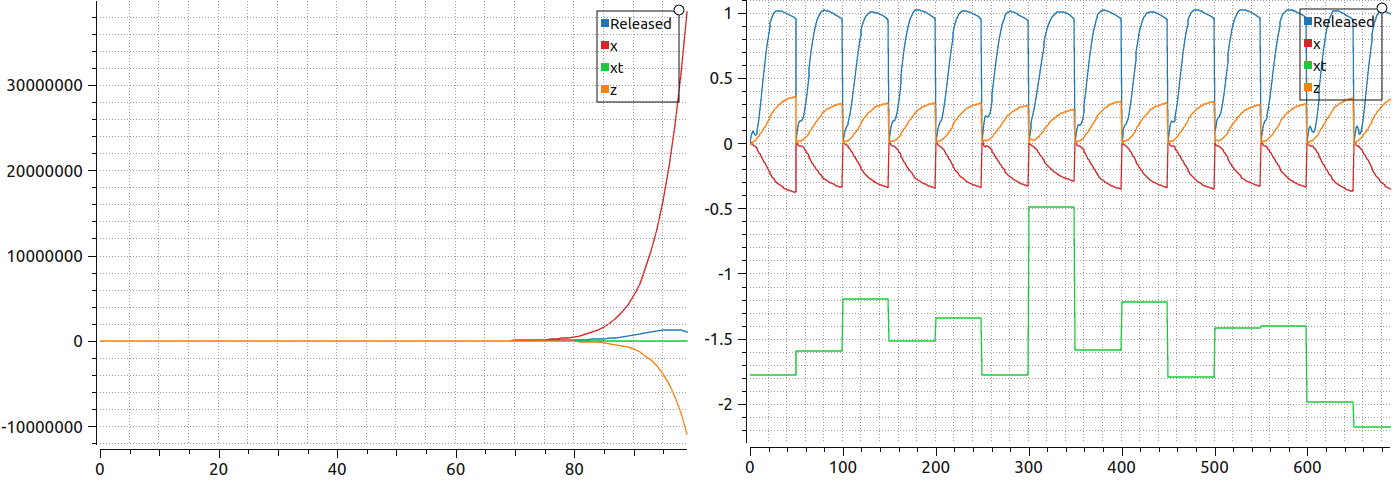
\includegraphics[height=5cm,page=1]{../img/qualitative_plots.png}
    \caption{Pa kreisi, trajektorija ierakstīta ar modeli, kam nepareizi definēta mērķa funkcija -- novedot pie autoregresora rezultātu diverģences. Pa labi, trajektorija, kuras kvalitatīvie aspekti liecina, ka parametru izvēle ir aptuveni pareiza. Abos gadījumos -- atlaišanas signāls, paredzētās x un z koordinātes, mērķa x koordinātes attiecībā pret laika soli.}
\end{figure}

\subsubsection{Validācija -- demonstrāciju un autoregresoru salīdzinājumi}

Taču kā jau minēts, ar subjektīviem vizuāliem spriedumiem vien nepietiek, lai būtu iespējams salīdzināt dažādu modeļu arhitektūru un hiperparametru kopu ietekmi uz rezultātiem. Kad pabeigta procesa sākotnējā atkļūdošana un iegūti modeļi, kas konverģē uz šķietami derīgiem rezultātiem, nākamais solis ir kvantitatīvu salīdzinājuma rādītāju ieguve. Problēma ar no gadījuma izlases ģenerētām trajektorijām ir objektīvu kvalitātes kritēriju trūkums. 

Ņemot vērā atdarinošās mašīnmācīšanās (un laikrindu ekstrapolācijas) problēmu pamatnostādnes, modeļa mērķis ir radīt tādas laikrindas konfigurāciju telpā, kas nav atšķi-ramas no tāda slēptā sadalījuma, kura izlase veido demonstrāciju kopu. Nekas nav zināms par pašu šo sadalījumu, un kaut kāda veida mākslīga tā izlases papildināšana ir ekvivalenta šīs pašas problēmas atrisinājumam. Taču pastāv divi teorētiski krasi atšķirīgi, bet praktiskā izpildījuma ziņā tuvi radniecīgi paņēmieni, ko var izmantot, lai izdarītu spriedumus par apmācības procesa spēju izpildīt pamatnostādni:

\begin{enumerate}
    \item novērtēt modeļa spēju aproksimēt pašu treniņu datu kopu. No teorētiskā viedokļa, jebkurš pietiekami liels un ``elastīgs'' modelis var pilnībā apgūt jebkuru tā apmācībā izmantoto datu kopu, taču praksē tas ne vienmēr izdodas. Var salīdzināt autoregresijas rezultātus ar treniņa kopas demonstrācijām pie tādiem pašiem sākuma parametriem;
    \item salīdzināt modeli ar izlasi no tā paša sadalījuma, kas veidojis apmācības datu kopu, bet kuras elementi tajā neietilpst. Jebšu, nošķirt pieejamos datus treniņa un validācijas kopās, no kurām tikai pirmā izmantota modeļa parametru iestatīšanai. Šādi tiek gūts priekšstats par iegūtā modeļa vispārināmību nezināmā sadalījuma ietvaros.
\end{enumerate}

Reālā izpildījuma ziņā abas metodes ir pilnīgi identiskas, atšķiras tikai datu kopa, kas tiek izmantota salīdzināšānai. To veic procedūras ar nosaukumu \textit{validation\_on\_test}, kas dažādajiem neironu tīklu izpildījumiem ir atšķirīgas, taču principā veic to pašu darbību secību. Tiek nolasīta izvēlētais datu korpuss -- apmācības vai validācijas. Tiek nošķirtas visas tā demonstrācijas, un katrai no tām tiek piekārtota atbilstoša tāda paša garuma autoregresora trajektorija un pievienota datu korpusa rindai

\begin{equation}
    (s_1, s_2, ..., s_n) \rightarrow \left ( (s_1, s_1), (s_2, s^{\theta}_2), ...,      (s_n, s^{\theta}_n) \right )
\end{equation}

Apvienotās trajektorijas atkal tiek savietotas vienā datu korpusā, un tas ar modeļa parametriem atbilstošu nosaukumu tiek saglabāts \textit{models/validation/} direktorijā. Visos apmācības skriptos tiek piemērota šī operācija gan ar apmācības, gan pārbaudes datu kopu. Kad pieejamas statistiski salīdzināmas laikrindas, iespējams aprēķināt dažādus skaitliskus novērtējumus to līdzībai -- par ko sīkāk diskutēts nākamajā nodaļā.

\subsubsection{Trajektoriju telpiska vizualizācija}

Ne divdimensionālas līknes, kas katra attēlo vienu konfigurācijas koor-dināti, ne dažādi abstrakti statistiski skaitliskie rezultāti nesniedz stabilu priekšstatu par to, vai iegūtais rezultāts telpā atgādina metienu, vai tas ietilpst robota kinemātisko ierobežojumu definētajā darba zonā, un vai tas radikāli nepārkāpj robota dinamiskās iespējas. Pirmkārt, šīs iekārtas ir jaudīgas un vērtīgas -- nepieciešams ar lielu piesardzību novērtēt jebkuru vadības sistēmu, pirms tiek pieļauta to radīto komandu izpilde uz fiziskas aparatūras. Otrkārt, pat, ja pieejama simulācijas vide, dažādu koordinātu sistēmu nesakritības, pār-traukuma punktu klātbūtne un citi faktori var nozīmēt, ka trajektoriju vai nu nav iespē-jams izpildīt -- plānošanas fāzē tiek pārkāpti kādi drošības nosacījumi -- vai arī grūti saprast, kas notiek, jo tiek veikti lieli lēcieni konfigurāciju telpā.

Tāpēc izstrādāta programma, kas spēj attēlot vienu vai daudzas pozīcijas un orientācijas vektoru laikrindas 3-dimensiju telpā. Kā svarīgākās prasības šim rīkam noteiktas sekojošās:

\begin{enumerate}
    \item jāspēj viennozīmigi noteikt katra laikrindas punkta telpiskā pozīcija un orientācija robota pamatnes koordinātu sistēmā;
    \item jābūt iespējai uzreiz vizualizēt daudzas trajektorijas ar tām piekārtotajām mērķa koordinātēm. Lietotājam jāspēj skaidri atšķirt blakus esošie metieni un to mērķi;
    \item jābūt iespējai savietot šīs vizualizācijas ar robota modeli, lai būtu iespējams tās izmantot dažādu nevēlamu nobīžu atkļūdošanā;
    \item jābūt uzskatāmam veidam kā noteikt, ka padots satvērējmehānisma atlaišanas sig-nāls.
\end{enumerate}

\begin{figure}[t!]
    \centering
    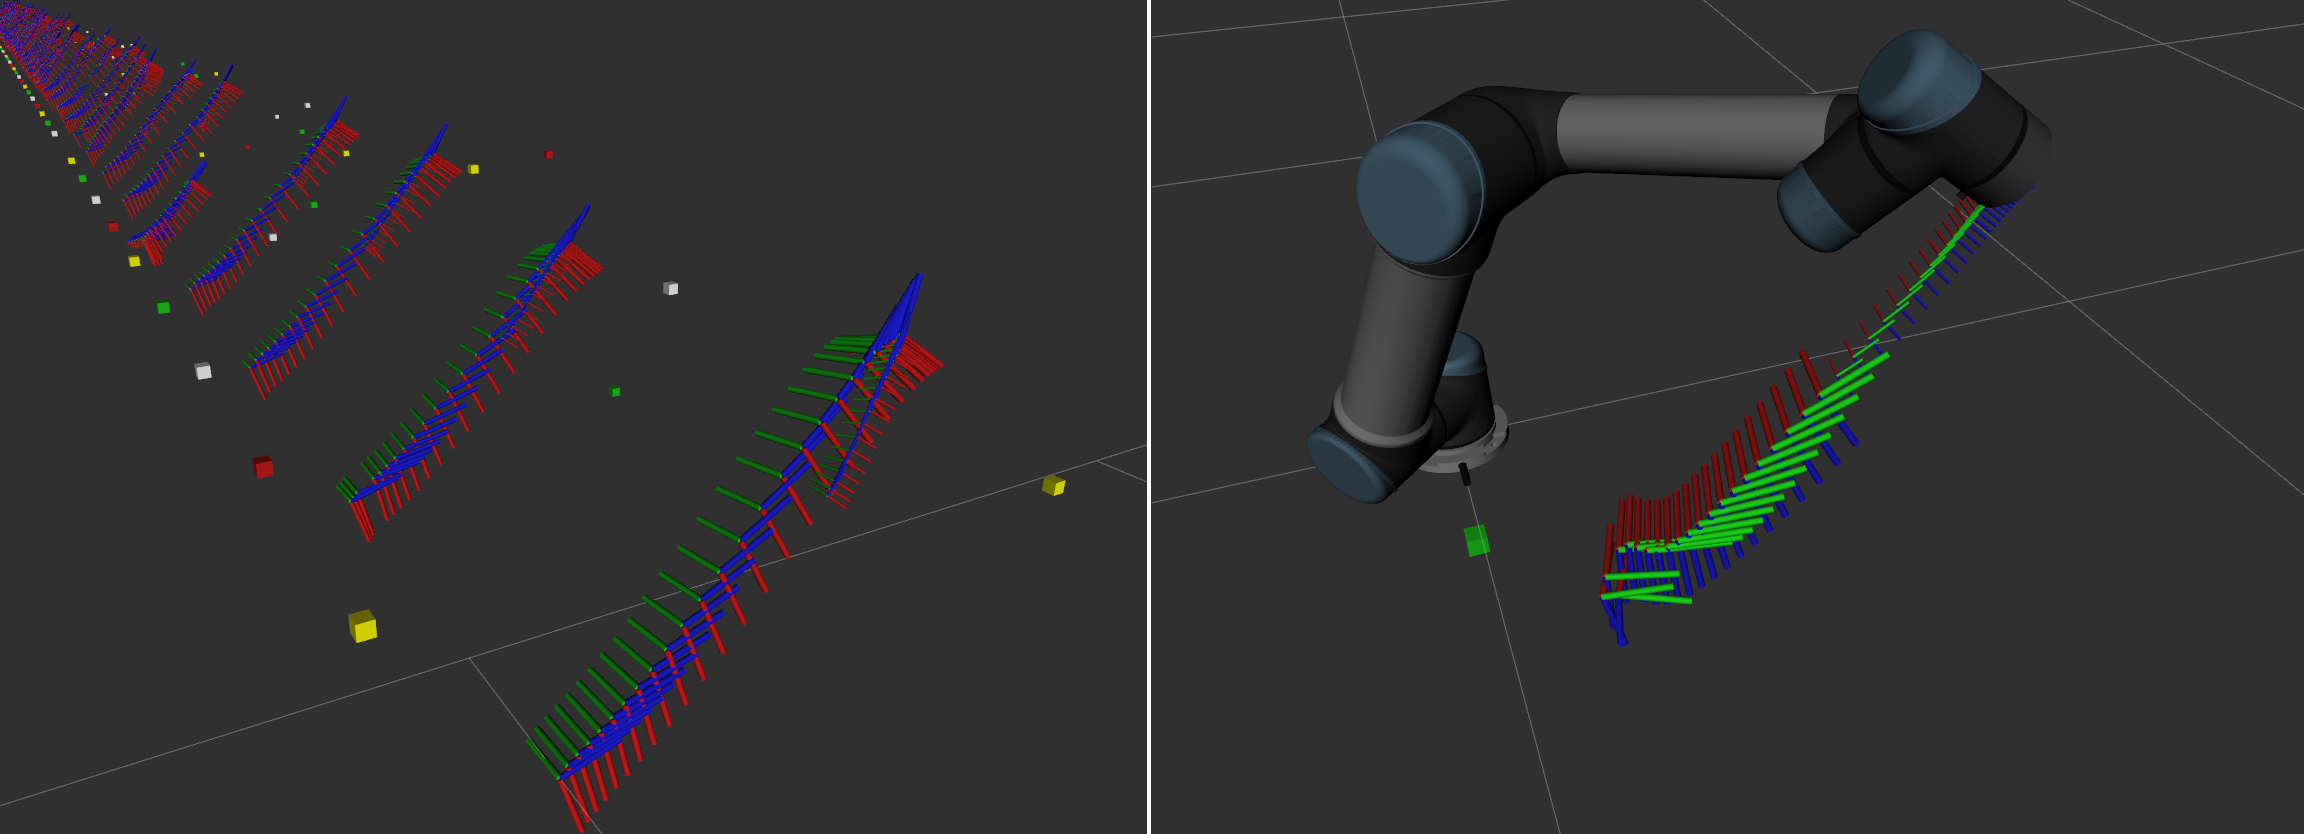
\includegraphics[width=16cm,page=1]{../img/trajectory_vis.png}
    \caption{Telpiski attēlotas autoregresora trajektorijas. Pa kreisi vizualizēts korpuss ar no gadījuma stāvokļiem ģenerētiem metieniem, pa labi -- trajektorija, kam piemēroti visi nepieciešamie pārveidojumi, lai tā sakristu ar robota efektora koordinātu sistēmu.}
\end{figure}

Šiem mērķiem ar Robotikas un mašīnuztveres personāla palīdzību izveidota ROS pakotne \textit{trajectory\_vis}, kas sastāv no viena valodā \textit{C++} rakstīta izpildfaila -- \textit{visualize.cpp}. Par grafisko attēlošanas vidi izvēlēts ROS platformā iekļautais rīks \textit{rviz}. Šajā rīkā iespējams attēlot patvaļīgi novietotus, patvaļīgas formas marķierus vai to masīvus. Šo marķieru iestatīšanai tiek izmantota tematu saskarne. Saskarni ar robota koordinātu sistēmām un marķieru modeļu zīmēšanu nodrošina bibliotēkas \textit{MoveItVisualTools} un \textit{Rviz-VisualTools}. 

Izsaucot lietojumprogrammu, tiek norādīti sekojošie argumenti:

\begin{enumerate}
    \item failsistēmas ceļš uz pareizi strukturētu \textit{.csv} failu, kas satur trajektorijas;
    \item attēlojamo trajektoriju skaits;
    \item pirmās trajektorijas sākuma indekss;
    \item pirmās trajektorijas beigu indekss.
\end{enumerate}

Programma nolasa datu korpusu un atrod tajā pozīcijas un orientācijas vektorus. Šie vektori tiek izmantoti, lai zīmētu koordinātu sistēmas marķierus -- simbolus, kas parāda, kā tiktu pārveidota pamata koordinātu sistēma, piemērojot tai attiecīgo pārvietojuma vektoru un rotācijas kvaternionu. Katru reizi, kad tiek sasniegts beigu indekss, pārvietojuma vektora $y$ ass tiek pārbīdīta un skaitīšana tiek atsākta -- tādējādi nodrošinot, ka daudzas trajektorijas var tikt attēlotas viena otrai blakus. 

To mērķa koordinātes apzīmē ar kuba formas marķieriem. Tā kā vizuāli ir grūti nošķirt, kurš beigu marķieris sakrīt ar kuru trajektoriju, ieviests vēl viens marķieris zem katra sākuma punkta. Katrai trajektorijai atbilstošie marķieri iezīmēti vienā krāsā, un secīgi tiek atkārtota virkne ar kontrastējošām krāsām. 

Papildus tiek nolasīts arī satvērējmehānisma konfigurācijas parametrs. To, vai satvērējmehānisms tiek uzskatīts par atvērtu, nosaka ar sliekšņa funkciju, kas piemērota tā skaitliskajai vērtībai. Vizuāli, tie punkti laikrindā, kad pudele teorētiski vēl būtu satverta, attēloti ar lielākiem marķieriem, bet tie, kuros tā jau ir atlaista -- ar samazinātiem.
 

\subsection{Trajektoriju izpilde uz robota}

No pētnieciskā viedokļa galvenā praktiskā darba daļa veltīta datu ieguves un modeļu apmācības uzdevumiem. Tā arī veido galveno zinātnisko pienesumu. Taču pēdējais un, iespējams, sarežģītākais uzdevums, kas veikts šī darba ietvaros, ir iegūto rezultātu izpilde uz fiziskas aparatūras. Tādi identificēti daudzi potenciālie šķēršļi iepriekš pētīto datizraces metožu pielietojumam ekspluatācijā un atrasts vismaz viens svarīgs virziens tālākai darbībai. Taču par spīti sastaptajiem sarežģījumiem izdevies realizēt paraug-demonstrāciju -- modeļa ģenerētu, uz reālas iekārtas izpildītu metiena kustību, kas veik-smīgi aizmet satvertu pudeli.

\subsubsection{Modeļa savietošana ar kontrolleri}

Kā jau sīkāk apspriests darba nodaļā par robotiem un to vadības problemātiku, ar pozīciju Dekarta koordinātu sistēmā vēl ne tuvu nepietiek, lai būtu iespējams izpildīt kādas robota darbības. Nepieciešams pārveidot telpisku pozīcijas informāciju robota asu dziņu vadības sistēmām saprotamos signālos, kas saistīti ar ātrumiem un paātrinājumiem locītavu konfigurācijas telpā. 

Atgriežoties pie izvēlētās modeļa arhitektūras un tā ģenerēto datu formāta, redzams, ka tie sastāda ar nemainīgu frekvenci atjaunotu pozīcijas un orientācijas mērķu virkni. Šāda tipa kontroles signāls sevī ietver visu nepieciešamo informāciju par vadāmo lielumu atvasinājumiem pēc laika, taču netiešā veidā. Darba gaitā aplūkoti augsta līmeņa paņē-mienu veidi, kā pārveidot šādu mērķu secību vadības signālos:

\begin{enumerate}
    \item kontrolleris -- pozas un orientācijas sekotājs, kas darbojas reālā laikā un potenciāli veido atgriezenisko saiti ar modeli;
    \item pilna kustības plāna aprēķināšana pirms izpildes;
\end{enumerate}

Uzskatāmākā priekšrocība kontrollera realizācijai ir iespēja izmantot modeli jau vairs ne kā tīru autoregresoru, bet ieviest atgriezenisko saiti caur fizikālo vai simulēto izpildes vidi. Kā ievadu nākamā stāvokļa mērķa iegūšanai varētu izmantot pozīcijas un orientācijas faktisko mērījumu, iespējams, mazinot sistemātiskas nobīdes starp modeļa inducēto stāvokļu kopu tīrā autoregresijā un reāli ieņemto konfigurāciju sadalījumu. Protams, jārēķinās arī ar iespēju, ka šādas sistemātiskas nobīdes pārāk daudz diverģē no inducētā sadalījuma, uz kura modelis ir apmācīts, un noved pie pasliktinātiem rezultātiem. Taču, ja paredzams kādreiz papildināt sistēmu ar stimulētās mācīšanās soli kā dažos literatūras analīzē aplūkotos pētījumos, atgriezeniskā saite ar vidi ir svarīga. Tāpat nav jāuztraucas par trajektoriju plānotāju piedāvātām laika parametrizācijas iespējām -- ja izdevies realizēt pozas sekotāju, ātruma informācija jau automātiski nokodēta vadības signālos.

Veikta šāda kontrollera prototipa izstrāde, izmantojot \textit{MoveIt\_servo} bibliotēku. Tā spēj pārvērst 6-dimensiju komandas, kas sastāv no telpiskā un leņķiskā ātruma vektoriem, robota locītavu vadību signālos bez lieliem lēcieniem konfigurāciju telpā, kamēr vien tas netiek novests tuvu singularitātēm vai kolīzijām. Taču sarežģījumu rada fakts, ka, lai pārvērstu stāvokļu virkni tās atvasinājumiem pielīdzināmos signālos, nepieciešams vēl viens kontrolleru slānis. Izmantojot atsevišķu PID kontrolleri katrai asij, kas ievadā saņem pozīcijas vai leņķa nobīdi novēlamās, to koeficientu atrašana kļūst par netriviālu uzdevumu. Tā kā vadības signāli atbilst pozīciju atvasinājumiem, nelielas nobīdes tajos var nozīmēt lielas kļūdas robota sasniegtajos novietojumos. Tomēr reāla laika kontrollera izmantošana varētu sniegt labākus rezultātus, strukturējot modeļus tā, lai tie paredz darbību -- telpisko ātrumu un paātrinājumu -- nevis stāvokļu laikrindu, kas būtu interesants virziens tālākiem pētījumiem.

Savukārt pilna trajektoriju plāna aprēķināšana ir metode, kuras izstrādes process saistīts ar mazākiem riskiem. Pastāv plašs atbalsts šādiem risinājumiem, un ROS kontekstā faktiski visas saskarnes ar robotu kontrolleriem balstītas uz pieņēmuma, ka uzdevums tiek realizēts kā diskrētu, iepriekš plānotu kustību virkne. Lai sagatavotu kustības plānu no punktu virknes Dekarta telpā, pietiek vien izsaukt augsti abstrahētu plānošanas komandu \textit{MoveIt} bibliotēkā. 

Galvenā problēma ar plānošanu ROS platformā ir tas, ka, kaut gan ļoti vienkārši precizēt konkrētiem laika punktiem piekārtotu locītavu konfigurāciju punktu iekļaušanu plānā un izpildi, nepastāv gatavi rīki, kas to pašu darītu ar telpiskiem punktiem. Tāpēc precīzi laikā parametrizēta telpiska plāna izpilde šobrīd nav iespējama -- nepieciešams izstrādāt rīku, kas spēj pārrēķināt plāna punktu laika vērtības, lai tās maksimāli tuvu atbilstu laikā parametrizētai telpisku punktu virknei. Tomēr, atšķirībā no kontrollera pieejas, kur nepieciešams pilnīgi strādājošs risinājums, lai kustības ģeometrija atbilstu vēlamajai, ar plānotāju iegūtās trajektorijas tai ir garantēti tuvas. Iespējams piemērot dažus vienkāršus uzlabojumus, lai plānu padarītu mazāk saraustītu un tā kopējo izpildes ilgumu pielīdzinātu prasītajam. Tad var novērtēt, vai modeļa ģenerētā trajektorija ie-kļaujas robota kinemātiskajos ierobežojumos, un pat izdarīt metienus ar samazinātu precizitāti.

\subsubsection{Robota trajektorijas plānošana un izpilde}


Tīri praktisku ierobežojumu dēļ trajektoriju plānošanas un izpildes programmatūru nācies radīt ar spēju darboties gan ar modeli, gan iepriekš ierakstītām laikrindām \textit{.csv} failos. Tas tāpēc, ka visa modeļu izstrāde šī projekta ietvaros ir veikta ar \textit{tensorflow} otro versiju, savukārt datori, kas tiek izmantoti fizisko robotu kontrolei, izmanto novecojušu ROS versiju -- kuras \textit{Python} versija nav savietojama ar jauno \textit{tensorflow}. Tāpēc sākotnēji simulācijas videi sagatavotais skripts \textit{setpoint\_from\_trajectory.py}, kas pieejams \textit{testpackage/scripts} direktorijā, papildināts ar iespēju nolasīt iepriekš sagatavotus failus un pārveidots saderībai ar \textit{Python 2.7}.

Vadības programmas pamatā ir \textit{MoveIt} bibliotēkas piedāvātā saskarne. Atkarībā no datu avota iespējams vai nu ielādēt iepriekš apmācītu modeli un noģenerēt autoregresora trajektoriju, vai arī tiešā veidā šādu trajektoriju iegūt no faila. Svarīgi, ka atkarībā no izvēlētā robota un kustību uztveres procesā izmantoto cieto ķermeņu konfigurācijas, iespējamas atšķirības starp to izmantotajām koordinātu sistēmām. Tāpēc nepieciešams veikt orientācijas pārveidojumus un novietojuma pārbīdi.

Tiek atrasti orientācijas nobīdes versori

\begin{equation}
    q_{offset} = q_r^{-1}q^{\pi}_{base}
\end{equation}
\begin{equation}
    q_{restore} = q_{offset}^{-1}
\end{equation}

$q^{\pi}_0$ apzīmē sākuma rotāciju -- kvaternionu, kura apzīmētā efektora simulatora orientācija ir ekvivalenta robota neitrālai robota sākuma orientācijai, ko apzīmē ar $q_r$. $q_{offset}$ tad ir nobīde starp šīm orientācijām, ņemot vērā arī atšķirīgo koordinātu sistēmu. Modeļa izmantošanai nepieciešams pārnest robota sākuma stāvokli uz tā apmācības kopā pielīdzināmu efektora stāvokli

\begin{equation}
    s^{\pi}_0 = (r^{\pi}_0, q^{\pi}_0 , g_0)
\end{equation}
\begin{equation}
    r_0 = x_0, y_0, z_0 = 0 = r^r_0 - r^r_0
\end{equation}
\begin{equation}
    q^{\pi}_0 = q^{r}_0q_{offset}
\end{equation}
\begin{equation}
    g_0 = 
    \begin{cases}
        1, \text{ ja atvērts} \\
        0
    \end{cases}
\end{equation}
, kur $r^r, r^{\pi}$ apzīmē robota, modeļa pozīciju, $q^{\pi}, q^r$ apzīmē to orientācijas, bet $g_0$ -- sākotnējo satvērējmehānisma stāvokli. Iegūto laikrindu pēc tam pārveido atpakaļ uz robota koordinātu sistēmu 

\begin{equation}
    s^{r}_t = (r^r_t, q^r_t , g_t)
\end{equation}
\begin{equation}
    r^r_t = r^{\pi}_t + r^r_0
\end{equation}
\begin{equation}
    q^r_t = q^{\pi}_tq_{restore}
\end{equation}

Satvērējmehānisma vadības signālam tiek piemērota sliekšņa funkcija ar histerēzi

\begin{equation}
    g^r_t = 
    \begin{cases}
        0, \text{ ja } \forall u < t, g^{\pi}_u < \delta \\
        1
    \end{cases}
\end{equation}

Faktiski vienīgais pārveidojums, kas jāveic tiešajā virzienā (no robota uz modeļa sistēmu) ir sākuma orientācija, ja tā atšķiras no neitrālas efektora orientācijas. Strā-dājot ar ierakstītu trajektoriju, notiek tikai inversie pārveidojumi (no modeļa uz robota sistēmu).

Lai varētu punktus izmantot trajektorijas plāna ieguvē, nepieciešams no tiem izveidot ROS komunikācijas modeļa robota pozas (pozīcijas un orientācijas) apraksta ziņojuma struktūras \textit{trajectory\_msgs.msg.Pose}. No šādu objektu masīva var iegūt kustības plānu ar \textit{move\_group.compute\_cartesian\_path} metodi, taču šādam plānam ir patvaļīga laika para-metrizācija. Lai to tuvinātu reālai demonstrācijai, vispirms tiek veikta laika repara-metrizācija, kas minimizē telpiskos un leņķiskos paātrinājumus, izmantojot \textit{``Time-Opti-mal Trajectory Generation''} algoritmu \cite{kunz2012time}. Pēc tam visi laika intervāli tiek proporcionāli pārveidoti, lai kopējais plāna ilgums sakristu ar trajektorijā paredzēto.

\subsubsection{Asinhrona satvērējmehānisma vadība, ātrdarbība}

Vienkāršākais veids, kā realizēt kustības plāna izpildi, būtu izmantot to pašu \textit{mo-ve\_group} saskarni, kas piedāvā \textit{execute} metodi. Tai kā argumentu nepieciešams padot trajektoriju locītavu konfigurācijas telpā, un, iestatot argumentu \textit{wait} uz nepatiesu vērtību, šis izsaukums nav bloķējošs. Taču jāatceras, ka \textit{move\_group} īstenībā sastāv no klienta abstrakcijām \textit{MoveGroup} darbības serverim ROS vidē. Kā jau minēts ROS platformā pieejamo saziņas mehānismu pārskatā, komunikācija ar šāda tipa serveriem seko galīgā automāta modelim, un visas šādas augsta līmeņa komandas bloķē izsaukumus uz serveri, pat ja izsaucēja kodā tās ļauj turpināt izpildi, negaidot atbildi ar darbības pieprasījuma rezultātu. Tas nozīmē, ka, pat ja serveris tiktu konfigurēts kontrolēt gan robotu, gan tā darbarīku, nebūtu iespējams ar tā palīdzību veikt pudeles atlaišanu, kamēr robots vēl ir kustībā.

Tāpēc nepieciešams izmantot paralēlus un neatkarīgus ziņapmaiņas kanālus, lai nodotu atlaišanas komandu pareizajā kustības izpildes brīdī. Vienkāršākais variants, kā to varētu mēģināt realizēt, ir noteikt laiku kopš darbības sākuma, kad jāatlaiž pudele, un ar laika aizturi padot komandu. Taču tas būtu ārkārtīgi neprecīzi bez stingrām reālā laika garantijām un ar vērā ņemamu aizturi starp kustības pieprasījuma nodošanu un reālās kustības sākumu robota kontrollerī.

Tāpēc nolemts tiešā veidā izmantot robota locītavu kontrollera piedāvāto darbības serveri -- apejot \textit{MoveGroup} -- un izmantot pēc robota reālās pozīcijas parametrizētu atzvanīšanas funkciju, lai nodotu satvērēja atlaišanas signālu. Tā tiek izsaukta katru reizi, kad darbības serveris publicē atgriezeniskās saites ziņu. Principā iespējams izsaukuma ietvaros iegūt robota telpisko pozu, taču tas nozīmē, ka jāveic papildu saziņa ziņampaiņas sistēmā -- ar papildu aizturēm. Tā kā izpildāmās trajektorijas ir ātras -- vēlamā atlaišanas signāla izpildes precizitāte ir ne zemāka kā 0,05 sekundes -- nolemts jau iepriekš noteikt vēlamo locītavu konfigurāciju un salīdzināt robota pašreizējo stāvokli ar to. Šī vēlamā konfigurācija tiek noteikta, aprēķinot kustības plānu telpiskajai trajektorijai līdz atlaišanas punktam un ņemot pēdējo. Visas darbības, kas veicamas ar locītavu stāvokļa kontrollera darbību servera palī-dzību, apkopotas klasē \textit{``FollowTrajectoryWrapper''}, jo nepieciešama iespēja nodot dinamiskus papildu argumentus atzvanīšanas funkcijai. 

\begin{figure}[t!]
    \centering
    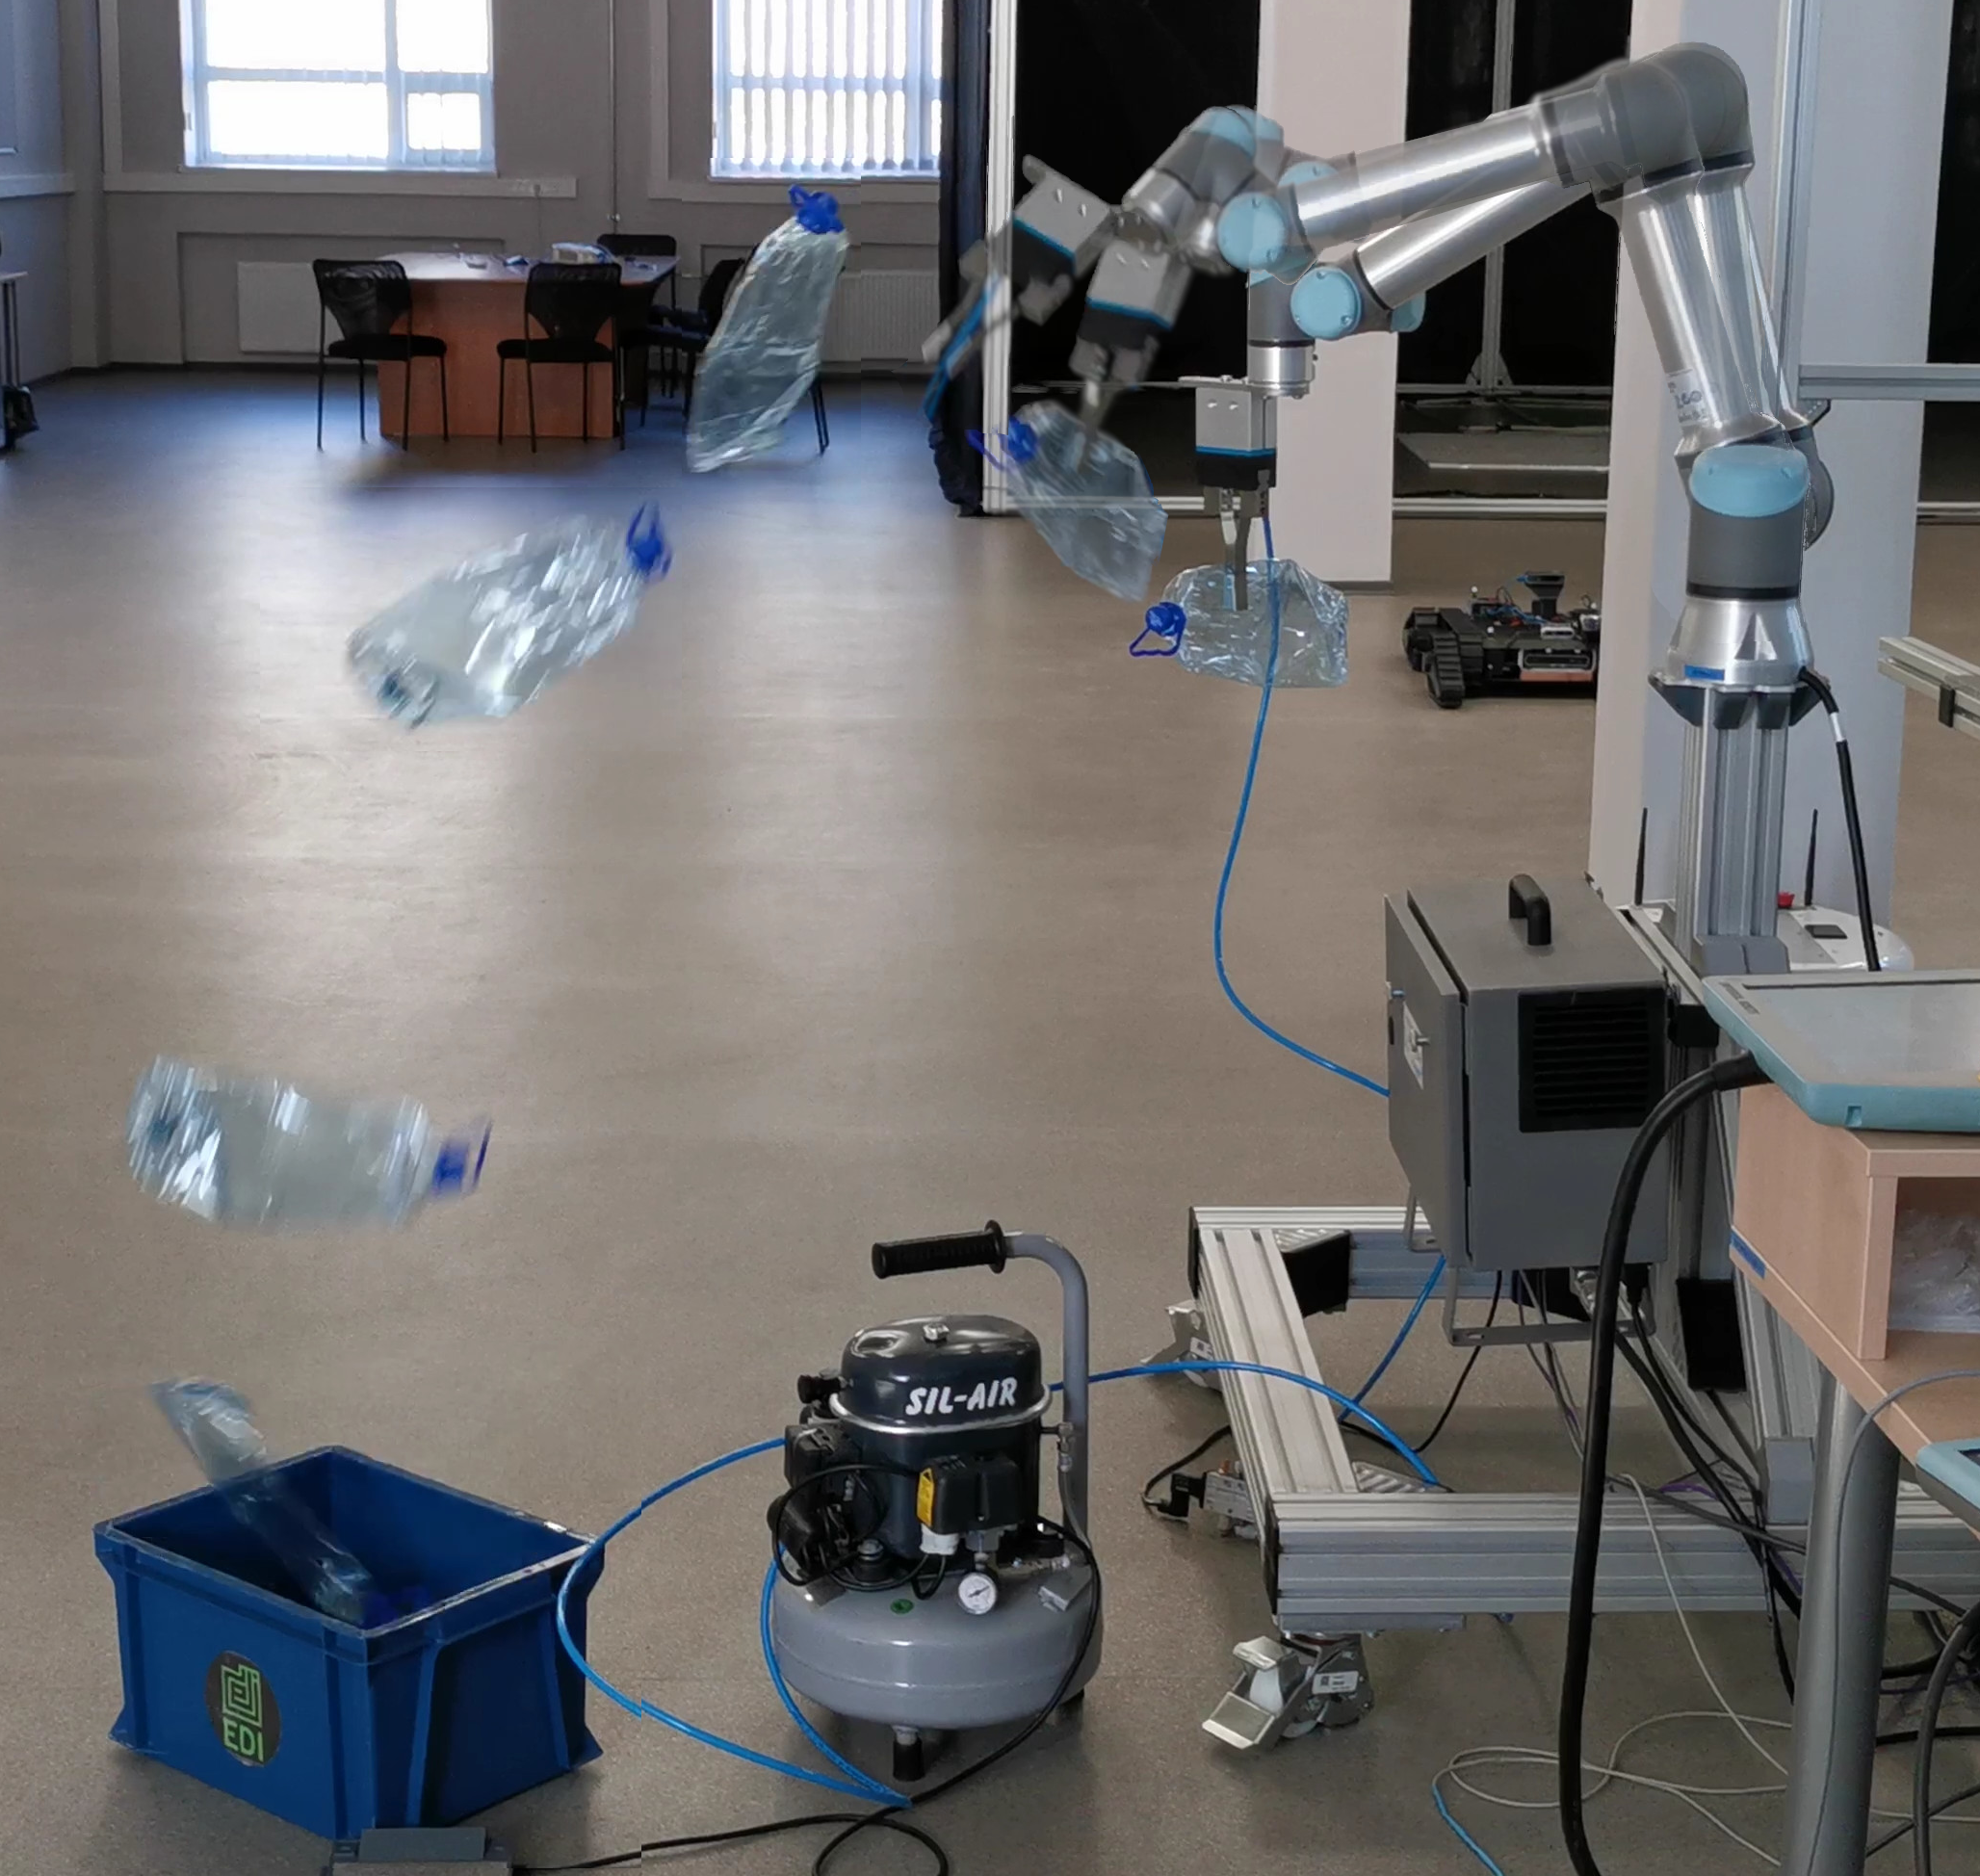
\includegraphics[height=7.4cm,page=1]{../img/action_sequence.png}
    \caption{Paraugdemonstrācija -- klasiskā neironu tīkla ģenerēta trajektorija.}
\end{figure}


Tā kā citu pētījumu ietvaros izvēlētais robots parasti ir aprīkots ar \textit{``Robotiq 2f''} efektoru, kas piedziņai izmanto elektromotorus, saziņu realizē pār \textit{EtherCAT} protokolu un arī kontrolējams ar darbības servera palīdzību, tam izveidota klienta klase \textit{GripperActionWrapper}. Simulācijas vidē šis ir pietiekams risinājums, un ar to izdodas veikt trajektoriju izpildi.

Taču mēģinot veikt paraugdemonstrāciju ar fizisko robotu konstatēts, ka elektromotoru piedziņa nav pietiekami ātrdarbīga, lai paredzami un īstajā trajektorijas punktā veiktu elastīga metamā objekta atlaišanu -- pat iestatot maksimālu darbības ātrumu. Var, protams, ieviest manuālas korekcijas programmas kodā -- mākslīgi pārbīdīt atlaišanas punktu, to pielāgojot katras trajektorijas formai, vai ieregulējot satveršanas ciešumu tā, lai tas ļoti precīzi atbilstu konkrētajai pudelei un tās pašreizējam tvērienam. Taču tādā gadījumā vairs netiek objektīvi vērtēta modeļa spēja pareizā laika un telpas punktā padot atlaišanas signālu. Lai risinātu šo problēmu, robots aprīkots ar daudz ātrāku pneimatisko satvērējmehānismu. Tā darbībai pietiek ar robota kontrollera digitālā izvada pieslēgšanu 5/2 solenoīdvārstam. \textit{Ur5e} robota kontrolleris nepiedāvā darbības serveri digitālo izvadu vadībai, tāpēc jāizmanto trešā no ROS pieejamajām saziņas metodēm -- pakalpojuma serveris. Komunikāciju ar \textit{set\_io} pakalpojumu realizē klase \textit{GripperServiceWrapper}.




%
%
%
%
%
%
%
%
%
%
% CHAPTER 5
% CHAPTER 5
% CHAPTER 5
% CHAPTER 5
% CHAPTER 5
% CHAPTER 5
% CHAPTER 5
% CHAPTER 5
% CHAPTER 5
% CHAPTER 5
% CHAPTER 5
% CHAPTER 5
% CHAPTER 5
%
%
%
%
%
%
%
%
%

\newpage
\section{Rezultāti}

Paraugdemonstrācijas uz robota atstāj iespaidu uz skatītājiem no malas un pa-līdz popularizēt gūtos rezultātus, taču tās nav darba pašmērķis, un pilnīgi noteikti nav pietiekamas, lai izdarītu objektīvus spriedumus par dažādus datu ieguves un modeļu apmācības procesa aspektu priekšrocībām un trūkumiem. Nepieciešams atrast piemērotus skaitliskus novērtējumus, kas ļauj pēc iespējas vienlīdzīgāk salīdzināt dažādus risinājumus.

\subsection{Novērtējumi, to aprēķins}

Iepriekšējā nodaļā aprakstīts, kā tiek iegūti trajektoriju paraugi validācijai -- ap-mācības un pārbaudes datu kopu demonstrācijas ar tām piekārtotām modeļu ģenerētām trajektorijām pie tādiem pašiem sākuma nosacījumiem. Lai aprēķinātu novērtējuma mērus un apkopotu tos vienā datu korpusā, izvedots skripts \textit{generate\_evaluation\_me-trics.py}, kas atrodams projekta repozitorijā, \textit{models/} direktorijā.

Tā kā pie katra ar dažādiem parametriem apmācīta modeļa iegūtas divi validācijas datu faili -- treniņa un testa -- to skaits ir pārāk liels, lai būtu praktiski veikt aprēķinu katram atsevišķi, iestatot nepieciešamos parametrus manuāli. Tāpēc uzrakstītais kods iegūst katru modeli aprakstošo informāciju no saglabātā faila nosaukuma. Tie ir lielumi kā modeļa paveids, parametru skaits, apmācībā izmantotā datu kopa -- neilgi pirms darba noslēguma ievākta jauna demonstrācijas datu kopa, kas labāk atbilst robota kine-mātiskajiem ierobežojumiem un ļauj praktiski izpildīt trajektorijas, neuztraucoties par pozām ārpus tiem -- apmācības epohu skaits, laika signāla esamība vai neesamība (agrīni modeļi apmācīti bez tā). Šī informācija var tikt izmantota, lai grupētu un filtrētu rezultātu tabulas rindas analīzes mērķiem.

Lai varētu veikt dažādo novērtējumu aprēķinus, pats datu fails tiek nolasīts, izmantojot \textit{pandas} datu korpusu apstrādes bibliotēku, un dažādās skaitliskās vērtības tiek aprēķinātas pamatā ar tenzoru operācijām \textit{numpy} skaitļošanas bibliotēkā.

\subsubsection{Datu kopu tuvības mēri}

Pirmā skaitlisko novērtējumu kategorija, ko var aprēķināt, lai salīdzinātu jebkādus datus, ir datu kopu tuvības mēri, kas aizgūti no statistikas -- Pīrsona korelācijas koeficients, dažādu pakāpju distances metrikas, kosinusu līdzība. Problēma ar šādu metožu izmantošanu ir fakts, ka tās visas ir operācijas, kurām argumentā nepieciešams padot divus vektorus -- vienā rindā sakārtotas skaitļu virknes. Efektora konfigurāciju laikrindas sastāv no vektora katrā laika solī -- tātad tās ir matricas no lineārās algebras viedokļa. Šeit pielietotais risinājums ir gaužām vienkāršs -- datu kopas sašķeltas demonstrācijas un ģenerētajās matricās. Katra no tām tiek ``saplacināta'':

\begin{equation}
    \begin{bmatrix}
        x_{11} & \ldots & x_{1m} \\
        \vdots & \ddots & \vdots \\
        x_{n1} & \ldots & x_{nm}
    \end{bmatrix}
    \rightarrow
    (x_{11}, ..., x_{n1}, x_{12}, ..., x_{nm})
\end{equation}

Tad tām var aprēķināt vektoru līdzības novērtējumus. Pirmais ir statistikā ļoti plaši izmantotais Pīrsona korelācijas koeficients $r_{xy}$, kam var atrast vienkāršu vektoriālu izteiksmi, kura izmanto centrētus vektorus $x^c, y^c$ \cite{pearson_vector}. 

\begin{equation}
    \overline{x} = \frac{1}{nm} \sum_{i=1}^{nm} x_i
\end{equation}
\begin{equation}
    x^c = (x_i - \overline{x}, x_2 - \overline{x}, ..., x_{nm} - \overline{x})
\end{equation}
\begin{equation}
    r_{xy} = \frac{x^c \cdot y^c}{\Vert x^c \Vert \Vert y^c \Vert}
\end{equation}

Ļoti līdzīga izteiksme ir kosinusu līdzībai, kas ir vienāda ar $1$ paralēliem vektoriem, $0$ -- ortogonāliem, bet pretējiem ir $-1$ \cite{cosine_sim}. Aplūkojot formulu uzreiz arī kļūst skaidrs, ka Pīrsona korelācijas koeficienta ģeometriskā interpretācija ir šī pati kosinusu līdzība, tikai centrētiem vektoriem.

\begin{equation}
    d_{cos}(x,y) = \frac{x \cdot y}{\Vert x \Vert \Vert y \Vert}
\end{equation}

Eiklīda un Manhetenas distance pieder pie distances metrikām -- funkcijām kas ir simetriskas un kam izpildās trīsstūra nevienādība \cite{metrics}.

\begin{equation}
    d_{euclidean}(x,y) = \Vert x - y \Vert
\end{equation}
\begin{equation}
    d_{manhattan}(x,y) = \Vert x - y \Vert_1 = \sum_{i=1}^{nm} \vert x_i - y_i \vert
\end{equation}

Kā redzams, pirmā atbilst telpiskajam attāluma jēdzienam, savukārt otrā vienkārši pilnīgi neatkarīgi novērtē atšķirību katrā vektora dimensijā, tad saskaita visas.

\subsubsection{Vidējās novirzes laika soļa ietvaros}

Iespējams mērīt ne tikai tuvību starp datu kopām kopumā, bet novērtēt to vidējās, maksimālās, minimālās, u.c. nobīdes katra laikrindas soļa ietvaros. Tiek aprēķinātas vidējās Eiklīda un Manhetenas distances, kur tiek uzreiz novērtēti konfigurāciju vektori $x_t, y_t$

\begin{equation}
    \overline{d_{euclidean}}(x,y) = \frac{1}{n} \sum_{t=1}^{n} \Vert x_t - y_t \Vert
\end{equation}
\begin{equation}
    \overline{d_{manhattan}}(x,y) = \frac{1}{n} \sum_{t=1}^{n} \Vert x_t - y_t \Vert_1
\end{equation}

Eiklīda distanci var aprēķināt arī konkrēti pozīcijas kļūdai.

\begin{equation}
    \overline{\Delta r}(x,y) = \frac{1}{n} \sum_{t=1}^{n} \Vert r^x_t - r^y_t \Vert
\end{equation}

Savukārt orientācijas kļūdai var aprēķināt leņķisko nobīdi starp kvaternioniem \cite{quat_distance}.

\begin{equation}
    \overline{\alpha}(x,y) = \frac{1}{n} \sum_{t=1}^{n} \arccos \left (2(q^x_t \cdot q^y_t)^2 - 1 \right )
\end{equation}

Primitīvs atlaišanas signāla kvalitātes novērtējums būtu kategorisks salīdzinājums (vienāds ar 0, ja signāli laika solī sakrīt, bet 1, ja nesakrīt):

\begin{equation}
    g'_t = 
    \begin{cases}
        1, \text{ ja } g_t > 0,5 \\
        0
    \end{cases}
\end{equation}
\begin{equation}
    \overline{\Delta g}(x,y) = \frac{1}{n} \sum_{t=1}^{n} \vert g^x_t - g^y_t \vert
\end{equation}

\subsubsection{Metiena parametru aplēšana}

Augstāk uzskaitītie vispārīgi pielietojamie rādītāji var būt noderīgi dažādu modeļu apmācības aspektu vērtēšanai, taču, tā kā sasniedzamais rezultāts ir metiena realizācija, iespējams sastādīt daudz specifiskākus modeļa novērtējumu. Pirmās kārtas aproksimācijai var pieņemt, ka metienu pilnībā definē tā palaišanas punkts un ātruma vektors. Lai salīdzinātu ātrumu vektorus, ar kosinusu līdzību vien nepietiek -- svarīga ir arī vektoru norma. Vispirms, atceramies, ka katrs validācijas datu korpuss sastāv no demonstrāciju un ģenerētu trajektoriju pāriem

\begin{equation}
    \mathcal{D}_{val} = \left (  (\tau_{d1}, \tau_{g1}), ...
     (\tau_{dk}, \tau_{gk}) \right )
\end{equation}

Tāpēc sastādīts sekojošais vienādojums

\begin{equation}
    v_t = r_t - r_{t-1}
\end{equation}
\begin{equation}
    \overline{\epsilon_v}(\mathcal{D}_{val}) = \frac{1}{k} \sum_{\mathcal{D}_{val}}
    \vert \Vert v^d_{trd} \Vert - v^d_{trd} \cdot v^g_{trg} \vert 
\end{equation}
, kur $t_{rd}, t_{rg}$ ir attiecīgi $\tau_{d}, \tau_{g}$ atlaišanas signāla paceļošās frontes laika soļi, bet $v_t$ apzīmē aptuvenos ātrumus (pār-vietojumu diferences). Lai šādam novērtējumam būtu jebkāda nozīme, gadījumos, kad kādā no ģenerētajām trajektorijām $\tau_{g}$ atlaišanas signāls nav padots, tas pieņem nedefinētu vērtību.

\begin{equation}
    \nexists s_t \in \tau_{g}, g(s_t) = 1 
    \Rightarrow
    \overline{\epsilon_v}(\tau_{d},\tau_{g}) \equiv +\infty 
\end{equation}

Līdzīgi var novērtēt arī kļūdu palaišanas momenta pārvietojumos.

\begin{equation}
    \overline{\epsilon_r}(\mathcal{D}_{val}) = \frac{1}{k} \sum_{\mathcal{D}_{val}}
    \Vert r^d_{trd} - r^g_{trg} \Vert 
\end{equation}

Pacilājot jautājumu par to, kā abas šīs vērtības varētu apvienot vienā novērtējumā, secināts, ka tik tālu izdarīto var novest līdz galam un aplēst novirzi starp abu palaišanas ātruma un pozīcijas vektoru pāru definēto brīvā kritiena parabolu krustpunktiem ar mērķa koordinātu horizontālo plakni. Īsāk, ģeometriski ``simulēt'' metienu un novērtēt, cik tālu no demonstrācijas modelis ir trāpījis. No pamatskolas matemātikas zināms, ka brīvo kritienu var aprakstīt ar vienādojumiem

\begin{equation}
    x(t) = x_0 + v_xt 
\end{equation}
\begin{equation}
    y(t) = y_0 + v_yt 
\end{equation}
\begin{equation}
    z(t) = z_0 + v_{z0}t - \frac{g}{2}t^2 
\end{equation}
, kur $q \approx 9,81 \frac{m}{s^2}$ ir tipiska gravitācijas paātrinājuma vērtība uz zemes virsmas. Tad lai atrastu $x,y$ koordinātes parabolas krustpunktam ar plakni, vispirms tiek atrasta pozitīvā sakne $t_{intersect}$ sekojošam vienādojumam

\begin{equation}
    z_0 - z_{target} + v_{z0}t_{intersect} - \frac{g}{2}t_{intersect}^2 = 0
\end{equation}

un ievietota horizontālo koordinātu vienādojumos

\begin{equation}
    r_{intersect} = \left ( x(t_{intersect}), y(t_{intersect}), z_{target} \right )
\end{equation}

Vidējo metiena kļūdu tad var novērtēt kā

\begin{equation}
    \overline{\epsilon_{throw}}(\mathcal{D}_{val}) = \frac{1}{k} \sum_{\mathcal{D}_{val}}
    \Vert r^d_{intersect} - r^g_{intersect} \Vert 
\end{equation}


\subsubsection{Grafiku ģenerēšana un saturs}

\begin{figure}[t!]
    \centering
    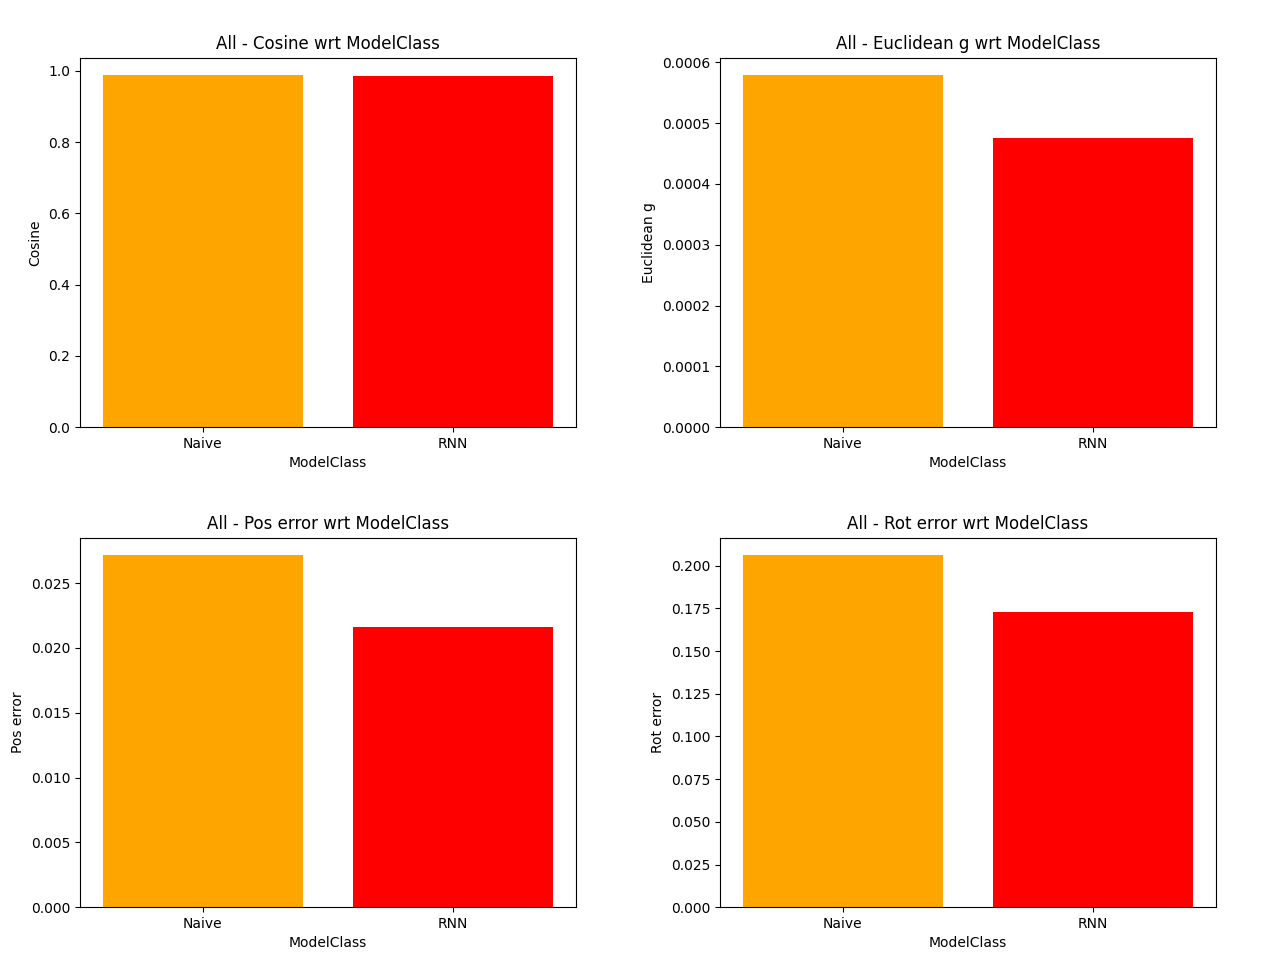
\includegraphics[width=16cm,page=1]{../img/rnn-naive-global-stepwise.png}
    \caption{Datu korpusu vispārīgās tuvības rādītāji (kosinusu līdzība, Eiklīda distance) un vidējās telpiskās/rotācijas novirzes laika soļa ietvaros -- RNN un klasiskajam neironu tīklam.}
\end{figure}

Visas šajā nodaļā izmantotās diagrammas ir ģenerētas programmatiski divos soļos. Vispirms no iepriekš aprēķinātā metriku datu korpusa tiek izdalītas katras sakarības attēlošanai nepieciešamo datu kopas, kas pēc tam tiek izmantotas grafikus saturošu attēlu ģenerēšanai. Par šiem uzdevumiem atbild darba repozitorija \cite{md_repo} \textit{models/} direktorijā atrodamie skripti \textit{comparison\_table\_generator.py} un \textit{draw\_plots.py}.

Situācijās, kad tiek salīdzinātas dažādas modeļu klases vai veikti vispārīgi modeļu veiktspējas novērtējumi pie dažādiem hiperparametriem, uzskatāmības labad tiek atrastas novērtējumu maksimālās (vai minimālās, atkarībā no novērtējuma būtības) vērtības pie katra, bez fiksēto hiperparametru kopas. Tas nesniedz tik detalizētu ieskatu apmācības procesa atkarībās no katra argumenta, bet ļauj globāli novērtēt, ar kuru modeli sasniegti labāki rezultāti, vai lielāki modeļi sasniedz labākus rezultātus, u.t.t. 

\begin{figure}[t!]
    \centering
    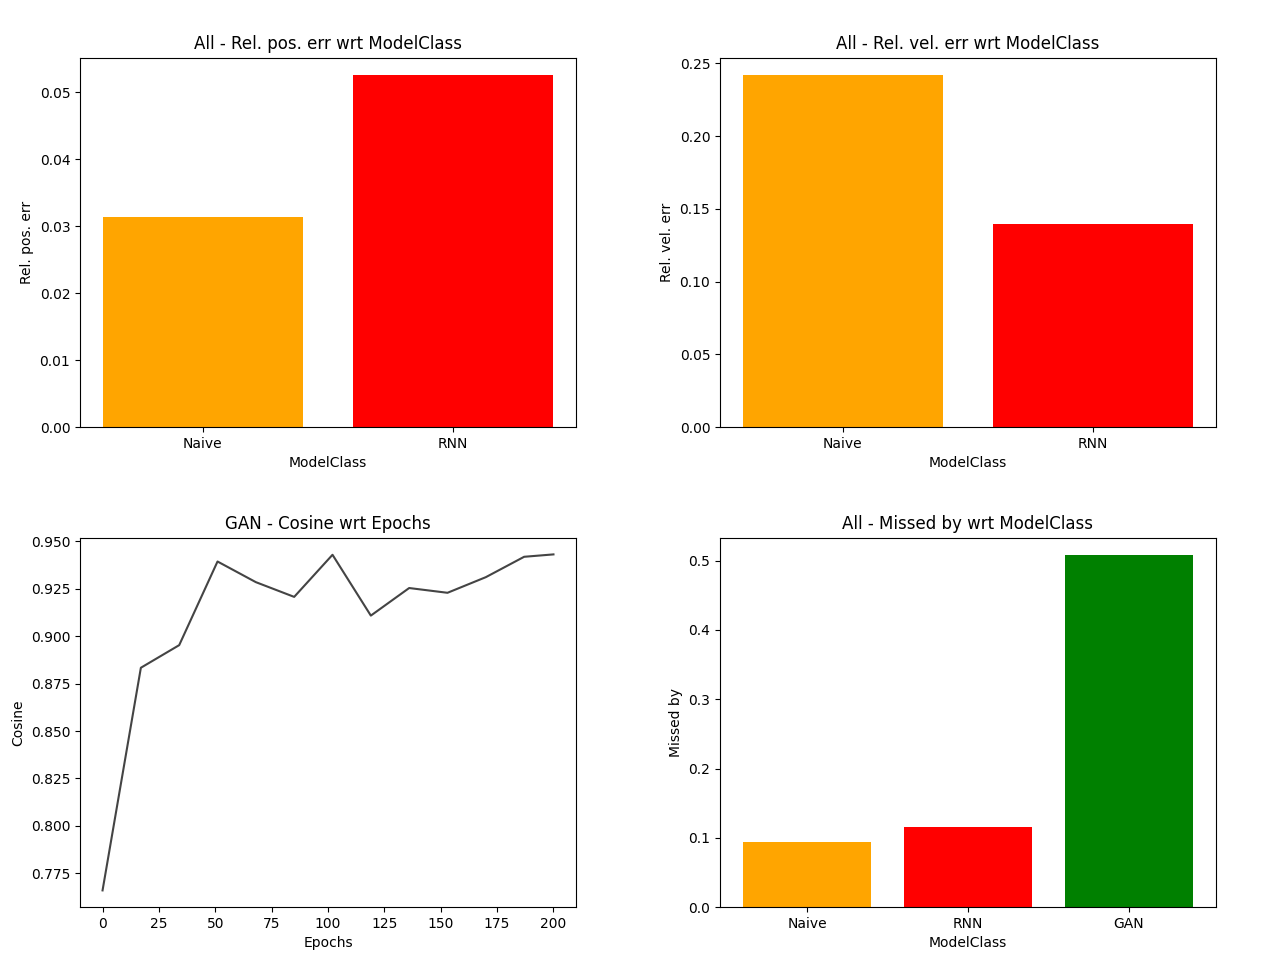
\includegraphics[width=16cm,page=1]{../img/throw_metrics_gan.png}
    \caption{Augšējā rindā -- labākās sasniegtās vidējā atlaišanas punkta novietojuma un ātruma vektora noviržu vērtības. Apakšā pa kreisi -- pietiek ar jau rudimentāru GAN arhitektūru, lai vispār notiktu modeļa konverģence. Tomēr no RNN un klasiskā neironu tīkla sasniegtajiem rezultātiem tā tomēr atpaliek.}
\end{figure}

Papildus veikta arī detalizēta novērtējumu attēlošana atkarībā no konkrētiem lielumiem, turot pārējos konstantus -- taču lielais apmācīto modeļu skaits nozīmē, ka grūti šādus datus attēlot uzskatāmi. Tāpēc ieviests kompromiss -- situācijās, kad apskatītas līknes ar daudzām fiksēto argumentu kopām, izvēlētas pa divām ``labākajām'' -- pie lielākās apmācības kopas (atceroties, ka tas ir novērtējums modeļa spējai aproksimēt tā apmācības datus) un mazākās validācijas kopas (kas sniedz ieskatu slēptā datus ģenerējošā sadalījuma apguvē, taču mazāko izmēru dēļ noved pie neskaidrākiem rezultātiem un sakarībām).

\subsection{Sasniegtie rezultāti dažādām modeļu klasēm}


Pirmais, ko var darīt, kad iegūti šādi sistemātiski aprēķināti kvalitātes mēri, ir salīdzināt ar dažādām modeļu arhitektūrām sasniegtos labākos rezultātus. 11. attēlā redzamas diagrammas, kurās salīdzināti labākie globālie $\tau_d, \tau_g$ tuvības mēri un novirzes katrā laika solī iegūtajās konfigurācijās. Kā redzams, kosinusu līdzība ir ļoti augsta abiem modeļiem, liecinot, ka datu kopa tik tiešām tiek apgūta. Metrikas bieži vien labākas ir rekurentiem modeļiem, tas pats attiecas arī uz vidējām nobīdēm. 

Var ar pārliecību apgalvot, ka rekurentais neironu tīkls mazāk diverģē no treniņa kopā novērotajiem metieniem, taču šī atšķirība nav radikāla. Izsakot grafiku mērogu cilvēkam saprotamās mērvienībās, rekurentais tīkls uzlabo vidējo pozīcijas kļūdu no 2,5 uz 2cm, bet vidējo orientācijas vektora leņķisko nobīdi -- no 11,5 uz 9,8 grādiem.

\begin{figure}[t!]
    \centering
    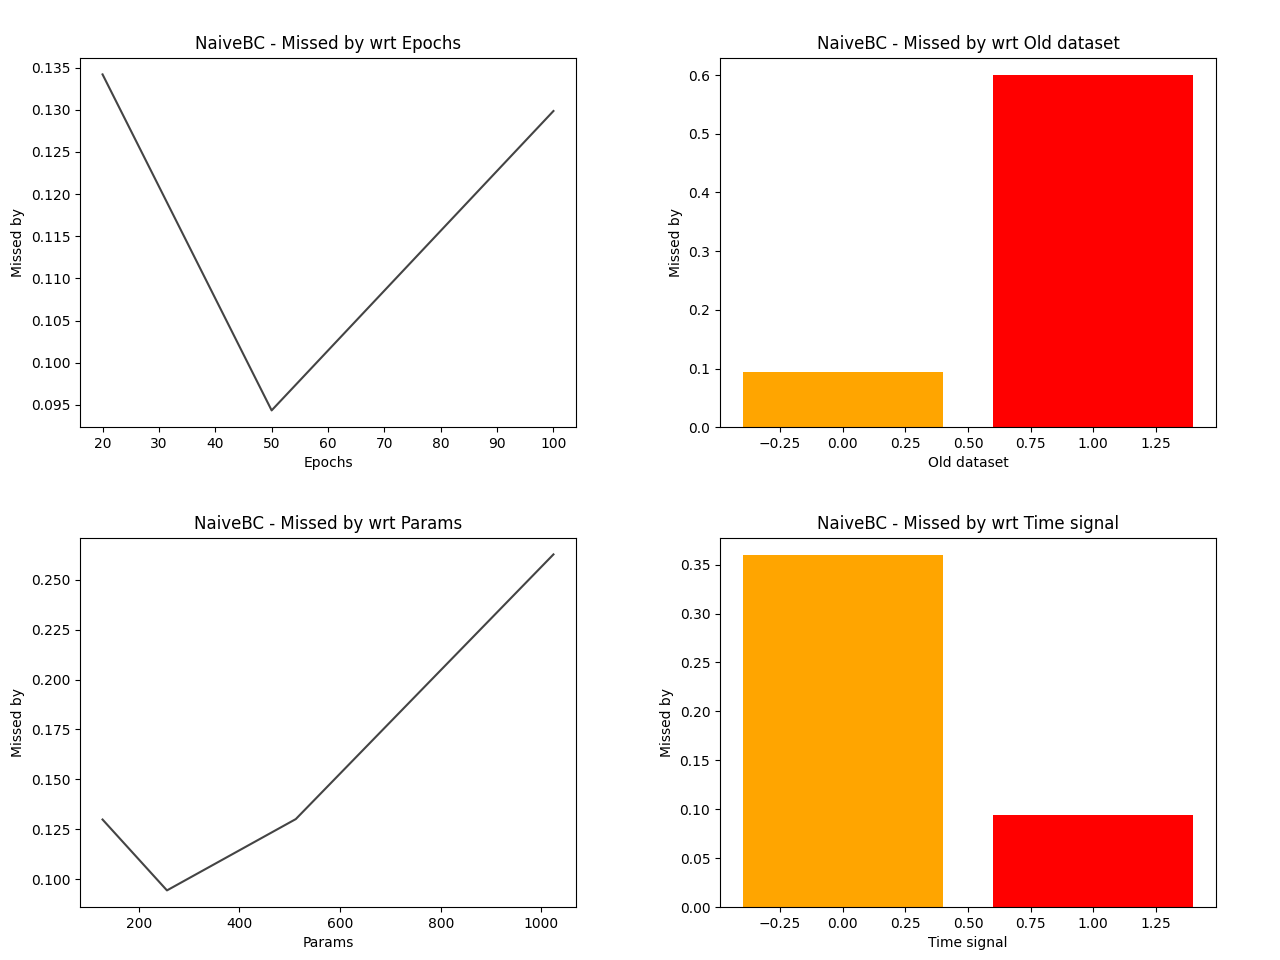
\includegraphics[width=16cm,page=1]{../img/naivebc_missed.png}
    \caption{Klasiskā neironu tīkla ģenerēto trajektoriju simulēto metienu nobīdes atkarībā no: apmācības epohu skaita; jaunās/vecās datu kopas; parametru skaita; laika signāla neesamības/esamības.}
\end{figure}

12. attēlā savukārt salīdzināti metiena novērtējumi. Redzams, ka ātruma vektora nobīdes vērtējumos rekurentais tīkls pārspēj klasisko. Pozīcijas kļūda abos gadījumos ir neliela, taču labāko rezultātu šajā gadījumā ir sasniedzis klasisks modelis. Taču pārstei-dzošā kārtā, arī labāko rezultātu simulētā metiena nobīdē sasniedz viens no parastajiem modeļiem, kaut gan atšķirība ir ļoti neliela un precizitāte abiem modeļiem ir ~0,1m diapazonā. Kā apspriests zemāk pie divu izmantoto demonstrāciju kopu salīdzinājuma, tas visticamāk skaidrojams ar nelielo validācijas kopu ``mazo metienu'' korpusā -- novedot pie lielākas dispersijas šajā kvalitātes mērā. Attēloti arī daži rezultāti, kas gūti, sākot GAN modeļa attīstību. Kā redzams, sasniegta modeļa konverģence -- vērtējamie kritēriji manāmi uzlabojas, pieaugot treniņa epohu skaitam. Taču vēl nav sasniegta konkurētspējīga veiktspēja, tāpēc šī darba ietvaros sīkāk rezultāti pētīti netiks. 

\begin{figure}[t!]
    \centering
    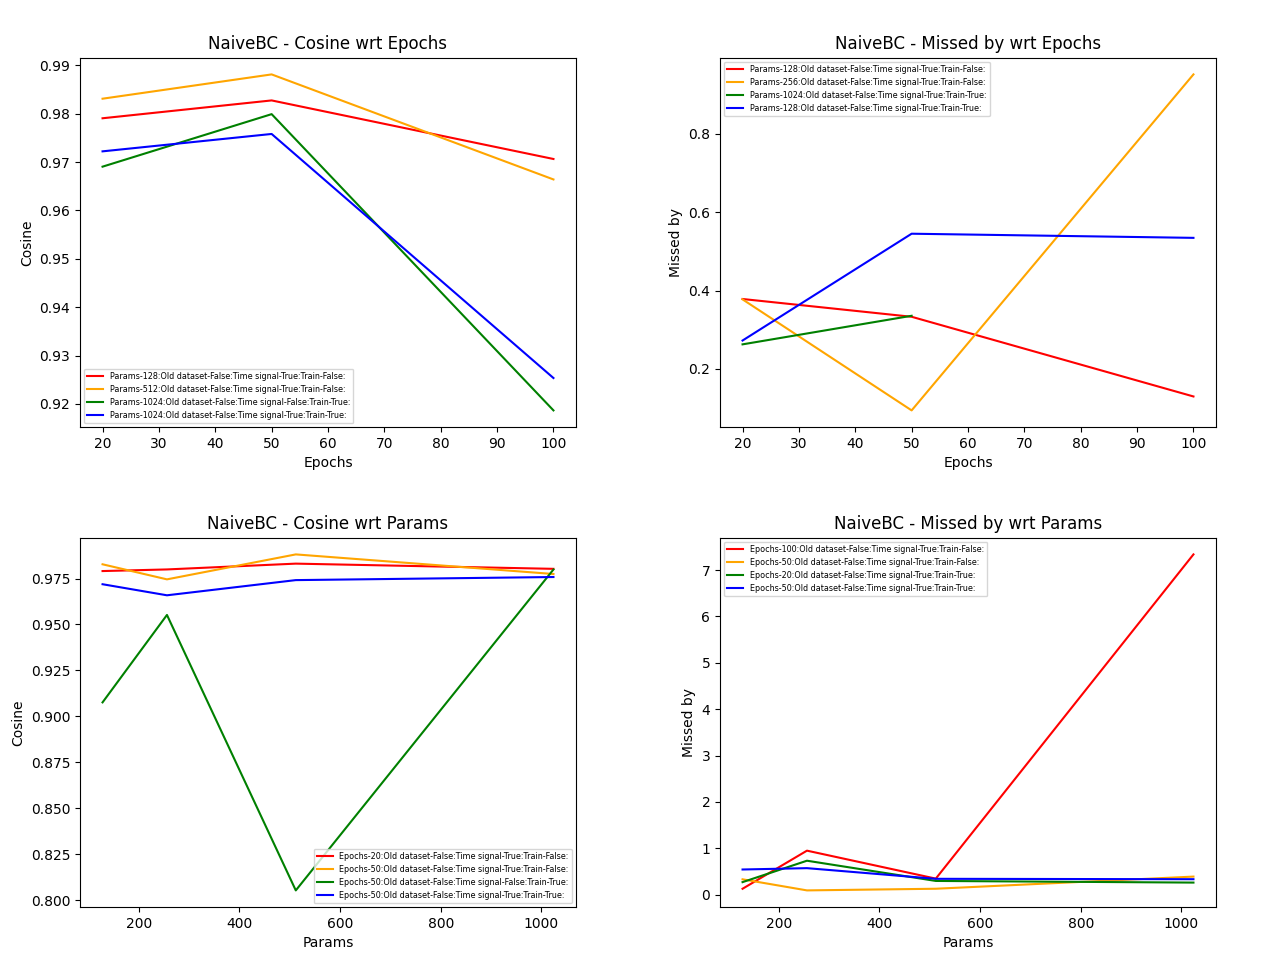
\includegraphics[width=16cm,page=1]{../img/naivebc-independent-params-epoch.png}
    \caption{Atsevišķu klasisko modeļu novērtējumi, mainot tikai vienu hiperparametru. Augšējā rindā kosinusu līdzība un metiena kļūda atkarībā no epohas, apakšējā -- no parametru skaita.}
\end{figure}

\subsection{Klasiskie neironu tīkli}


13. attēlā redzamas galvenās atziņas, kas gūtas strādājot ar parasto neironu tīklu -- labākie rezultāti pie katras attēlotā hiperparametra vērtības. Gan pret epohu skaitu, gan modeļa izmēriem novērotās sakarības liecina, ka problēmas dinamikas modelēšanai varētu būt samērā nedaudzas brīvības pakāpes. Līdz ar to neliels modelis un ne pārāk ilga apmācība ir pietiekami -- pēc tam veiktspēja atkal samazinās, visticamāk pārpielāgošanās rezultātā. Labākie rezultāti gūti pie 256 perceptroniem katrā slēptajā slānī un 50 treniņa epohām. 


14. attēlā redzamas izmaiņas novērtējumos atkarībā tikai no viena mainīgā lieluma. Var secināt, ka klasiskā modeļa līdzība ar demonstrāciju sadalījumu sāk kristies, pieaugot epohu skaitam, un abi labajā pusē redzami grafiki parāda, ka iespējams novērot pārpielāgošanos uz validācijas kopas. Interesanti, ka kosinusu līdzībai pie dažādiem para-metru skaitiem var būt ievērojama dispersija pat bez skaidri redzama kāpuma vai krituma.

\begin{figure}[t!]
    \centering
    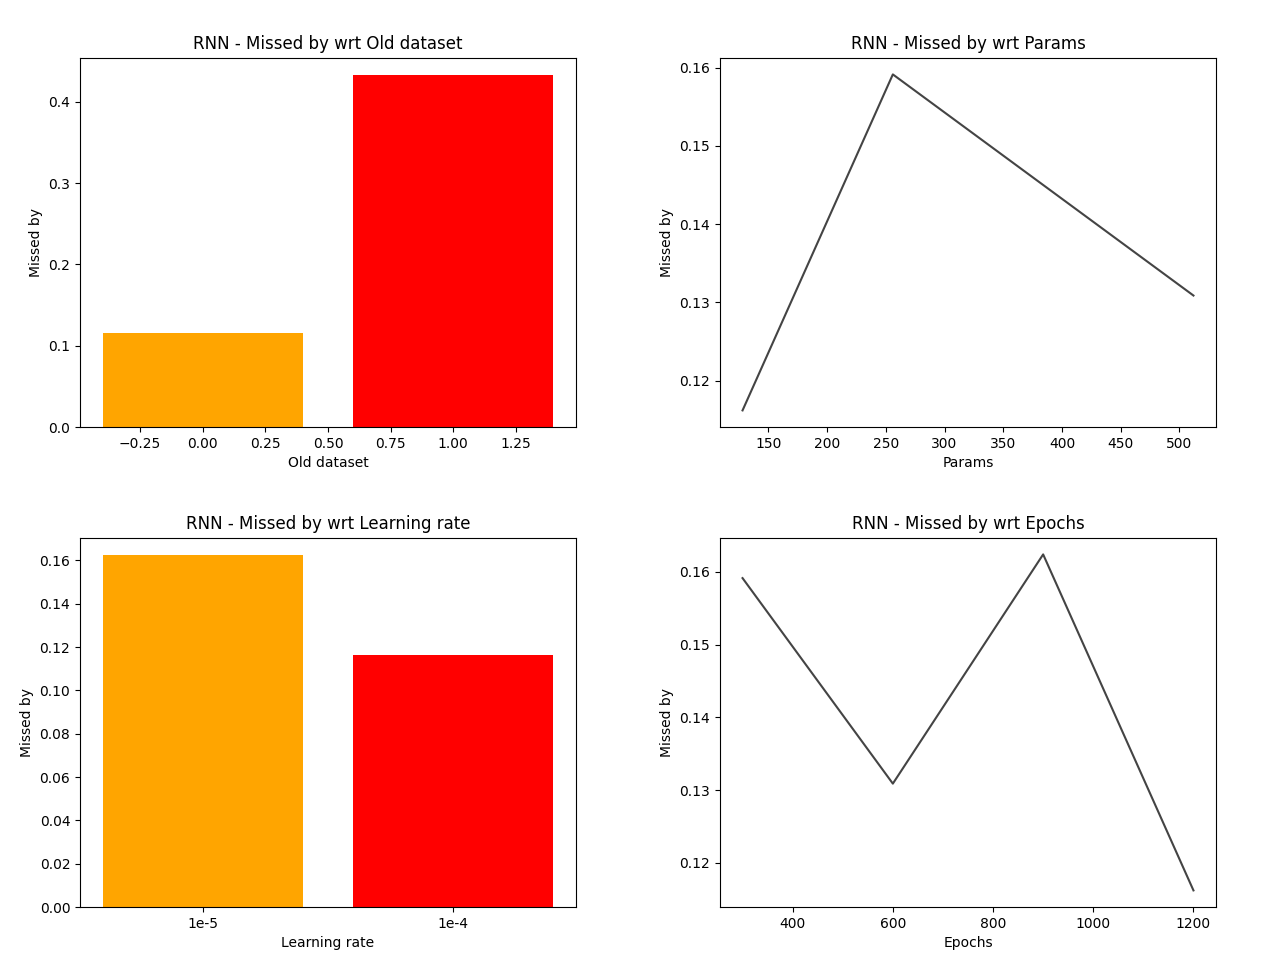
\includegraphics[width=16cm,page=1]{../img/rnn_missed.png}
    \caption{Rekurentā neironu tīkla ģenerēto trajektoriju simulēto metienu nobīdes atkarībā no: datu kopas; parametru skaita; apmācības ātruma; epohu skaita.}
\end{figure}

Pirmās datu korpusa versijas tika sagatavotas bez atsevišķa laika signāla -- balstoties uz pieņēmumu, ka orientācijas izmaiņa varētu būt pietiekama, lai dotu stratēģijai kontekstu par to, kurā metiena fāzē tā šobrīd atrodas. Savā ziņā pieņēmums apstiprinājās -- modelis konverģē, un arī kaut kas līdzīgs metienam tiek noģenerēts. Taču, kā redzams rezultātos, pievienojot atsevišķu laika signālu vektoram rezultāti tiek radikāli uzlaboti.



Visbeidzot, lielākā daļa demonstrāciju tikušas ierakstītas vairākās stadijās vēl mē-nešus pirms autoregresijas rezultātus mēģināts atkārtot ar fizisku robotu. Izrādās, ka tās neatbilst robota izmēriem -- veiktie vēzieni ir pārāk lieli, un mēģinājumi proporcionāli koriģēt tos noved pie nesakritības starp efektora pozīciju un orientāciju (tiek mēģināts lielas rotācijas apvienot ar nelieliem pārvietojumiem, kas noved pie bremzēšanas reālā robotā). Tāpēc neilgi pirms darba noslēguma iegūta jauna demonstrāciju kopa, kas gan ir mazāka par veco. Protams, arī validācijas kopa ir attiecīgi mazāka.  Tajā ir līdzīga mērķa koordinātu dispersija un, varbūt svarīgāk, tās ir tuvāk metiena sākumpunktam. Augstākās simulēto metienu precizitātes sasniegtas tieši uz šīs kopas. Mazākas absolūtās vērtības kombinētas ar relatīvi lielāku dispersiju liek domāt, ka varētu būt ievērojams nejaušības faktors labāko metienu mērā. Turpmākiem pētījumiem nepieciešams strādāt ar lielāku validācijas kopu. Tomēr jāpiebilst, ka vecajā datu kopā sasniegtās precizitātes patiešām varētu būt zemākas, jo tajā ir daudz lielāka \textit{sākuma orientāciju} dispersija -- rezultātā modelis paredz agresīvākas rotācijas, bet validācijas trajektorijas ievāktas ar neitrālu sākuma stāvokli.

\subsection{Rekurentie neironu tīkli}

\begin{figure}[t!]
    \centering
    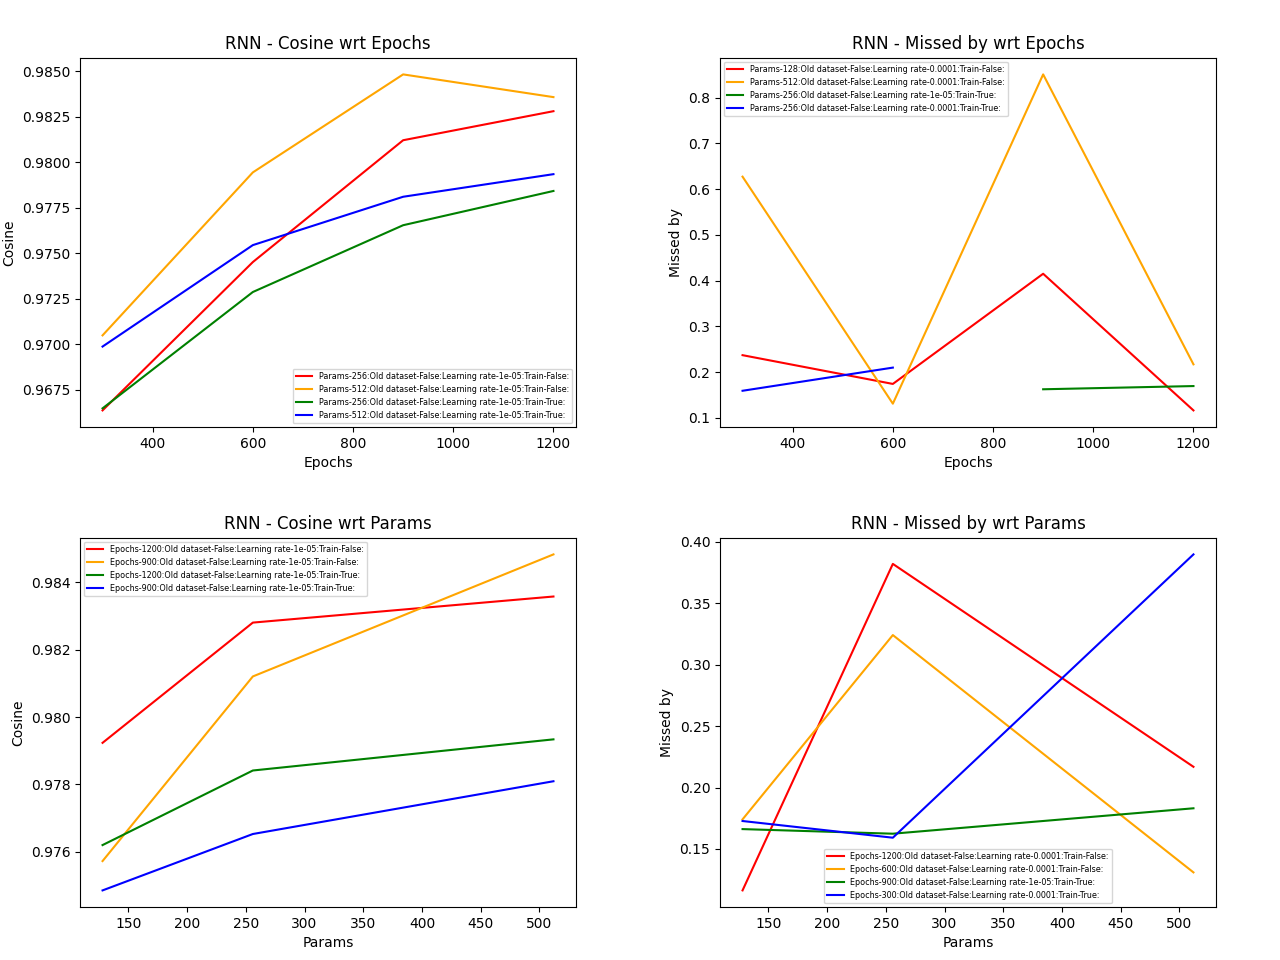
\includegraphics[width=16cm,page=1]{../img/rnn-independent-params-epoch.png}
    \caption{Atsevišķu rekurento modeļu novērtējumi, mainot tikai vienu hiperparametru. Augšējā rindā kosinusu un metiena kļūda atkarībā no epohas, apakšējā -- no parametru skaita.}
\end{figure}

15. attēlā salīdzināta rekurentā tīkla simulēto metienu precizitāte pie dažādiem hiperparametriem. Pirmkārt, redzams, ka ne pēc epohām, ne modeļa izmēriem skaidras sakarības nav novērojamas -- vērtībām ir ļoti neliela dispersija. Tas rada zināmas cerības, ka vēl nav atrastas optimālas hiperparametru kombinācijas, un iespējami tālāki uzlabojumi. Svarīgi arī pamanīt, ka pie vecās datu kopas -- kas ir lielāka un ar daudz lielākām efektora orientācijas izmaiņām -- rekurentais modelis sasniedz ievērojami labākus rezul-tātus, nekā klasiskais. Tomēr pie nelielās jaunā datu korpusa validācijas kopas sasniegtā precizitāte ir mazliet zemāka.


16. attēlā redzami rekurentā tīkla novērtējumu izmaiņas, noturot fiksētus pārējos hiperaparametrus. Redzams, ka epohu skaits lielākiem modeļiem (ar 256, 512 perceptroniem katrā slēptajā slānī) noved pie augstākiem kopējās līdzības novērtējumiem (šajā gadījumā, kosinusu), taču sakarība nav tik viennozīmīga, apskatot metiena kļūdu. Tāpat kā iepriekš, katrā grafikā attēloti četri modeļi ar absolūti labākajām sasniegtajām vērtībām -- divi pret treniņa kopu un divi pret testa. Redzams, ka, salīdzinot ar nelielās validācijas kopas trajektorijām, abi modeļi visos gadījumos ir veiksmīgi padevuši atlaišanas signālu, taču pie lielākās apmācības kopas abiem modeļiem tas notiek tikai konkrētā epohu diapazonā. Turklāt izteikta kļūst apmācības ātruma ietekme uz rezultātiem. 256-neironu modelis ar apmācības ātrumu $\lambda = 10^{-5}$ ir lietojams pie 900 vai 1200 epohām, bet ar ātrumu $\lambda = 10^{-4}$ -- pie 300 vai 600. 

Apakšējā rindā kā mainīgais hiperparametrs izmantots perceptronu skaits modelī. kosinusu līdzības grafiks parāda, ka faktiski modeļa spēja apgūt datu kopu vai to ģene-rējošo sadalījumu vēl joprojām pieaug (kaut gan lēni), palielinot parametru skaitu pie dažādām pārējo hiperparametru kombinācijām. Savukārt metienu kļūda pret validācijas kopu liecina, ka pie 300 epohām pat ar augstāku apmācības ātrumu lielākais 512-neironu modelis vēl nav pietiekami labi apguvis sadalījumu. Pie 900 epohām iegūtie rezultāti uz validācijas kopas ir diezgan stabili, kas gan iespējams skaidrojams ar šīs kopas nelielo izmēru. Interesanti, ka pret apmācības kopu un lielāka epohu skaita gan 128, gan 512 peceptronu varianti pārspēj vidējo 256-neironu modeli -- iespējams, liecinot par t.s. divkāršā krituma jeb \textit{``double descent''} fenomenu \cite{nakkiran2021deep}.


%
%
%
%
%
%
%
%
%
%
% CHAPTER 8
% CHAPTER 8
% CHAPTER 8
% CHAPTER 8
% CHAPTER 8
% CHAPTER 8
% CHAPTER 8
% CHAPTER 8
% CHAPTER 8
% CHAPTER 8
% CHAPTER 8
% CHAPTER 8
% CHAPTER 8
%
%
%
%
%
%
%
%
%


\newpage
\phantomsection
\section*{Secinājumi} % * nepieliks numuru pie nosaukuma
\addcontentsline{toc}{section}{Secinājumi}

Veicot literatūras analīzi, identificēti Robotikas un mašīnuztveres laboratorijas mēr-ķiem un iespējām atbilstošākie potenciālie risinājumi motivējošajam uzdevumam -- MDP formālismam atbilstoša uzvedības klonēšana ar klasisku neironu tīklu kā stratēģiju un no laikrindu prognozēšanas metodēm aizgūta rekurentā tīkla pielietojums. Attīstītā automatizētā datu ieguves un priekšapstrādes sistēma ir adekvāta, lai ātri un sistemātiski sagatavotu demonstrāciju trajektoriju kopas no ierakstiem ar minimālu cilvēka iesaisti. Ar iegūtajiem datiem apmācītie klasiskie un rekurentie modeļi kvalitatīvi labi aproksimē metienus, un pārbaudot rezultātu uz fiziska robota var pārliecināties, ka pat ar neprecīzu laika parametrizāciju jau iespējams izpildīt metiena kustību.

Salīdzinot apmācītos modeļus, redzams, ka daudzos statistiskos novērtējumos sarež-ģītākais rekurentais tīkls pārspēj klasisko neironu tīklu, taču pagaidām grūti spriest, vai sniegtie uzlabojumi ir pietiekami, lai atsvērtu modeļa lielāko sarežģītību gan no izpildījuma, gan asimptotiskās laika sarežģītības puses. Katrā ziņā ļoti aptuvenajā metiena trāpīguma novērtējumā pagaidām labāko rezultātu sasniedz klasiskais neironu tīkls, taču atšķirība ir neliela un tās nozīmīgums ir strīdīgs, jo rezultāts iegūts uz ļoti nelielas validācijas kopas.

Ņemot vērā augstāk minēto pieredzi un atziņas no teorētiskās literatūras, iezīmējas skaidri virzieni tālākai pētnieciskai un inženiertehniskai darbībai:

\begin{enumerate}
    \item nepieciešams izstrādāt programmnodrošinājumu precīzi laikā parametrizētu telpisku trajektoriju izpildei ar robotu ROS vidē. Šī darba zinātniskā prioritāte nav augsta, jo komerciāli pielietojamā industriālo robotu vidē šāda tipa funkcionalitāte tiek piedāvāta (piemēram, lineāras kustības instrukcijās ar telpiska ātruma argumentu) \cite{abb_rapid}. Taču šāds rīks būtu nepieciešams tālākai eksperimentālai darbībai, piemēram, salīdzinot dažādu modeļu faktiski sasniegto precizitāti;
    \item nepieciešams ievākt lielākas datu kopas, kas atbilst robota kinemātikas ierobežo-jumiem, it sevišķi validācijas mērķiem;
    \item pastāv iespēja, ka ar noteiktiem uzlabojumiem apmācības procesā pilnīgi pietiek tikai ar MDP formālismam atbilstošām stratēģijām. Viens no papildinājumiem varētu būt jau uzsāktā GAN modeļu izveide, kas teorētiskajā literatūrā sasniedz labākos rezultātus;
    \item modeļus varētu apmācīt tā, lai tie paredz nevis nākamo pozīciju un orientāciju, bet gan telpiskos un leņķiskos ātrumus. Tādā veidā būtu triviāli integrēt modeli ar servokontrolleri;
    \item motivējošais uzdevums -- pudeles metiens -- ir tikai viens no daudziem potenciāliem pielietojumiem sistēmai, kas kustību uztveres radītos datus pārvērš apmācītos robota vadības modeļos. Noderīgi būt atrast citus šādus uzdevumus un pārbaudīt, cik sarežģīti ir vispārināt šī darba ietvaros izveidotās iestrādes citām problēmām. It sevišķi jādomā par to, cik liels papildus darbs nepieciešams, lai pielāgotu priekš-apstrādes sistēmu darbam ar citādiem uzdevumiem, kam pastāv citi kritiskie punkti un aprēķināmie papildu parametri.
\end{enumerate}

\newpage
\phantomsection
\addcontentsline{toc}{section}{Atsauces}
\printbibliography[title=Atsauces]


\newpage
\phantomsection
\section*{Dokumentārā lapa}
\thispagestyle{empty}

Maģistra darbs ``Atdarinošās mašīnmācīšanās pielietojums robotikā'' izstrādāts LU Datorikas fakultātē. \bigbreak

Darba teksta galīgā versija izgatavota 23.05.2022. \bigbreak

Ar savu parakstu apliecinu, ka pētījums veikts patstāvīgi, izmantoti tikai tajā norādī-tie informācijas avoti un iesniegtā darba elektroniskā kopija atbilst izdrukai. \bigbreak

Autors: \underline{\hspace{7cm}} (Autora paraksts un datums) \bigbreak

Ar savu parakstu apliecinu, ka esmu lasījis augstāk minēto maģistra darbu un atzīstu
to par p i e m ē r o t u / n e p i e m ē r o t u (nevajadzīgo svītrot) aizstāvēšanai Latvijas Universitātes datorzinātņu maģistrantūrā. \bigbreak

Darba vadītājs: \underline{\hspace{5cm}} (Autora paraksts un datums) \bigbreak

Darbs iesniegts maģistrantūas sekretariātā  \underline{\hspace{3cm}} (Iesniegšanas datums) \bigbreak

Ar šo es apliecinu, ka darba elektroniskā versija ir augšupielādēta LU informatīvajā sistēmā.

Studiju metodiķe: \underline{\hspace{5cm}} (Metodiķes paraksts) \bigbreak

Recenzents: prof. Dr. dat. Guntis Bārzdiņš \bigbreak

Darbs aizstāvēts maģistra gala pārbaudījuma komisijas sēdē \bigbreak

\underline{\hspace{5cm}} prot. Nr. \underline{\hspace{3cm}} \bigbreak

Komisijas sekretārs: \underline{\hspace{5cm}} (Sekretāra paraksts)



\end{document}